%!TEX TS-program = pdflatex
% dissertation.tex -- main dissertation file
%
% Wisconsin dissertation template
% Copyright (c) 2008-2009 William C. Benton.  All rights reserved.
%
% This program can redistributed and/or modified under the terms
% of the LaTeX Project Public License Distributed from CTAN
% archives in directory macros/latex/base/lppl.txt; either
% version 1 of the License, or (at your option) any later version.
%
% This program includes other software that is licensed under the
% terms of the LPPL and the Perl Artistic License; see README for details.
%
% You, the user, still hold the copyright to any document you produce
% with this software (like your dissertation).
%

%%% You'll want ``oneside'' for the deposit version, but probably not for any versions that don't need to meet the UW requirements
\documentclass[12pt,oneside,letterpaper]{memoir}
\usepackage{wrapfig}
\usepackage[percent]{overpic}
\usepackage{color}
\usepackage{caption}
\usepackage{subcaption}
\usepackage{amsthm}
\usepackage{amsmath}
\usepackage[chapter]{algorithm}
\usepackage{tikz}
\usepackage{changebar}
\usepackage{adjustbox}
\usepackage{algorithmic}
\usepackage{framed}
\usepackage{xcolor}
\definecolor{shadecolor}{gray}{0.9}
\usetikzlibrary{decorations.pathreplacing}
\theoremstyle{plain}
\newtheorem{thmN}{Theorem}[chapter] % reset theorem numbering for each chapter
\newtheorem{lem}[thmN]{Lemma}

\theoremstyle{definition}
\newtheorem{defn}[thmN]{Definition} % definition numbers are dependent on theorem numbers
\newtheorem{exmp}[thmN]{Example} % same for example numbers

% customising the new block
\newcommand{\varA}[1]{{\operatorname{#1}}}
\newcommand{\varB}[1]{{\operatorname{\mathit{#1}}}}
\newcommand{\tikzmark}[1]{\tikz[overlay,remember picture,baseline=(#1.base)]
  \node (#1) {\strut};}
  
\newcommand{\removed}[1]{} % non-markup version

% preamble.tex -- packages to include
%
% Wisconsin dissertation template
% Copyright (c) 2008 William C. Benton.  All rights reserved.
%
% This program can redistributed and/or modified under the terms
% of the LaTeX Project Public License Distributed from CTAN
% archives in directory macros/latex/base/lppl.txt; either
% version 1 of the License, or (at your option) any later version.
%
% This program includes other software that is licensed under the
% terms of the LPPL and the Perl Artistic License; see README for details.
%
% You, the user, still hold the copyright to any document you produce
% with this software (like your dissertation).

%% You should use natbib
\IfFileExists{natbib.sty}{%
\usepackage{natbib}%
}{}

%% You probably need appendix, if you want appendices
\IfFileExists{appendix.sty}{%
\usepackage{appendix}%
}{}

%% the spacing in memoir is weird, you'll need to use this
\DisemulatePackage{setspace}
\usepackage[onehalfspacing]{setspace}

%% List setup; the ``hanglist`` environment will allow you to have
%% nicely-typeset enumerated lists (i.e. with the numbers hanging in
%% the margins).  You need at least version 2.1 of enumitem.sty.  If
%% you don't have enumitem installed at all, hanglist will just be an
%% alias for enumerate.
\IfFileExists{enumitem.sty}{%
\usepackage[loadonly]{enumitem}[2007/06/30]%
\newlist{hanglist}{enumerate}{1}% 
\setlist[hanglist]{label=\arabic*.}%
\setlist[hanglist,1]{leftmargin=0pt}%
}{%
\newenvironment{hanglist}{\begin{enumerate}}{\end{enumerate}}%
}

%% Comment out any of these that you don't want
\usepackage{amssymb}
\usepackage{amsmath}
\usepackage{amsthm}
%\usepackage{theorem}
\usepackage{hyperref}

\IfFileExists{mathpartir.sty}{%
\usepackage{mathpartir}%
}{}

%%%%% LISTINGS package and setup
\IfFileExists{listings.sty}{%
\usepackage{listings}%
}{}



%% Get rid of ugly borders around PDF hyperlinks (e.g. for cross-references, bib entries, or URLs)
\hypersetup{pdfborder = 0 0 0}

%% You want microtype.
\IfFileExists{microtype.sty}{%
\usepackage[protrusion=true,expansion=true]{microtype}%
}{}

%\pagestyle{thesisdraft}

% Surround parts of graphics with box
\usepackage{boxedminipage}

%% booktabs (thx to Nate Rosenblum for bringing this beautiful package
%% to my attention)
\IfFileExists{booktabs.sty}{%
\usepackage{booktabs}%
}{}

% This is now the recommended way for checking for PDFLaTeX:
\usepackage{ifpdf}

%% Avoid ugly "Type 3" fonts
\usepackage{lmodern}
\usepackage[LY1]{fontenc}

%% Substitute your favorite serif and sans fonts here....
\IfFileExists{tgpagella.sty}{%
% TeX Gyre pagella, like Palatino
\usepackage{tgpagella}%
}{}

\usepackage[LY1]{eulervm}

\ifpdf
\usepackage[pdftex]{graphicx}
\else
\usepackage{graphicx}
\fi

\usepackage{makeidx}
\makeindex

{\theoremstyle{plain}
\newtheorem{thm}{Theorem}[chapter]
\newtheorem{cor}[thm]{Corollary}
\newtheorem{define}[thm]{Definition}
\newtheorem{exmpl}[thm]{Example}
}
{\theoremstyle{remark}
\newtheorem{rmk}[thm]{Remark}
}

\newtheoremstyle{customsty1}
{3pt}%
{3pt}%
{}% --- body font
{}% --- indent amount
{\bfseries}% --- Theorem head font
{:}% --- Punctuation after head
{.5em}% --- space after head
{}% --- theorem head spec (can be left empty, meaning 'normal')

% Define 'newtheorems' that use ``customsty1''
{\theoremstyle{customsty1} 
}


%%% NB: the ``deposit'' chapter- and page- styles should conform to UW
%%% requirements.  If you are producing a pretty version of your
%%% dissertation for web use later, you will certainly want to make
%%% your own chapter and page styles.

\makechapterstyle{deposit}{%
  \renewcommand{\chapterheadstart}{}
  \renewcommand{\printchaptername}{}
  \renewcommand{\chapternamenum}{}
  \renewcommand{\printchapternum}{\parbox{2em}{\MakeLowercase{\Large\scshape\thechapter{}}} }
  \renewcommand{\afterchapternum}{}
  \renewcommand{\printchaptertitle}[1]{%
  \raggedright\Large\scshape\MakeLowercase{##1}}
  \renewcommand{\afterchaptertitle}{%
  \vskip\onelineskip \hrule\vskip\onelineskip}
}

\makepagestyle{deposit}
 
\makeatletter
 
\renewcommand{\chaptermark}[1]{\markboth{#1}{}}
\renewcommand{\sectionmark}[1]{\markboth{#1}{}}
 
\makeevenfoot{deposit}{}{}{}
\makeoddfoot{deposit}{}{}{}
\makeevenhead{deposit}{\thepage}{}{}
\makeoddhead{deposit}{}{}{\thepage}
\makeatother

%%% set up page numbering for chapter pages to satisfy UW requirements
%%% NB: You will want to delete until the ``SNIP'' mark if you are
%%% making a ``nice'' copy
\copypagestyle{chapter}{plain}
\makeoddfoot{chapter}{}{}{}
\makeevenhead{chapter}{\thepage}{}{}
\makeoddhead{chapter}{}{}{\thepage}
%%% SNIP

%%% bib nonsense
\makeatletter
\newenvironment{wb-bib}[1]{%
  \chapter*{references}
\ifnobibintoc\else 
\phantomsection 
\addcontentsline{toc}{chapter}{References} 
\fi 
\prebibhook
  \begin{bibitemlist}{#1}}{\end{bibitemlist}\postbibhook}

\AtBeginDocument{%
  \@ifpackageloaded{natbib}{% natbib is loaded
    \addtodef{\endthebibliography}{}{\vskip-\lastskip\postbibhook}
    \@ifpackagewith{natbib}{sectionbib}{% with sectionbib option
      \renewcommand{\bibsection}{\@memb@bsec}}%
      {\renewcommand{\bibsection}{\@memb@bchap}}}%
  {}
  \@ifpackagewith{chapterbib}{sectionbib}{%
    \renewcommand{\sectionbib}[2]{}
    \renewcommand{\bibsection}{\@memb@bsec}}{}
}
\makeatother


% defs.tex -- wbepi environment for chapter epigraphs and other useful defs.
%
% Wisconsin dissertation template
% Copyright (c) 2008 William C. Benton.  All rights reserved.
%
% This program can redistributed and/or modified under the terms
% of the LaTeX Project Public License Distributed from CTAN
% archives in directory macros/latex/base/lppl.txt; either
% version 1 of the License, or (at your option) any later version.
%
% This program includes other software that is licensed under the
% terms of the LPPL and the Perl Artistic License; see README for details.
%
% You, the user, still hold the copyright to any document you produce
% with this software (like your dissertation).


%% put lstnewenvironment declarations here, if you're using listings

%% end lstnewenvironment declarations

%% I put convenience definitions that will go in several chapters here

%%%%% begin convenience definitions

\makeatletter
\newcommand{\wb@episource}{}
\newenvironment{wbepi}[1]{\begin{quote}\renewcommand{\wb@episource}{#1}\itshape}{\par\upshape \raggedleft --- \textsc{\wb@episource}\\ \end{quote}}
\makeatother

%%%%% SVN
\IfFileExists{svn-multi.sty}{%
\usepackage{svn-multi}%
%%% Uncomment the second one and comment out the first one if you want
%%% to include subversion revision information in each file.
\newcommand{\vcinfo}{}%
%\newcommand{\vcinfo}{\begin{centering}\fbox{\fbox{\parbox{5in}{Author: \svnauthor\\Revision: \svnfilerev\\Last changed on: \svnfiledate\\URL: \svnkw{HeadURL}}}}\\[1em]\end{centering}}%
}{%
\newcommand{\svnidlong}[4]{}%
\newcommand{\svnfilerev}{}%
\newcommand{\svnauthor}{}%
\newcommand{\svnfiledate}{}%
\newcommand{\svnkw}{}%
\newcommand{\vcinfo}{}%
}

%%%%% end convenience definitions

% thesisdefs.tex

% This is mostly adapted from withesis.cls.  The original copyright
% notice for withesis.cls follows, preceded by two percent signs (%%):

%% withesis.cls
%% LaTeX Style file for the University of Wisconsin-Madison Thesis Format
%% Adapted from the Purdue University Thesis Format
%% Originally by Dave Kraynie
%% Edits by Darrell McCauley
%% Adapted to UW-Madison format by Eric Benedict  (Noted with <EB>)
%% Updated to LaTeX2e by Eric Benedict 24 July 00
%% 
%%=============================================================================
%% Licensed under the Perl Artistic License.
%% see: http://www.ctan.org/tex-archive/help/Catalogue/licenses.artistic.html
%% for more info...
%%=============================================================================

% withesis.cls is available from CTAN.  The modifications to this file
% are also licensed under the Perl Artistic License.

% --wb, 2008

\makeatletter

\newcounter {tocpage}
\newcounter {lofpage}
\newcounter {lotpage}
\newcounter {listofheading}

\newcommand\@thesistitlemedskip{0.2in}
\newcommand\@thesistitlebigskip{0.6in}
\newcommand{\degree}[1]{\gdef\@degree{#1}}
\newcommand{\project}{\gdef\@doctype{A masters project report}}
\newcommand{\prelim}{\gdef\@doctype{A preliminary report}}
\newcommand{\thesis}{\gdef\@doctype{A thesis}}
\newcommand{\dissertation}{\gdef\@doctype{A dissertation}}
\newcommand{\department}[1]{\gdef\@department{(#1)}}

\newenvironment{titlepage}
 {\@restonecolfalse\if@twocolumn\@restonecoltrue\onecolumn
  \else \newpage \fi \thispagestyle{empty}
% \c@page\z@ -- deleted: count title page in thesis
}{\if@restonecol\twocolumn \else \newpage \fi}

\gdef\@degree{Doctor of Philosophy}    %Default is PhD
\gdef\@doctype{A dissertation}         %Default is dissertation

\gdef\@department{(Electrical Engineering)} % Default is Electical Engineering
\gdef\@defensedate{01/01/2100}% Default is a long time from now.
\gdef\@committee{
  Jane Doeverything, Professor, Electrical Engineering\\
  John Dosomethings, Associate Professor, Electrical Engineering\\
  }

\renewcommand{\maketitle}{%
  \begin{titlepage}
%-----------------------------------------------------------------------------
% -- The thesis office doesn't like thanks on title page.  Put it in
% -- the acknowledgments.  This is here so you don't have to change
% -- your titlepage when converting from report style. -> from Purdue, but I
%        left it here since it seems compatible with UW-Madison, Eric
%-----------------------------------------------------------------------------
    \def\thanks##1{\typeout{Warning: `thanks' deleted from thesis titlepage.}}
    \let\footnotesize\small \let\footnoterule\relax \setcounter{page}{1}
    \begin{center}
      {\textbf{\expandafter\expandafter{\@title}}} \\[\@thesistitlebigskip]
       by \\[\@thesistitlemedskip]
      \@author \\[\@thesistitlebigskip]
      \@doctype\ submitted in partial fulfillment of \\
      the requirements for the degree of\\[\@thesistitlebigskip]
      \@degree \\[\@thesistitlemedskip]
      \@department \\[\@thesistitlebigskip]
      at the \\[\@thesistitlemedskip]
      UNIVERSITY OF WISCONSIN--MADISON\\[\@thesistitlemedskip]
      \@date
    \end{center}
    \hspace*{-0.7in}Date of final oral examination: \@defensedate \\[\@thesistitlemedskip]
    \hspace*{-0.7in}The dissertation is approved by the following members of the 
    Final Oral Committee:\\
    \@committee
  \end{titlepage}
  \setcounter{footnote}{0}
  \setcounter{page}{1} %title page is NOT counted
  \let\thanks\relax
  \let\maketitle\relax \let\degree\relax \let\project\relax \let\prelim\relax
  \let\department\relax
  \gdef\@thanks{}\gdef\@degree{}\gdef\@doctype{}
  \gdef\@department{}
  %\gdef\@author{}\gdef\@title{}
}


%=============================================================================
% ABSTRACT
%=============================================================================
% The abstract should begin with two single-spaced lines describing
% the author and title in a standard format.  After these lines comes
% the standard abstract.
%=============================================================================
\def\abstract{
  \chapter*{Abstract}
  \addcontentsline{toc}{chapter}{Abstract}
  \relax\markboth{Abstract}{Abstract}}
\def\endabstract{\par\newpage}


%=============================================================================
% UMI ABSTRACT
%=============================================================================
% The UMI abstract should begin with the author and title in a standard format.
% After the author comes the advisor and university. After these lines comes
% a bunch of double spaced text to make up the standard abstract.
% After the abstract, the advisor's approval signature follows.
% This page is not numbered and is delivered seperately to the thesis office.
%=============================================================================

\def\advisortitle#1{\gdef\@advisortitle{#1}}
\def\advisorname#1{\gdef\@advisorname{#1}}
\gdef\@advisortitle{Professor}
\gdef\@advisorname{Cheer E.\ Place}

\def\umiabstract{
             \thispagestyle{empty}
                  \addtocounter{page}{-1}
                \begin{center}
                  {\textbf{\expandafter\uppercase\expandafter{\@title}}}\\
                  \vspace{12pt}
                  \@author \\
                  \vspace{12pt}
                  Under the supervision of \@advisortitle\ \@advisorname\\
                  At the University of Wisconsin-Madison
                \end{center}
}

\def\endumiabstract{\vfill \hfill\@advisorname\par\newpage}


%============================================================================
% VERBATIMFILE
%============================================================================
% \verbatimfile{<filename>}    for verbatim inclusion of a file
% - Note that the precise layout of line breaks in this file is important!
% - added the \singlespace - EB
%============================================================================
\def\verbatimfile#1{\begingroup \singlespace
                    \@verbatim \frenchspacing \@vobeyspaces
                    \input#1 \endgroup
}


%=============================================================================
% SEPARATOR Pages
%   Creates a blank page with a text centered horizontally and vertically.
%   The page is neither counted nor numbered.
%   These pages are required in the thesis format before sections such
%   as appendices, vita, bibliography, etc.
%=============================================================================
\def\separatorpage#1{
  \newpage
  \thispagestyle{empty}
  \addtocounter{page}{-1}
  \null
  \vfil\vfil
  \begin{center}
    {\textbf{#1}}
  \end{center}
  \vfil\vfil
  \newpage}


%=============================================================================
% COPYRIGHTPAGE
%=============================================================================
% The copyright must do the following:
% - start a new page with no number
% - place the copyright text centered at the bottom.
%=============================================================================
\def\copyrightpage{
  \newpage
  \thispagestyle{empty}    % No page number
  \addtocounter{page}{-1}
  \chapter*{}            % Required for \vfill to work
  \begin{center}
   \vfill
   \copyright\ Copyright by \@author\ \@date\\
   All Rights Reserved
  \end{center}}


%=============================================================================
% GLOSSARY
%=============================================================================
% The glossary environment must do the following:
% - produce the table of contents entry for the glossary
% - start a new page with GLOSSARY centered two inches from the top
%=============================================================================
\def\glossary{
  \chapter*{GLOSSARY}
  \addcontentsline{toc}{chapter}{Glossary}}
\def\endglossary{\par\newpage}

%=============================================================================
% NOMENCLATURE
%=============================================================================
% The nomenclature environment must do the following:
% - produce the table of contents entry for the nomenclature section
% - start a new page with NOMENCLATURE centered two inches from the top
%=============================================================================
\def\nomenclature{\separatorpage{DISCARD THIS PAGE}
  \chapter*{Nomenclature}
  \addcontentsline{toc}{chapter}{NOMENCLATURE}}
\def\endnomenclature{\par\newpage}

%=============================================================================
% CONVENTIONS
%=============================================================================
% The conventions environment must do the following:
% - produce the table of contents entry for the nomenclature section
% - start a new page with CONVENTIONS centered two inches from the top
%=============================================================================
\def\conventions{\separatorpage{DISCARD THIS PAGE}
  \chapter*{Conventions}
  \addcontentsline{toc}{chapter}{CONVENTIONS}}
\def\endconventions{\par\newpage}


%=============================================================================
% COLOPHON
%=============================================================================
% The colophon environment must do the following:
% - produce the table of contents entry for the nomenclature section
% - start a new page with COLOPHON centered two inches from the top
%=============================================================================
\def\colophon{\separatorpage{DISCARD THIS PAGE}
  \chapter*{Colophon}
  \addcontentsline{toc}{chapter}{Colophon}}
\def\endcolophon{\par\newpage}

%=============================================================================
% LIST OF SYMBOLS
%=============================================================================
% The list of symbols environment must do the following:
% - produce the table of contents entry for the list of symbols section
% - start a new page with LIST OF SYMBOLS centered two inches from the top
%=============================================================================
\def\listofsymbols{\separatorpage{DISCARD THIS PAGE}
  \eject
  \chapter*{LIST OF SYMBOLS}
  \addcontentsline{toc}{chapter}{LIST OF SYMBOLS}}
\def\endlistofsymbols{\par\newpage}

%=============================================================================
% VITA
%=============================================================================
% The vita environment must do the following:
% - produce a separator page with the word vita centered
% - produce the table of contents entry for the vita
% - start a new page with VITA centered two inches from the top
%=============================================================================
\def\vita{
%  \separatorpage{VITA}         % UW doesn't require this EB
  \chapter*{VITA}
  \addcontentsline{toc}{chapter}{VITA}}
\def\endvita{\par\newpage}

%=============================================================================
% ACKNOWLEDGMENTS
%=============================================================================
% The acknowledgments environment must do the following:
% - start a new page with ACKNOWLEDGMENTS centered two inches from the top
%=============================================================================
\def\acks{
  \chapter*{Acknowledgments}
}
\def\endacks{\par\newpage}

%=============================================================================
% DEDICATION
%=============================================================================
% The dedication environment must do the following:
% - start a new page
% - center the text vertically
% - include the text in a center environment
%=============================================================================
\def\dedication{
  \newpage
  \null\vfil
  \begin{center}}
\def\enddedication{\end{center}\par\vfil\newpage}

%=============================================================================
% DATE
%=============================================================================
%\def\today{\ifcase\month\or
  %January\or February\or March\or April\or May\or June\or
  %July\or August\or September\or October\or November\or December\fi
  %\space\number\day, \number\year}
\newcount\@testday
\def\today{\@testday=\day
  \ifnum\@testday>30 \advance\@testday by -30
  \else\ifnum\@testday>20 \advance\@testday by -20
  \fi\fi
  \number\day\ \
  \ifcase\month\or
    January \or February \or March \or April \or May \or June \or
    July \or August \or September \or October \or November \or December
    \fi\ \number\year
}


%  Single counter for theorems and theorem-like environments:
\newtheorem{theorem}{Theorem}[chapter]
\newtheorem{assertion}[theorem]{Assertion}
\newtheorem{claim}[theorem]{Claim}
\newtheorem{conjecture}[theorem]{Conjecture}
\newtheorem{corollary}[theorem]{Corollary}
\newtheorem{definition}[theorem]{Definition}
\newtheorem{example}[theorem]{Example}
\newtheorem{figger}[theorem]{Figure}
\newtheorem{lemma}[theorem]{Lemma}
\newtheorem{prop}[theorem]{Proposition}
\newtheorem{remark}[theorem]{Remark}

%=============================================================================
% TABLE OF CONTENTS; LIST OF FIGURES; LIST OF TABLES
%=============================================================================
% In report style, \tableofcontents, \listoffigures, etc. are always
% set in single-column style.  @restonecol is used to keep track of
% whether we need to switch back to double column style after the toc.
%
% The only known problem now is that the first page with the new
% layout is too long.  The problem seems to be that the change to
% textheight doesn't take place on the first page.  Even if it's the
% first line in the table of contents macro.  Presumably the same
% problem also occurs in the lof and lot.
%
% I'm taking a shot at fixing the problem by dropping in a throw-away
% page between the change to the height parameters and the start of
% the chapter.  Isn't elegance wonderful?
%
%=============================================================================

% \def\@tableof#1#2#3#4#5{
% { % limit scope of following declarations!!
%   \@restonecolfalse\if@twocolumn\@restonecoltrue\onecolumn\fi
%   \addtolength{\textheight}{-40pt}       % -24-16
%   \addtolength{\majorheadskip}{-40pt}    % -24-16
%   \addtolength{\headheight}{52pt}        %  36+16
%   \addtolength{\headsep}{-12pt}          % -12
%   \separatorpage{DISCARD THIS PAGE}
%   \chapter*{#1}
%   #5
%   \relax\markboth{#1}{#1}
%   \hbox to \hsize{#2 \hfil Page}
%   \singlespace
%   \setcounter{#3}{0}
%   \setcounter{listofheading}{1}  % change from 0 to 1 by mccauley, 14may93
%   \def\@oddhead{\vbox to \headheight{\vspace{4pt}
%     \hbox to \hsize{\hfil\textrm{\thepage}} \vfil
%     \ifnum\value{#3}=1
%       \ifnum\value{listofheading}=2
%         \hbox to \hsize{Appendix\hfil} \vspace{4pt} \fi
%       \ifnum\value{listofheading}=1
%         \stepcounter{listofheading} \fi
%       \hbox to \hsize{#2 \hfil Page}
%     \else
%       \setcounter{#3}{1}
%     \fi}}
%   \def\@evenhead{\vbox to \headheight{\vspace{4pt}
%     \hbox to \hsize{\textrm{\thepage}\hfil} \vfil
%     \ifnum\value{#3}=1
%       \ifnum\value{listofheading}=2
%         \hbox to \hsize{Appendix\hfil} \vspace{4pt} \fi
%       \ifnum\value{listofheading}=1
%         \stepcounter{listofheading} \fi
%       \hbox to \hsize{#2 \hfil Page}
%     \else
%       \setcounter{#3}{1}
%     \fi}}
%   \@starttoc{#4}  \if@restonecol\twocolumn\fi
%   \newpage
% }}
% 
% \def\tableofcontents{\@tableof{TABLE OF CONTENTS}{}{tocpage}{toc}{}}
% 
% \def\listoffigures{
%   \@tableof{LIST OF FIGURES}{Figure}{lofpage}{lof}
%   {\protect\addcontentsline{toc}{chapter}{LIST OF FIGURES}}}
% 
% \def\listoftables{
%   \@tableof{LIST OF TABLES}{Table}{lotpage}{lot}
%   {\protect\addcontentsline{toc}{chapter}{LIST OF TABLES}}}

%=============================================================================
% BIBLIOGRAPHY
%=============================================================================
% The thebibliography environment executes the following commands:
%
%  o start a new 'chapter' with BIBLIOGRAPHY as the heading
%  o produce a separator page for the bibliography
%
%  \def\newblock{\hskip .11em plus .33em minus -.07em} --
%      Defines the `closed' format, where the blocks (major units of
%      information) of an entry run together.
%
%  \sloppy  -- Used because it's rather hard to do line breaks in
%      bibliographies,
%
%  \sfcode`\.=1000\relax --
%      Causes a `.' (period) not to produce an end-of-sentence space.
%=============================================================================
% \altbibtitle
%   The default title for the References chapter is ``LIST OF REFERENCES''
%   Since some people prefer ``BIBLIOGRAPHY'', the command
%   \altbibtitle has been added to change the chapter title.
%   This command does nothing more than change REFERENCES to BIBLIOGRAPHY
%============================================================================
\def\@bibchaptitle{Bibliography}
\def\altbibtitle{\def\@bibchaptitle{Bibliography}}
\def\thebibliography#1{
  %\separatorpage{\@bibchaptitle}
  \global\@bibpresenttrue
  \chapter*{\@bibchaptitle\markboth{\@bibchaptitle}{\@bibchaptitle}}
  \addcontentsline{toc}{chapter}{\@bibchaptitle}
  \vspace{0.375in}    % added to match 4 line requirement
  \interlinepenalty=10000 % added to prevent breaking of bib entries
  \singlespace\list
  {[\arabic{enumi}]}{\settowidth\labelwidth{[#1]}\leftmargin\labelwidth
    \advance\leftmargin\labelsep \usecounter{enumi}}
  \def\newblock{\hskip .11em plus .33em minus -.07em}
  \sloppy
  \sfcode`\.=1000\relax}
\let\endthebibliography=\endlist



\makeatother

\svnidlong{$LastChangedBy$}{$LastChangedRevision$}{$LastChangedDate$}{$HeadURL: http://freevariable.com/dissertation/branches/diss-template/dissertation.tex $} 
\newcommand\numberthis{\addtocounter{equation}{1}\tag{\theequation}}
\graphicspath{ {./images/} }
\clearpage\pagenumbering{roman}  % This makes the page numbers Roman (i, ii, etc)

\title{Designing Efficient Solvers for Large Scale Physics Simulation}
\author{Haixiang Liu}
\department{Computer Sciences}

\date{2018}

\begin{document}

%%% Uncomment the following if your .bib contains references that you will not 
%%% explicitly cite, but that should be in the final bibliography:
% \nocite{*}


\DeclareGraphicsExtensions{.pdf, .jpg, .tif, .png}


\maketitle

%% Add \part declarations if you want, but it's not necessary
%\part{Preliminaries}

\svnidlong{$LastChangedBy$}{$LastChangedRevision$}{$LastChangedDate$}{$HeadURL: http://freevariable.com/dissertation/branches/diss-template/frontmatter/frontmatter.tex $}
\vcinfo{}

%%% SOME OF THIS CODE IS ADAPTED FROM THE VENERABLE withesis.cls

% COPYRIGHT PAGE
%  - To include a copyright page use \copyrightpage
\copyrightpage

% DEDICATION
\begin{dedication}
	\emph{Please insert your dedication here.}
\end{dedication}

%% BEGIN PAGESTYLE

%%% You can pick a pagestyle if you want; see the memoir class
%%% documentation for more info.  The default ``deposit'' option meets
%%% the UW thesis typesetting requirements but is probably
%%% unsatisfactory for making a version of your dissertation that
%%% won't be deposited to the graduate school (e.g. for web or a nice
%%% printed copy)

\chapterstyle{deposit}
\pagestyle{deposit}


% ACKNOWLEDGMENTS
\begin{acks}
\begin{wbepi}{David C.~Makinson (1965)}
It is customary for authors of academic books to include in their prefaces statements such as this: ``I am indebted to ... for their invaluable help; however, any errors which remain are my sole responsibility.'' Occasionally an author will go further. Rather than say that if there are any mistakes then he is responsible for them, he will say that there will inevitably be some mistakes and he is responsible for them....

Although the shouldering of all responsibility is usually a social ritual, the admission that errors exist is not --- it is often a sincere avowal of belief. But this appears to present a living and everyday example of a situation which philosophers have commonly dismissed as absurd; that it is sometimes rational to hold logically incompatible beliefs.
\end{wbepi}

Above is the famous ``preface paradox,'' which illustrates how to use the \texttt{wbepi} environment for epigraphs at the beginning of chapters.  You probably also want to thank the Academy.
\end{acks}

% CONTENTS, TABLES, FIGURES
\renewcommand{\printtoctitle}[1]{\chapter*{#1}}
\renewcommand{\printloftitle}[1]{\chapter*{#1}}
\renewcommand{\printlottitle}[1]{\chapter*{#1}}

\renewcommand{\tocmark}{}
\renewcommand{\lofmark}{}
\renewcommand{\lotmark}{}

\renewcommand{\tocheadstart}{}
\renewcommand{\lofheadstart}{}
\renewcommand{\lotheadstart}{}

\renewcommand{\aftertoctitle}{}
\renewcommand{\afterloftitle}{}
\renewcommand{\afterlottitle}{}

\renewcommand{\cftchapterfont}{\normalfont} 
\renewcommand{\cftsectionfont}{\itshape} 
\renewcommand{\cftchapterpagefont}{\normalfont} 
\renewcommand{\cftchapterpresnum}{\bfseries} 
\renewcommand{\cftchapterleader}{} 
\renewcommand{\cftsectionleader}{} 
\renewcommand{\cftchapterafterpnum}{\cftparfillskip} 
\renewcommand{\cftsectionafterpnum}{\cftparfillskip} 

% \captionnamefont{\small\sffamily} 
% \captiontitlefont{\small\sffamily} 

% \renewcommand{\contentsname}{contents}
% \renewcommand{\listfigurename}{list of figures}
% \renewcommand{\listtablename}{list of tables}

\tableofcontents

\clearpage
\listoftables

\clearpage
\listoffigures

\clearpage
% NOMENCLATURE
% \begin{conventions}
% % \begin{description}
% % \item{\makebox[0.75in][l]{term}
% %        \parbox[t]{5in}{definition\\}}
% % \end{description}
% \input{conventions}
% \end{conventions}

%% The UW graduate school no longer wants a UMI abstract page
%% Should you need one for some reason, uncomment the following
%% lines.  Thanks to Matt Fredrikson for reporting this!

% \advisorname{Gottlob Frege}
% \advisortitle{Professor}
% \begin{umiabstract}
%  Numerical simulation of physical phenomenal has long been of the interests in the area of mechanical engineering, physics, and in recent year computer graphics. The research in the field usually falls into two categories: modeling and solver. Research in modeling intends in finding mathematical equations, sometimes with better accuracy, sometimes are easier to solve, that can be used to describe the physical phenomenal. Research in solvers, on the other hand, is to develop algorithms that are able to solve larger equations faster, for iterative approximate solvers, solve to higher accuracy.  This dissertation focus on designing efficient solvers, centering on a novel data structure namely SPGrid, which provides the flexibility of a sparse and adaptive data structure while retains the performance of a uniform grid. Furthermore, it will present the use of modern Same Instruction Multiple Data(SIMD) hardware and heterogenous platforms that exploits their high computation throughputs to saturate memory utility. Finally, the efficiency of those design principles and practices are demonstrated in the Poisson and Linear elasticity solvers.
% \end{umiabstract}

\begin{abstract}
  Numerical simulation of physical phenomenal has long been of the interests in the area of mechanical engineering, physics, and in recent year computer graphics. The research in the field usually falls into two categories: modeling and solver. Research in modeling intends in finding mathematical equations, sometimes with better accuracy, sometimes are easier to solve, that can be used to describe the physical phenomenal. Research in solvers, on the other hand, is to develop algorithms that are able to solve larger equations faster, for iterative approximate solvers, solve to higher accuracy.  This dissertation focus on designing efficient solvers, centering on a novel data structure namely SPGrid, which provides the flexibility of a sparse and adaptive data structure while retains the performance of a uniform grid. Furthermore, it will present the use of modern Same Instruction Multiple Data(SIMD) hardware and heterogenous platforms that exploits their high computation throughputs to saturate memory utility. Finally, the efficiency of those design principles and practices are demonstrated in the Poisson and Linear elasticity solvers.
\end{abstract}

\clearpage\pagenumbering{arabic}

%%% END STUFF TAKEN FROM WITHESIS EXAMPLE FILE


%% Now include the tex files for each chapter, like so (I put these in separate dirs): 
\chapter{Introduction}
In recent years, computation power in workstations has leaped, not by increasing core speed,  but by increment of core count, larger SIMD(same instruction multiple data) width(such as AVX512), deeper level of memory hierarchy(such as MCDRAM in knights landing), and bus interconnected accelerators(such as GPUs). This change of hardwares has opened up new opportunities in re-designing and re-architecting algorithms in numerical simulation that adapts to this paradigm.

This documents presents a set of techniques and algorithms for solving large scale linear equations that emerge from the simulations of physical phenomenal targeted for modern hardwares. They are demonstrated by adapting and redesigning solvers for two specific problems: homogeneous Poisson and heterogeneous linear elasticity, discretized on a Cartesian grid. The solvers presented  in this thesis has enabled billion degrees of freedom (DOF) simulations on a single workstation. Such scale not only provided a stunning level of visual detail and higher accuracy in solution, but also, exposed the limitations of the iterative solvers.

For those discoveries, the last part of the thesis proposes a novel augmented geometric Multigrid solver for linear elasticity that address the slow convergence issue of standard Multigrid preconditioned conjugate gradient solvers on domains with complex geometry.

\section{Thesis}

The progression of computation power of modern processors has shifted towards the direction of more parallelism and more heterogeneous. In pursue of higher resolution simulations, new paradigm for designing solvers are needed to take advantage of this shift. This document uses concrete designs of two solvers to demonstrates this new paradigm. The solvers are benchmarked and compared with the theoretical throughput of the platform to illustrate their efficiency.

At achieving higher resolution, the limitation of existing numerical methods will be explored. This document will also propose new algorithms that addresses those limitations. 

\section{Motivation}

Physics based simulation originated in the field of engineering. Some examples are: Air dynamic simulation has been wildly used in aircraft design. The simulation of elasticity has been employed for designs of large scale structures. In recent years, physics based simulation has also been applied in the field of computer graphics. The simulation of smoke and water has been ubiquitous in special effects. The soft body simulation has also made into the standard animation pipelines.

The scale of simulation is important for two major reasons: first, large scale simulation is important when evaluating the convergence of the solution for the purpose pf validation. Numerical simulations discretize continuous equations and solve them with a given resolution. At the limit of refinement, the discretized solution will converge to the continuous one. The ability of going higher resolution in simulation can be used to validate that the discretized solutions' convergence to the continious problem. and used to extrapolate the continuous solution. Second, large scale can simulate more detailed structures. Those details are not only for visual richness, but also significant for finding solutions for complex structures.

To increase the scale of simulation, traditionally it was rely upon frequency scaling of CPU core speed. But in the past 10 years, such scaling has come to a halt. The exponential computation power growth on CPU has been achieved through increment of core counts and wider data level parallelism width. In the meanwhile, computation accelerators (GPUs, Intel Xeon Phi) has emerged as potent computation units that provides fast memory bandwidth and significant amount of computation FLOPS( Floating Point Operations per Second) with the trade off that they usually has a smaller memory size, less integer operations, and slower unaligned random memory assess due to the lack of large memory cache.

Inspired by the change in modern hardware, this document takes examples to demonstrate efficient numerical solvers in the context of modern hardware. Sometimes it requires careful re-engineering existing algorithms combined with a novel data structure to achieve a faster and more memory efficient solver, and sometimes it requires a brand new algorithm that takes the hardware heterogeneity into consideration to avoid hardware bottleneck.

\section{Contributions}

\paragraph{Data-Level Parallelism for Simulation Using SIMD}  Techniques that utilize SIMD instructions, not only on accelerators, but also on AVX-enabled CPUs are presented. The main challenge in SIMD programming is to assess memory in alignment. The document also presents the cases that when aligned memory assess is difficult to achieve, SIMD can also be used for stack allocated data to maximize computation density.

\paragraph{A Domain Decomposition Algorithm Targeting Multi-Accelerator Computation Platform} Design of a homogeneous Poisson solver that utilize multi-accelerator equipped compute platforms. A multi-accelerator equipped compute platform can features an order of magnitude higher aggregate compute FLOPS and memory bandwidth. But the inter-accelerator communication is carried on data buses(such as PCI-E) that have both low bandwidth and high latency. An novel domain decomposition algorithm is presented that targets to minimize the frequency and amount of data that is communicated between across accelerators.

\paragraph{Examination Of Numerical Limit At High Resolution Simulation and Mix Precision Scheme} At high simulation resolution, the discrete differential operators start to exhibit larger numerical cancellation error. To avoiding the full cost of double precision, a mix precision scheme is proposed to achieve double precision accuracy while retain the most of the computation in single precision.

\paragraph{A Stencil-Aware Geometric Multigrid Algorithm For Linear Elasticity} One of the advantage of high resolution simulation is the amount of detail that is capable of capturing. But those complex geometrical details can severely impair the convergence of existing multi-linear interpolated Multigrid solver convergence. To address this convergence problem for high resolution linear elasticity simulation, a stencil-aware geometric Multigrid algorithm is proposed that can reduce residual by approximately half every itertation even with the most irregular domains.

\section{Sparse Paged Grid as Data Structure} 
There are many ways to discretize a continuous simulation domain, the three most common ones are Cartesian grids representations, conforming mesh representation and particle representation. In this work, a Cartesian grid based data structure named Sparse Paged Grid (SPGrid) \cite{setaluri2014spgrid} for the following reasons:
\begin{itemize}
	\item a Cartesian grid based discretization is regular. Every degree of freedom(DOF) is connected to the same number of DOF with the same geometric offsets. Such regularity makes data level parallelism and utilizing SIMD instructions significantly easier in comparison to other representation.
	\item SPGrid utilized the virtual memory for sparsity  management, which eliminates additional memory address look up which are needed for traditional sparse data structure. It's access cost is close to a cache optimized dense uniform grid.
\end{itemize}
The biggest draw back of using a Cartesian grid discretization is the inaccurate capture of the boundary of the domain. Though this document itself does not deal with this inaccuracy. But there are many previous works that targeted this limitation in both the field of elasticity[\cite{zhu2012second}], and fluid simulation[\cite{sethian2003level}]. 

\section{Outline}
The remaining chapters of the documents is divided as the following. Chapter \ref{Chapter:Solver} provides an overview of state of the art numerical solvers for simulation, specific a class of solvers namely Multigrid methods. Chapter \ref{Chapter:DD} presents a novel domain decomposition method that utilizes multi-accelerator equipped platform for Poisson equations. Chapter \ref{Chapter:Elasticity} presents a SIMD optimized solver for linear elasticity that designed for minimizing memory footprint and maximizing computational throughput of modern hardware. Chapter \ref{Chapter:BBMG} presents an augmented geometric Multigrid method that overcomes the slow convergence issue when solving linear elasticity problems with complex domain using traditional methods.  Chapter \ref{Chapter:Future} concludes this document by revisiting the contributions brought by this dissertation and looks into the future work leaded by the limitation of the methods presented.

\chapter{Numerical Solvers in Physics Based Simulation} \label{Chapter:Solver}
In the pipeline of physics based simulation, the complexity of majority of the stages are simply $O(N)$, where $N$ is the number of unknowns, while the complexity of the solve stage can be as much as $O(N^2)$. For high resolution simulation, the solve stage can often take over 90\% of the simulation time. There are two major categories of numerical solvers, direct solvers and iterative solvers. 

Direct solvers provide solution at the precision of the numerical limit, and they generally operates in sparse matrix format (for instance Compressed Sparse Column). Therefore they can be used in arbitrary discretization and problems, but they have the minimal cost of $O(N^2)$ and memory footprint of $O(N^{\frac{4}{3}})$ or higher. This super-linear cost makes direct solvers infeasible for high resolution simulations. But for small scale simulations, direct solver algorithms such as Cholesky factorization are attractive for their accuracy and robustness. 

Iterative solvers, on the other hand, as the name suggests, provides a solution that converges to the exact solution with each iteration. Some iterative solvers, such as Conjugate Gradient Method[\cite{nocedal2006conjugate}] and Generalized Minimal Residual algorithm\cite{saad1986gmres}], mathematically speaking, can achieve the exact solution at the $N$th iteration. At the cost of $O(N)$ per iteration, it will give the exact solution with $O(N^2)$ cost. But in practice, due to numerical drift, those algorithm will require restarts for large problems, and can't achieve the exact solution to numerical limit. 

For large problems, an iterative solver is preferred over direct solver for two major reasons: 1. the memory footprint of an iterative solver is usually $O(N)$, which allows larger problems to fit into memory. 2. Though iterative solve can potentially takes longer to achieve solution at numerical limit, the option to terminate early in exchange for an approximate solution is attractable when computation time is limited. But at higher and higher resolution, iterative solvers can take considerably longer to converge and sometimes even stagnate (See results in Chapter \ref{Chapter:Elasticity}). If terminates too early, the poorly approximated solution can lead to unphysical results, due to that the solution can not satisfies the governing equation.

\section{Multigrid Method Overview}
Multigrid method was proposed in work [\cite{brandt1977multi}]. The multigrid fundamental idea lies as follows: we start with a set of grids $G^0$,$G^1$,...,$G^M$, which are all discretization of the same domain $\Omega$. With higher level consists of a coarser elements. In our uniform grid discretization, int 1D, if the nodes in $G^0$ lies on points $(0,h,2h,3h,4h...)$. We can construct the next level $G^1$ as nodes on points $(0,2h,4h,6h,8h...)$.

If our continuous PDE of the boundary value problem takes the form:
\begin{equation}
LU(x) = F(x)\text{, in }\Omega,  \Lambda U(x) = \Phi(x)\text{, on the boundary }\partial\Omega
\end{equation}
Here, $L$ and $\Lambda$ are the differential operators that are on the interior of the domain and the boundary respectively. $U(x)$ is the solution we seek. $F(x)$ and $\Phi(x)$ are the loading condition that are given. We can now write the discretized PDE at each level $k$ as:
\begin{equation}\label{equ:mg_operator}
L^kU^k(x) = F^k(x)\text{, for} x \in G^k,  \Lambda^k U^k(x) = \Phi^k(x)\text{, for} x\in\partial G^k 
\end{equation}
Now, $L^k$ and $\Lambda^k$ are linear operators and can be perceived as matrices. We are interested in acquiring the solution at the finest level. The main idea is, if at $k$th level, the solution $U^k(x)$ is a good approximation to the continuous $U(x)$. We can use the $k$th level solution as a potent guess for the $k-1$ level. Then apply a correction routine called \textbf{smoother} that is $O(|G^{k-1}|)$ cost to bring the guess close to solution. This process, sometimes refers to as V-cycle or W-cycle, is repeated until $U^0(x)$ is considered close enough to the solution. 

Multigrid has the property that each iteration can reduce the error by at least a constant factor $W$. That is $\frac{|\mathbf{e}_{i+1}|}{|\mathbf{e}_{i}|}<W$. Here we take $|\mathbf{e}|$ as the infinite norm of $\mathbf{e}$. What the value of $W$ is depends on the PDE, how the discretization of each level is constructed, and how potent the smoother is. The convergence property of multigrid will  be elaborate more in later section. But we can see that if we seek to reduce the error by 6 orders of magnitude, we will need $-\log_W 10^6$ iterations to converge, which is a constant. For instance if $W = 0.5$, it will take at most 20 iterations to converge. But, of course, in bad cases, for instance, when $W = 0.99$, it will take about 1400 iterations.

Now we have introduced some fundamental multigrid concepts, let's take a deep look at multigrid implementations.
\section{Construction of the Hierarchy}
For constructing the discretized hierarchal operators in equations \ref{equ:mg_operator}, there are two common ways, geometric coarsening and Galerkin coarsening. In work [\cite{zhu2010efficient}], [\cite{mcadams2010parallel}], geometric coarsening was used to construct hierarchal operators. For the domain decomposition solver, geometric coarsening based multigrid is used as it's building block, see Chapter \ref{Chapter:DD}. 

But in many cases, only the top level operator is provided to the solver, and the underlining PDE is inaccessible, re-discretization of the PDE with a coarser grid(or mesh) is not an option, in those cases, Galerkin coarsening is usually used for constructing the hierarchy, such as in work [\cite{dendy1982black}], [\cite{brezina2001algebraic}], and [\cite{dohrmann2007interpolation}]. This is also our method for the multigrid construction in our SIMD-optimized solver for topology optimization.  

When the underlining PDE is unavailable, there is the possibility to acquire the geometric coarsened operator through homogenization of Galerkin coarsened operator which is demonstrated in work [\cite{moulton1998black}]. But this is aspect is not the focus of this work. Therefore I will leave out here the discussion of homogenization.
\section{Geometric Coarsening}
Geometric coarsening refers to the method of constructing the Multigrid hierarchy through re-discretization with different grid size. It has been proven effective for both homogeneous Poisson[\cite{mcadams2010parallel}] and homogeneous elasticity[\cite{zhu2010efficient}]. Here I will take finite difference Poisson discretization as an example to demonstrates the geometric coarsening principles and its limitation. For more details, I would refer the reader to the work[\cite{mcadams2010parallel}].

The continuous PDE of homogeneous Poisson can be written as:
\begin{equation}
\Delta p\mathbf{x} = f\mathbf{x} \text{ in } \Omega \in \mathcal{R}^3
\end{equation}
$$
p(\mathbf{x}) = \alpha(\mathbf{x}) \text{ on } \Gamma_D\text{, } p_n(\mathbf{x}) = \beta(\mathbf{x}) \text{ on } \Gamma_N
$$
The finite difference discretization on a uniform grid of size $h$, samples points we denote as $\{i,j,k\} \in \mathcal{N}^3$ that corresponding to geometric location $\{ih,jh,kh\} \in \Omega$. The finite difference discretized operator for the interior can be written as:
\begin{equation}
\sum_{i',j',k'\in \mathcal{N}_{[i,j,k]}}\frac{p_{[i',j',k']}-p_{[i,j,k]}}{h^2} = f_{[i,j,k]}
\end{equation}
$$
\mathcal{N}_{[i,j,k]} = \{(i\pm1,j,k),(i,j,k\pm1),(i,j,k\pm1)\}
$$
It is a 2nd order accurate discretization as we can write:
$$
\frac{\partial^2 p}{\partial x^2}(x_0) = \frac{p(x_0)-p(x_0)}{h^2} + O(h^2)
$$
As for boundary conditions, either Nuemann/nature boundary or Dirichlet/essential boundary, we can discretize the operator as shown in Figure ~\ref{fig:PoissonBoundary}. It is only 2nd order accurate, if the boundary condition is perfect aligned with cell. But generally multigrid is used as preconditioner. For that purpose, this discretization is proven to be sufficient for preconditioner even with non-cell align boundaries[\cite{aanjaneya2017power}]. 
\begin{figure}[t]
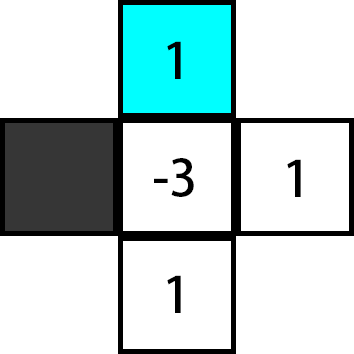
\includegraphics[width=4cm]{Poisson_Stencil}
\centering
\label{fig:PoissonBoundary}
\caption{A finite difference Poisson stencil on the boundary. White cells are interiors cell, i.e. they are degrees of freedom. Blue cell are Dirichlet condition, or essential conditions, that their value are prescribed. Grey cells are exterior cells that are not part of the domain $\Omega$. The face between gray and white cell describes a Nuemann condition, or a nature boundary.}
\end{figure}

But even though we may assume that the boundary conditions are cell aligned at the finest level, this may not holds true for the coarse levels, when the cell size doubles. Figure ~\ref{fig:GeometricCoarsening} demonstrates the heuristic for coarsening boundary conditions. Note that after coarsening, the coarse level discretization may not be of the same order of accuracy to the continuous PDE as the finest level at the boundaries. This inconsistent boundary conditions break the principle that the each level of the multigrid hierarchy should be the discretization of the \textbf{same} continuous PDE. But to compensate this discrepancy, we can introduce additional boundary smoothing to stabilize the multigrid.
\begin{figure}[t]
\centering
\begin{minipage}{.5\textwidth}
  \centering
  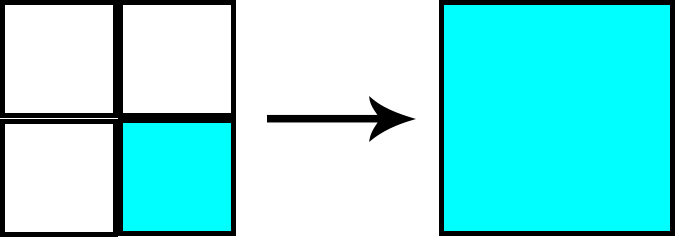
\includegraphics[width=.8\linewidth]{Dirichlet_Coarsening}
\end{minipage}%
\begin{minipage}{.5\textwidth}
  \centering
  
\includegraphics[width=.8\linewidth]{Nuemann_Coarsening}
\end{minipage}
  \caption{Geometric coarsening of the simulation domain. Left: if one of the cells is Dirichlet cell, we will coarsen it as Dirichlet cell at the coarse level, Right: otherwise if one of the cells is interior cell, we will coarsen it as interior cell at the coarse level}
  \label{fig:GeometricCoarsening}
\end{figure}
\section{Garlerkin Coarsening}
Galerkin coarsening, also sometimes refers to algebraic coarsening, is usually the preferred method for handling complex geometries or heterogeneous domains. It was summarized in work [\cite{brandt1986algebraic}]. Many algebraic algorithms, assumes only the top level linear operator is available in matrix form. In such case, the first step of the algorithm is to select the coarse grid DOF based on the matrix given. In this dissertation, we choose the coarsened DOF the same way as in geometric multigrid, that is, coarse DOF coincide with every other fine DOF in each dimension. If readers are interested in the coarse grid selection, I will direct to work [\cite{vanvek1996algebraic}][\cite{brandt1986algebraic}].

After the coarse grid selection, a \textbf{prolongation} operator is constructed. It is a linear operator that interpolates fine DOF values from coarse DOF. The most common prolongation operator is multi-linear interpolation. In 1D, it can be illustrated as Figure~\ref{fig:MultilinearInterpolation}.
\begin{figure}[t]
\centering
\includegraphics[width=6cm]{Interpolation}
  \caption{Multilinear prolongation operator in 1D. The value from corresponding fine nodes is copied from the coarse node, it they coincide in the domain, otherwise the fine node value is interpolated from the two closest coarse nodes each with weight 0.5.}
  \label{fig:MultilinearInterpolation}
\end{figure}

We can also write this in matrix form:
$$
\mathbf{P} = \begin{bmatrix}
1 & 0 & 0 \\
0.5 & 0.5 & 1 \\ 
0 & 1 & 0 \\
0 & 0.5 & 0.5 \\
0 & 0 & 1
\end{bmatrix}
$$
The interpolation process is then:
\begin{equation}
\mathbf{u}^f = \mathbf{P} \mathbf{u}^c
\end{equation}
Here $\mathbf{x}^f$ is the fine grid value and $x^c$ is the coarse grid value. In the case of multi-level hierarchy, we can denote the prolongation operator from level $k+1$ to level $k$ as $\mathbf{P}^k$. Therefore:
\begin{equation}
\mathbf{u}^k = \mathbf{P}^k \mathbf{u}^{k+1}
\end{equation}
Here, $P$ is a rank deficient matrix, which means when prolongate from a coarse level to a fine level, the vector at fine level has a higher dimension and is in general not the correct solution of the fine level discretization. Therefore, smoother is the process used to correct this error. This means smoother should be selected based on error that is invisible to coarse grid, and vise versa, coarse grid should correct error mode that hard to reduce by smoother. In the next section we will discuss more this duality.  Multilinear interpolation has proven to be effective prolongation operator for homogeneous and isotropic PDEs[\cite{mcadams2010parallel}][\cite{aanjaneya2017power}][\cite{zhu2010efficient}]. It is also used by geometric multigrid. 

Now we have defined the prolongation operator $\mathbf{P}^k$. The Galerkin coarsening process construct the $k+1$ operator $\mathbf{L}^{k+1}$ as follows:
\begin{equation}
\mathbf{L}^{k+1} = (\mathbf{P}^k)^T \mathbf{L}^{k}\mathbf{P}^k
\end{equation}
The coarse level correction can be written as(for solving $\mathbf{L}\mathbf{u} = \mathbf{f}$):
\begin{align*}
\mathbf{r} &= \mathbf{b} - \mathbf{L}\mathbf{u}_0 \\
\mathbf{b}^c &= \mathbf{P}^T\mathbf{r} \\
\mathbf{u}^c &= (\mathbf{L}^c)^{-1} \mathbf{b}^c \\
\mathbf{u}^* &= \mathbf{u}_0 + \mathbf{P}\mathbf{u}^c\\
\end{align*}
Here, superscript c indicates unknowns and matrices from the coarse grid. $\mathbf{u}_0$ is the current guess of the fine level solution.$\mathbf{u}^*$ is the new guess of the fine level solution after the coarse correction.
\begin{lem}\label{lemma:projection}The coarse grid correction of Galerkin coarsened hierarchy is a projection.\end{lem}
\begin{proof}
This lemma suggests when doing coarse correction twice, the second correction process will create the same result as first one.

If we start with $\mathbf{u}^* = \mathbf{u}_0 + \mathbf{P}\mathbf{u}^c$.
\begin{align*}
\mathbf{r}^* &= \mathbf{b} - \mathbf{L}\mathbf{u}^* \\
\mathbf{b}^{*c} &= \mathbf{P}^T\mathbf{r}^* \\
&= \mathbf{P}^T(\mathbf{b} - \mathbf{L}\mathbf{u}^*) \\
&= \mathbf{P}^T(\mathbf{b} - \mathbf{L}(\mathbf{u}_0 + \mathbf{P}\mathbf{u}^c))\\
&= \mathbf{P}^T(\mathbf{b} - \mathbf{L}\mathbf{u}_0) - \mathbf{P}^T\mathbf{L}\mathbf{P}\mathbf{u}^c \\
&= \mathbf{P}^T\mathbf{r} - \mathbf{L}^c\mathbf{u}^c \\
&= \mathbf{b}^c - \mathbf{b}^c \\
&= 0
\end{align*}
We can see that the second correction process will have $0$ as right hand side, therefore no correction will be produced.
\end{proof}
In general, we have $rank(L^{k+1}) < rank(L^{k})$. Lemma \ref{lemma:projection} implies that the coarse grid correction is projecting the fine solution onto a subspace and solve within the subspace. All the error modes $\mathbf{e}$ that has property $\mathbf{P}\mathbf{e} = \mathbf{0}$ will be invisible to the coarse level, and rely on the smoother for correction.
\section{Multigrid V-cycle}
Now we have constructed the hierarchy, let's take a look at a multigrid V-cycle.
\begin{algorithm}[H]
\caption{Multigrid V-cycle}
\label{alg:vcycle}
\begin{algorithmic}
\STATE $\mathbf{u}^0 = \mathbf{0}$
\STATE $\mathbf{r}^0 = \mathbf{b}^0 - \mathbf{L}^0\mathbf{u}^0$
\WHILE{$|\mathbf{r}^0| < threshold$ || max\_iteration has reached}
	\FOR{i := 0 \TO k - 2}
		\STATE smooth($\mathbf{u}^i,\mathbf{L}^i,\mathbf{b}^i$);
		\STATE $\mathbf{r}^i = \mathbf{b}^i - \mathbf{L}^i\mathbf{u}^i$
		\STATE $\mathbf{b}^{i+1} = (\mathbf{P}^i)^T\mathbf{r}^i $
	\ENDFOR
	\STATE $\mathbf{u}^{k-1} = (\mathbf{L}^{k-1})^T \mathbf{b}^{k-1}$	
	\FOR{i := k - 2 \TO 0}
		\STATE $\mathbf{u}^{i} += \mathbf{P}^i\mathbf{u}^{i+1} $
		\STATE smooth($\mathbf{u}^i,\mathbf{L}^i,\mathbf{b}^i$);		
	\ENDFOR
	\STATE $\mathbf{r}^0 = \mathbf{b}^0 - \mathbf{L}^0\mathbf{u}^0$
\ENDWHILE
\end{algorithmic}
\end{algorithm}
The process of rather straight forward: at each level, first, we reduce errors that are (hopefully) invisible to the coarse grid using a smoother. Then the residual of the remaining error is computed and restricted to the coarse level. This process is repeated until  the bottom level is reached where the problem is small enough to be solved using a direct solver. This coarse level correction is than prolongated to finer levels, then the smoother is applied again until this process reaches the top. The multigrid V-cycle can be repeated until satisfactory convergence is reached or the max number of iterations has reached.

This multigrid iteration has an asymptotic convergence, that is, after enough iterations, the ratio between the residual norm at iteration $k$ and iteration $k+1$ will converge to a constant[\cite{brandt1977multi}]. After introducing the smoother in the next section, I will give a more concrete example on what this asymptotic convergence can be for an ideal problem.
\section{Smoother}
Smoother a generally refer to a class of iterative solvers that use only local information, and the cost of each application is comparable to a matrix multiplication. Common smoothers are (but not restricted to) Jacobi method, Gauss-Seidel method, Richardson iteration, and successive over-relaxation method. As the simplest, I will take Richardson iteration as example. Richardson iteration can be written as(using notations from before):
 \begin{align*}
\mathbf{r} &= \mathbf{b} - \mathbf{L}\mathbf{u}_k \\
\mathbf{u}_{k+1} &= \mathbf{u}_k\mathbf{r} \\
\end{align*}
Here $\mathbf{u}_k$ is the solution at iteration $k$. If we define $\mathbf{u}^*$ the solution, that is
$$
\mathbf{L}\mathbf{u}^* = \mathbf{b}
$$
We can write the error of the current solution  as
$$
\mathbf{e}_k = \mathbf{u}^* - \mathbf{u}_k 
$$
And the residual is then
$$
\mathbf{r}_k = \mathbf{L}\mathbf{e}_k
$$
Assuming $\mathbf{L}$ is symmetric positive definite. We write the Eigen vector of $\mathbf{L}$ as $\mathbf{v}_i$, that are orthogonal to each other. Then we can write the error as combination of the Eigen vectors:
$$
\mathbf{e}_k = \sum_i \gamma_i\mathbf{v}_i
$$
Here $\gamma_i$ are the length when project $\mathbf{e}_k$ onto $\mathbf{v}_i$.
\chapter{A Schur-complement Domain Decomposition Solver for Multi-accelerator Equipped Platform} \label{Chapter:DD}

\section{Multi-accelerator Equipped Platform}
Modern compute platforms for scientific computing are evaluated based on their compute power in FLOPS(FLoating Operation Per Second) and memory bandwidth in GB/s (GibaByte Per Second). A single CPU equipped machine, Intel\textsuperscript{\textregistered} Xeon\textsuperscript{\textregistered} Gold 6150 Processor for example, may have 1.3 TFLOP compute power and 120 GB/s memory bandwidth with maximum of 768GB of memory. While a multi-GPU equipped machine, 4 GTX 1080TI for instance, can have aggregately 44 TFLOP compute power and 1936 GB/s memory bandwidth, but only 44 GB of total memory at the same cost. This 33x compute power and 8x memory bandwidth does not come without any cost. Each accelerator can only operate at peak performance for the data allocated at its own memory. Cross GPU data access or inter CPU/GPU data access are significantly slower not only in terms of bandwidth but also in terms of latency, 16GB/s for PCI-E 3.0, 80 GB/s for NVLink 1.0 and 150 GB/s for NVLink 2.0. A heterogeneous platform often refers to those type of machines that not all resources can be accessed at the same cost across the platform. For instance, a GPU(GTX 1080TI as an example) may be able to access data allocated on its own memory at 484GB/s, but for accessing data allocated on CPU, it would require communication across PCI-E at maximum speed 16GB/s with couple of microsecond latency. 

\begin{figure}[t!]
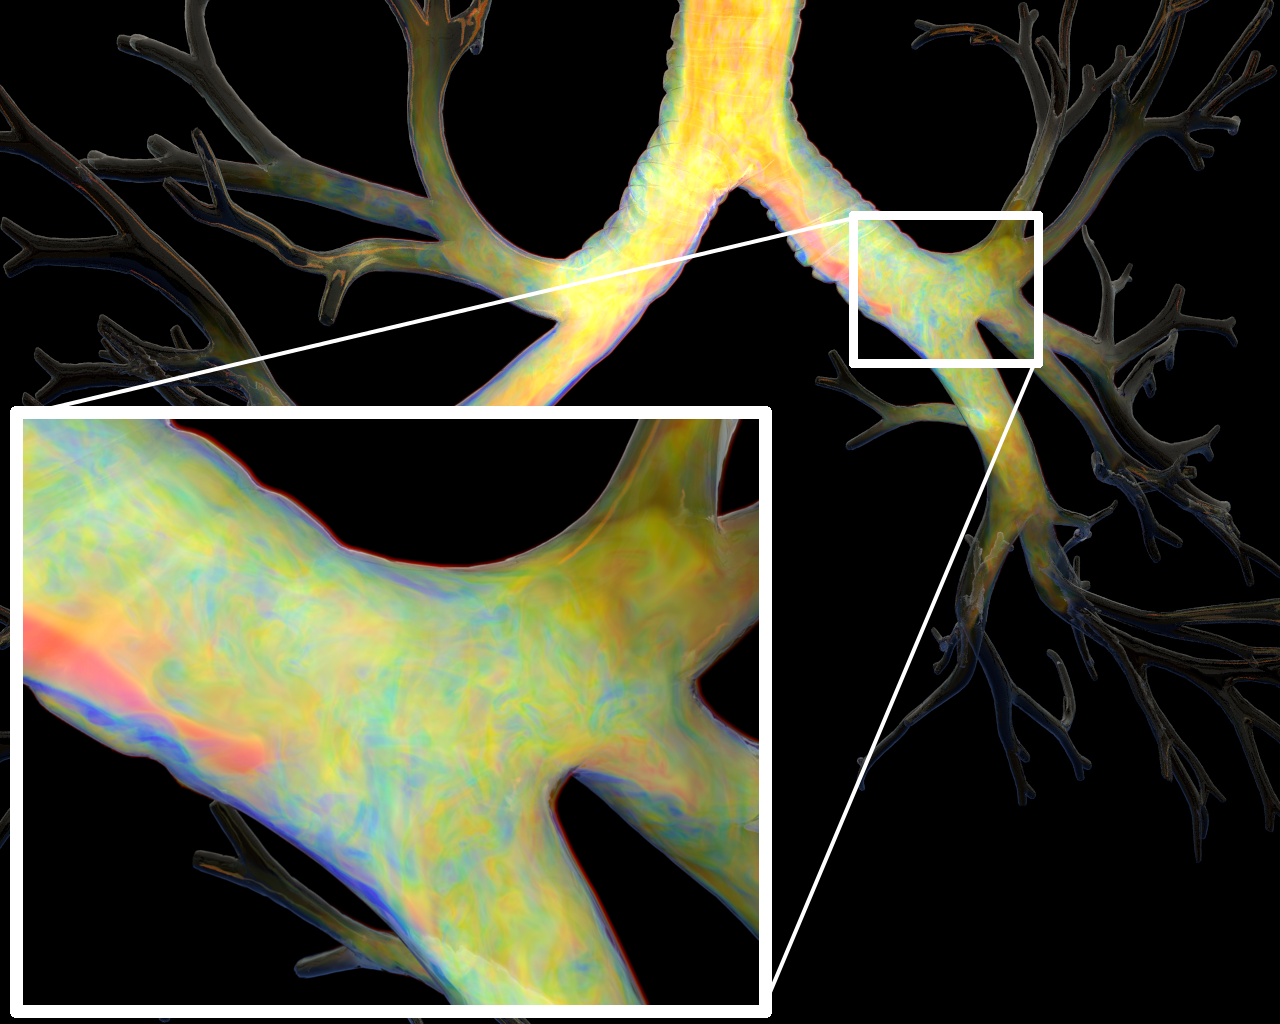
\includegraphics[height=.4\textwidth]{images/DD/Teaser_Part1.png}
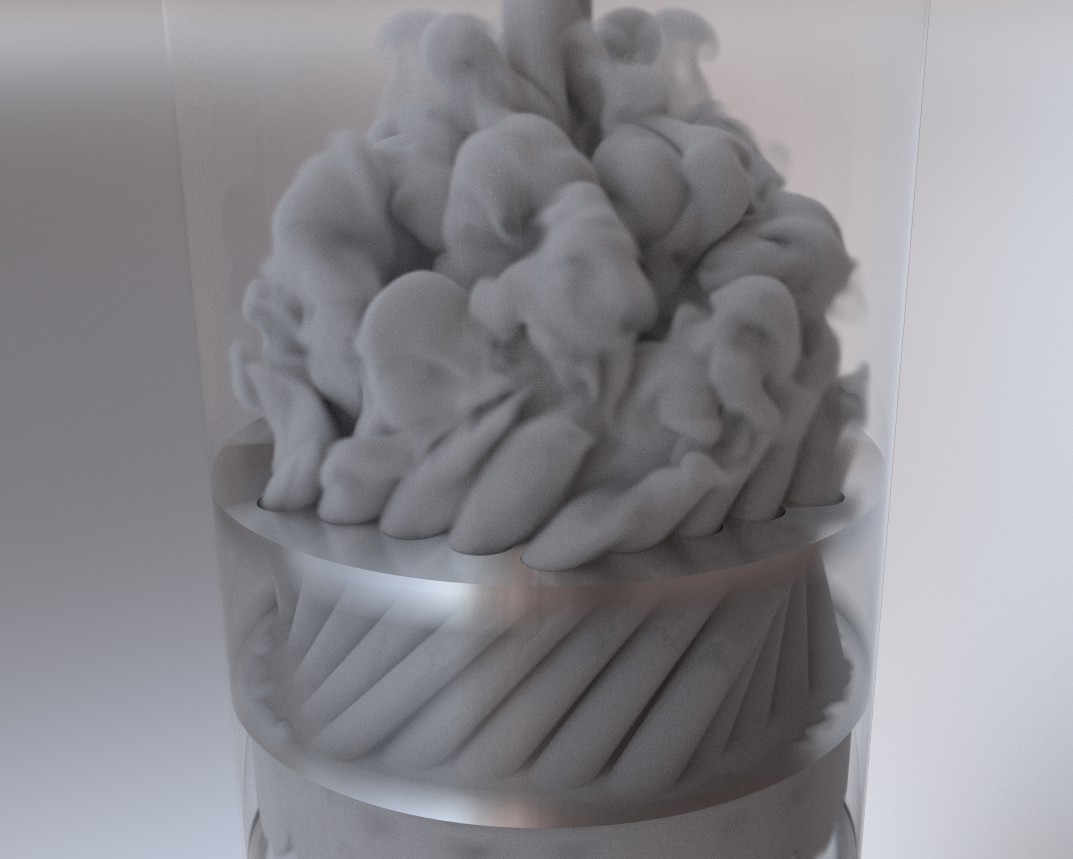
\includegraphics[height=.4\textwidth]{images/DD/Teaser_Part2_5x4.png}
%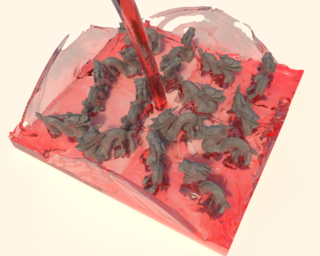
\includegraphics[width=.33\textwidth]{images/teaser_dragon_splash.png}
%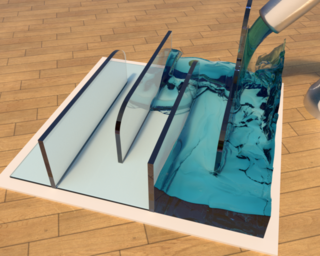
\includegraphics[width=.33\textwidth]{images/teaser_snake_channel.png}
%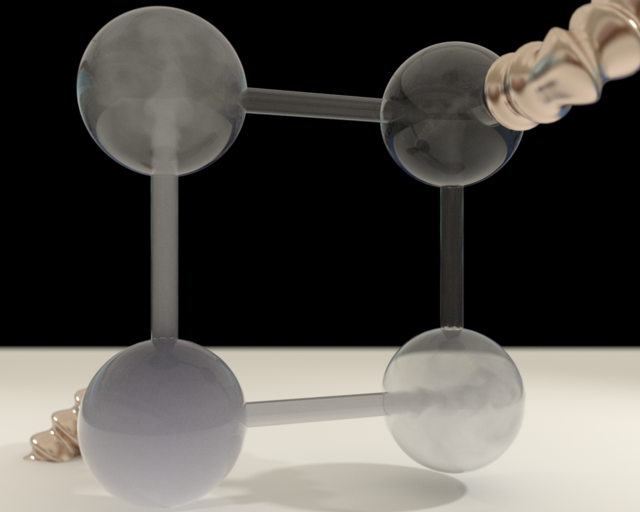
\includegraphics[width=.33\textwidth]{images/teaser_flasks.png}
\caption{Left: Smoke injected into a model of the bronchi. Color illustrates vorticity magnitude. Simulation contains 1.8 billion active cells, sparsely
  occupying a $8192^2\!\times\!4096$ background grid. Right: Smoke injected from the bottom of a cylinder, and forced through a metal gasket (rendered semi-transparent) with a
  twisted bundle of cylindrical holes. Total of 1.2 billion active cells, in a $1024^2\!\times\!2048$ background grid.}
\label{fig:DD-teaser}
\end{figure}

When designing algorithms for a heterogeneous platform, the locality of data need always be kept in mind for best utilization of the computing resources, otherwise, in the most unfortunate case, only a memory speed of 16GB/s maybe utilized, instead of the ideal 1936 GB/s. In such a case, the single CPU platform with 140 GB/s memory bandwidth may better perform this multi-GPU equipped machine. It should be noted that this non-uniformity of bandwidth is not an aberration of hardware design that is likely going away; in fact it is consistent with the fact that memory
hierarchies, and physical proximity of memory to computational units, have long given rise to differentiation in latency and bandwidth between different parts of the computational
platform.

Unfortunately, some of the best performing solvers (in terms of convergence efficiency) such as multigrid are the cases of the worst scenarios. The building blocks of a multigrid
solver, namely the smoothing routine and transfer operators, require global synchronization after their execution while carrying out only a very modest amount of useful computation
in between synchronization points. In particular, a Jacobi or Gauss-Seidel style smoother requires no more than two passes over the data in memory, which completes in a very small
fraction of the cost incurred for transferring the data to the GPU card, or out of it upon completion. Of course, one could take the opportunity to carry out several smoothing
iterations per offload operation; however, without synchronization at partition boundaries this extra effort will hardly translate to worthwhile gains in convergence. As a result,
the benefit of the GPU offload is negated, and such large problems are better off being solved homogeneously on the CPU. Although there might be room for implementation refinements
and adaptation of multigrid paradigms to curb this overhead, we are not aware of prior work that has demonstrated viability of a GPU-offload paradigm for multigrid solvers, when
the problem size exceeds the memory capacity of the GPU card(s), compare to a well-optimized CPU implementation. Our proposed approach directly addresses this challenge: instead of
executing just a few iterations of a smoother routine, we run an entire solver routine on the GPU for each independent subdomain we offload to it. In our case, that extra effort
does translate to accelerated convergence, and the GPU computation is long enough to absorb the transfer cost.
\section{Domain Decomposition as Divide-and-conquer}
In this chapter, a Schur Complement domain decomposition method is presented, the objective is to demonstrate an effective, and hopefully inspiring adaptation to fluids simulation of a class of numerical techniques that has received much more exposure in scientific computing than graphics research. We note, however, that Schur Complement methods provide a general framework, and not just a singular algorithm; in fact, similar to multigrid methods, careful variations from the general algebraic theme make all the difference between a given scheme being highly effective or underwhelming for a specific application. In this vein, we consciously restricted the scope of our investigation to just uniform discretizations of fluids, specifically targeted the Poisson equation (although our formulations should readily extend to elasticity, or other elliptic problems), and did not emphasize the implications of heterogeneous computing to other parts of the fluid simulation pipeline.

The classical divide-and-conquer paradigm encountered in combinatorial algorithms often presumes building blocks that accurately solve subsets of the overall problem. In our numerical context, one of the key opportunities we will exploit is the option to design what is not an exact solver, but an excellent approximation of one, and subsequently use it as a preconditioner. In this context, we will adopt a slightly different standard which we will design our ``inaccurate'' divide-and-conquer scheme to satisfy. Our building block will be an inexact solver for the Poisson equation on independent partitions of our domain, which is however of good enough quality to be used as an excellent Conjugate Gradients preconditioner (i.e. it would lead to convergence in a small number of iterations, that does not significantly increase as the subdomain size grows larger). Subsequently, our objective would be to combine such ``nearly accurate'' building blocks into a global approximate solver that meets the same benchmark, i.e. it can be used as a highly effective preconditioner that allows CG to converge in a comparably small number of iterations as its individual constituents. We note that,short of this standard, using divide-and-conquer tricks can be a slippery slope and result is significantly degraded performance.

\section{The classic Schur complement method}
\label{sec:dd-fundamentals}

We introduce the basic principles of the Schur complement method [\cite{quarteroni:1999:domain}] by explaining how an aggregate solver for the pressure Poisson
equation can be assembled using as subroutines two independent solvers for two non-overlapping partitions of the entire computational domain.
After covering the basic theory we will detail how this construction extends to multiple partitions, and derive a preconditioner based on this concept in later sections.

\subsection{The two-subdomain case}

\begin{wrapfigure}{r}{.25\columnwidth}
\mbox{
  \begin{overpic}[width=.3\columnwidth]{images/DD/two_subdomains.pdf}
    \put(15,15){$\Omega_1$}
    \put(60,50){$\Omega_2$}
    \put(82,8){$\Gamma$}
  \end{overpic}}
\end{wrapfigure}
Consider a domain $\Omega$ that has been partitioned into two subdomains
$\Omega_1$ and $\Omega_2$ through an interface region $\Gamma$. Let us assume we have a
finite-difference discretization of the pressure Poisson equation on $\Omega$,
and that the interfacial region $\Gamma$ is thick enough to shield any stencil in $\Omega_1$ from including a point in $\Omega_2$ (and vice-versa).  In
practice, when using the standard $7$-point stencil in a Cartesian discretization, the interface layer $\Gamma$ can simply be one-node thick as long as it cleanly
decouples $\Omega$ into two distinct subdomains (although $\Gamma$ could also be made wider, if desired). For simplicity of notation we will write the Poisson
equation as $Ax=b$, with the understanding that the vector $x$ contains the unknown pressure values and $b$ contains the respective divergence values of the velocity
field. We then reorder degrees of freedom as:
% to group together degrees of freedom in $\Omega_1$, $\Omega_2$ and $\Gamma$ as follows:
%When solving the Poisson equation $Ax=b$ on $\Omega$, if the degrees of freedom have been reordered such that
\begin{eqnarray}
\label{eqn:dof}
x=
\begin{bmatrix}
x_1 \\
x_2 \\
x_\Gamma
\end{bmatrix}
,\enspace\enspace\enspace\enspace
b=
\begin{bmatrix}
b_1 \\
b_2 \\
b_\Gamma
\end{bmatrix}
\end{eqnarray}
where $x_i,b_i$ correspond to values in $\Omega_i$, for $i\in\{1,2\}$ (and similarly $x_\Gamma,b_\Gamma$ correspond to degrees of freedom in $\Gamma$). Under this
reordering, the matrix $A$ assumes the following block form:
\begin{eqnarray}
\label{eqn:block-sparsity-A}
A=
\begin{bmatrix}
A_{11} & & A_{1\Gamma} \\
& A_{22} & A_{2\Gamma} \\
A_{\Gamma 1} & A_{\Gamma 2} & A_{\Gamma\Gamma}
\end{bmatrix}
\end{eqnarray}
Note that due to symmetry of $A$, we have $\varB{A}_{\Gamma 1}^T\!\!=\!\!\varB{A}_{1\Gamma}$ and $\varB{A}_{\Gamma 2}^T\!\!=\!\!\varB{A}_{2\Gamma}$ for the off-diagonal blocks.
Using this block form of $A$ it is possible to write the following factorization of the \emph{inverse} matrix $A^{-1}$:
\begin{eqnarray*}
\label{eqn:block-factorization-A}
\varB{A}^\varA{-1}\!=\!\!
\begin{bmatrix}
I & & \varB{-A}_{11}^\varA{-1}A_{1\Gamma} \\
& I & \varB{-A}_{22}^\varA{-1}A_{2\Gamma} \\
\ \ \ \tikzmark{c1} & & \ \ \ \ I\ \ \ \ \tikzmark{c2}
\end{bmatrix}
\hspace{-.2cm}
\begin{bmatrix}
\!A_{11}^\varA{-1}\!\!\! & & \\
& \!\!\!\!A_{22}^\varA{-1}\!\! & \\
\!\tikzmark{d1} & & \!\!\!\Sigma^\varA{-1}\!\tikzmark{d2}
\end{bmatrix}
\hspace{-.2cm}
\begin{bmatrix}
I & & \\
& I & \\
\tikzmark{ct1}\varB{-A}_{\Gamma 1}A_{11}^\varA{-1} & \varB{-A}_{\Gamma 2}A_{22}^\varA{-1} & I\tikzmark{ct2}
\end{bmatrix}
\begin{tikzpicture}[overlay, remember picture,decoration={brace,amplitude=5pt}]
\draw[decorate,thick] (c2.south) -- (c1.south)
      node [midway,below=5pt] {$U$};
\draw[decorate,thick] (d2.south) -- (d1.south)
      node [midway,below=5pt] {$D$};
\draw[decorate,thick] (ct2.south) -- (ct1.south)
      node [midway,below=5pt] {$U^T$};
\end{tikzpicture}
\end{eqnarray*}

where
$$\Sigma=A_{\Gamma\Gamma}-A_{\Gamma 1}A_{11}^\varA{-1}A_{1\Gamma}-A_{\Gamma 2}A_{22}^\varA{-1}A_{2\Gamma}$$
is the \emph{Schur complement} of the block $A_{\Gamma\Gamma}$ in equation (\ref{eqn:block-sparsity-A}).
The validity of this factorization can be verified via a direct substitution into the identity $A\!\cdot\!A^{-1}\!=\!I$.
 Finally, since $A$ (and its inverse) is a symmetric positive definite(SPD) matrix, this factorization
implies that the Schur complement is also symmetric and positive definite (the matrix $D$ is equal to the symmetric conjugation of the symmetric positive definite
matrix $A^{-1}$ with the matrix $U^{-1}$; hence its diagonal sub-block $\Sigma^{-1}$ is symmetric definite, too).

\begin{figure*}[h]
\tiny
\begin{align}
\label{eqn:factorization-k-subdomains-exact}
\hspace{-3cm} A^\varA{-1} &=
\begin{bmatrix}
I & & & \varB{-A}_{11}^\varA{-1}A_{1\Gamma} \\
& \ddots & & \vdots \\
& & I & \varB{-A}_{kk}^\varA{-1}A_{k\Gamma} \\
& & & I
\end{bmatrix}
\begin{bmatrix}
A_{11}^\varA{-1} & & & \\
& \ddots & & \\
& & A_{kk}^\varA{-1} & \\
& & & \Sigma^\varA{-1}
\end{bmatrix}
\begin{bmatrix}
I & & & \\
& \ddots & & \\
& & I & \\
\varB{-A}_{\Gamma 1}A_{11}^\varA{-1} & \ldots & \varB{-A}_{\Gamma k}A_{kk}^\varA{-1} & I
\end{bmatrix} \\
\label{eqn:factorization-k-subdomains-five}
&=
\begin{bmatrix}
A_{11}^\varA{-1} & & & \\
& \ddots & & \\
& & A_{kk}^\varA{-1} & \\
& & & I
\end{bmatrix}
\begin{bmatrix}
I & & & \varB{-A}_{1\Gamma} \\
& \ddots & & \vdots \\
& & I & \varB{-A}_{k\Gamma} \\
& & & I
\end{bmatrix}
\begin{bmatrix}
A_{11} & & & \\
& \ddots & & \\
& & A_{kk} & \\
& & & \Sigma^\varA{-1}
\end{bmatrix}
\begin{bmatrix}
I & & & \\
& \ddots & & \\
& & I & \\
\varB{-A}_{\Gamma 1} & \ldots & \varB{-A}_{\Gamma k} & I
\end{bmatrix}
\hspace{-.2cm}
\begin{bmatrix}
A_{11}^\varA{-1} & & & \\
& \ddots & & \\
& & A_{kk}^\varA{-1} & \\
& & & I
\end{bmatrix} \\
\label{eqn:factorization-k-subdomains-approx-five}
&\approx
\begin{bmatrix}
\textcolor{red}{A_{11}^\dagger} & & & \\
& \ddots & & \\
& & \textcolor{red}{A_{kk}^\dagger} & \\
& & & I
\end{bmatrix}
\hspace{-.2cm}
\begin{bmatrix}
I & & & \varB{-A}_{1\Gamma} \\
& \ddots & & \vdots \\
& & I & \varB{-A}_{k\Gamma} \\
& & & I
\end{bmatrix}
\hspace{-.2cm}
\begin{bmatrix}
I & & & \\
& \ddots & & \\
& & I & \\
& & & \textcolor{red}{\Sigma^\dagger}
\end{bmatrix}
\hspace{-.15cm}
\left\{
I+
\begin{bmatrix}
& & & \\
& & & \\
& & & \\
\varB{-A}_{\Gamma 1} & \ldots & \varB{-A}_{\Gamma k} & I
\end{bmatrix}
\hspace{-.2cm}
\begin{bmatrix}
\textcolor{red}{A_{11}^\dagger} & & & \\
& \ddots & & \\
& & \textcolor{red}{A_{kk}^\dagger} & \\
& & & I
\end{bmatrix}
\right\}
\end{align}
\normalsize
\end{figure*}

\subsection{The multiple subdomain solver}
\begin{figure*}[t!]
\includegraphics[width=\textwidth]{images/DD/SolverStages.pdf}
\caption{Illustration of the core concept of our method: (b) We split the computational grid into subdomains, and independently solve them on the GPU(s), using
  zero Dirichlet conditions on subdomain boundaries. (c) Fluxes of the subdomain solutions are computed and sent to 
  the CPU. (d) A specially formulated system is solved on the interface, using the CPU. This produces the exact value of the interface variables. (e) Those
  values are sent to the subdomains, and set as Dirichlet conditions. (e) A final subdomain solve on the GPU yields the global solution.}
\label{fig:pipeline}
\end{figure*}
This formulation extends naturally to an arbitrary number of $k$ subdomain partitions $\Omega_1,\ldots,\Omega_k$ separated by an interface set $\Gamma$ (figure
\ref{fig:pipeline} depicts such a partitioning into four subdomains, with the interface $\Gamma$ highlighted as the magenta-colored separator surface). The
corresponding factorization of $A^{-1}$ in this case is given in equation (\ref{eqn:factorization-k-subdomains-exact}). In order to translate this algebraic expression
into a solver algorithm, we first re-factor this into the five-matrix product of equation (\ref{eqn:factorization-k-subdomains-five}), which has every subdomain
inverse $A_{ii}^\varA{-1}$ appear only twice (as opposed to three inversions per subdomain, in equation \ref{eqn:factorization-k-subdomains-exact}). The last
algebraic manipulation, as given in equation (\ref{eqn:factorization-k-subdomains-approx-five}) further avoids the appearance of the subdomain Laplacian
$A_{ii}$, requiring only the inverses of such matrices. In this expression we have also substituted the symbol ${\color{red}M^\dagger}\approx M^{-1}$ for
\emph{approximate} inverses of $A_{ii}$ and $\Sigma$. If the \emph{exact} inverse of these matrices was used, equation (\ref{eqn:factorization-k-subdomains-approx-five})
becomes identically equal to the five-factor expression of equation (\ref{eqn:factorization-k-subdomains-five}). We will later engage in such approximations; for now, we
may assume that all these inverses are exact.  


%  The reader is
% welcome to verify the accuracy of this factorization via simple algebraic
% substitution. Since the matrix $A$ is symmetric and positive-definite (and hence, $A^\varA{-1}$),
% it follows from the factorization that the matrix $D$ is symmetric and positive-definite. 
% The symmetry and positive-definiteness of the matrix $\Sigma$ now follows from
% the fact that both the matrices $A_{11}$ and $A_{22}$ are symmetric and positive-definite.
% Equivalently, $A^\varA{-1}$ can also be factorized as $A=C'D'C'^T$, where

% \begin{eqnarray*}
% \label{eqn:equivalent-block-factorization-A}
% C'=
% \begin{bmatrix}
% A_{11}^\varA{-1} & & \\
% & A_{22}^\varA{-1} & \\
% & & I
% \end{bmatrix}
% \hspace{-.2cm}
% \begin{bmatrix}
% I & & \varB{-A}_{\Gamma 1} \\
% & I & \varB{-A}_{\Gamma 2} \\
% & & I
% \end{bmatrix}, \enspace\enspace
% D'=
% \begin{bmatrix}
% I & & \\
% & I & \\
% & & \Sigma^\varA{-1}
% \end{bmatrix}
% \end{eqnarray*}
% This factorization only requires computation of
% the inverses $A_{11}^\varA{-1}$ and $A_{22}^\varA{-1}$ for the individual subdomains.
% Multiplying the vector $b$ from equation (\ref{eqn:dof}) with
% this factorization
% from right to left yields the following algorithm for solving the original system
% $Ax=b$:

The Schur complement method effectively solves the equation $Ax=b$ by multiplying the right hand side $b$ with the factorized equivalent of $A^{-1}$ from equation 
(\ref{eqn:factorization-k-subdomains-approx-five}). The key observation is that we can apply this multiplication indirectly, without explicitly constructing the
matrix in this factorization. We do this as follows:
\vspace*{-.15in}
\begin{enumerate}
\item
Solve $k$ subproblems: $A_{11}\hat x_1=b_1$, \ldots,  $A_{kk}\hat x_k=b_k$.
\vspace*{-.05in}
\item
Solve $\Sigma x_\Gamma=b_\Gamma-A_{\Gamma 1}\hat x_1-A_{\Gamma 2}\hat x_2 - \ldots -A_{\Gamma k}\hat x_k $.
\vspace*{-.05in}
\item
Solve the $k$ new subproblems\\ $A_{11}\delta x_1=-A_{1\Gamma}x_\Gamma$, \ldots, $A_{kk}\delta x_k=-A_{k\Gamma}x_\Gamma$.
\vspace*{-.05in}
\item
Update $x_1\leftarrow \hat x_1+\delta x_1$, \ldots, $x_k\leftarrow \hat x_k+\delta x_k$.
\end{enumerate}
Observe that steps ($1$) and ($3$) require the solution of fully decoupled systems for each subdomain $\Omega_i$, and this can easily be performed in
parallel without any need for communication or synchronization.
Step ($2$) requires the solution of a symmetric and positive definite system (with the Schur complement $\Sigma$ as the
coefficient matrix). Traditionally, solvers based on this method attempt to solve this interface system using a preconditioned Krylov
subspace method such as Conjugate Gradients. We will deviate from
this practice, and use equation (\ref{eqn:factorization-k-subdomains-approx-five}) instead, to design a preconditioner for the \emph{global} (coupled) system.

 It is important to examine the algebraic structure of $\Sigma$, and assess the performance implications of attempting to solve the system in step (2) directly.
 For a volumetric
domain $\Omega$ with $N$ total degrees of freedom, the dimensionality of $\Gamma$ would be $O(\sqrt{N})$ in 2D, and $O(N^{2/3})$ in 3D. Note, however, that in contrast to the
sparse Laplace matrix $A$, the Schur complement is a dense matrix, thus having $O(N^{4/3})$ entries and requiring at least as much computation to solve. Asymptotically, this would
make step (2) above by far the bottleneck of the solver, if $\Sigma$ was to be explicitly constructed. Furthermore, the construction of the matrix alone would likely require even
more computation, as it would need to account for computing the subdomain inverses $A_{ii}^\varA{-1}$. Using Conjugate Gradients as the solver in step (2) opens up an interesting
possibility: the CG algorithm does not need an explicitly constructed matrix $\Sigma$, as long as we have a way to compute matrix-vector products $\Sigma x_\Gamma$. In turn, this
would require computing products of the form $A_{\Gamma i}A_{ii}^\varA{-1}A_{i\Gamma}x_\Gamma$ as efficiently as possible. Although the factors $A_{\Gamma i}$, $A_{i\Gamma}$ are
sparse enough to allow efficient multiplication, multiplying with $A_{ii}^\varA{-1}$ (i.e. solving a subdomain Poisson problem) requires at least linear cost relative to the size
of the subdomain (assuming a linear-complexity solver, like an extremely well built multigrid scheme, iterated to full convergence). There would be opportunity for parallelization
across subdomains, but we would be still confronted with a linear complexity cost for \emph{each} CG iteration, and we would have to rely on constructing an extremely efficient
preconditioner to ensure that only a small finite number of iterations would suffice, independent of resolution. Nevertheless, this is the
  path followed by many derivative techniques
of the Schur complement method (often referred to as \emph{iterative substructuring}; an excellent synopsis of such options is given in the classic book by \cite{quarteroni:1999:domain}).


\section{A Schur-complement preconditioner}
\label{sec:schur-complement-preconditioner}

In light of the challenges detailed in section~\ref{sec:dd-fundamentals} we propose certain strategic simplifications that would make the Schur complement method
yield an approximate solver of the Poisson equation, rather than a strictly accurate one. Our intent would be to use this approximation as a preconditioner for the
Conjugate Gradients method, applied to the full-scale Poisson problem. Our last transformation of the factorized form for $A^{-1}$, captured in equation
(\ref{eqn:factorization-k-subdomains-approx-five}) was precisely intended to facilitate this process. We can easily show that any \emph{nonsingular} approximation
$A_{ii}^\dagger\approx A_{ii}^{-1}$ of the subdomain inverses, combined with a \emph{symmetric positive definite (SPD)} approximation $\Sigma^\dagger\approx\Sigma^{-1}$
will produce, after substitution in equation
(\ref{eqn:factorization-k-subdomains-approx-five}), a symmetric and positive definite matrix approximation to
$A^{-1}$. Thus multiplication with this expression can be used as a preconditioner for the Conjugate Gradients method.
% We will design these approximations so that
%they offer the best approximation that can be afforded while being highly suitable for parallel implementation on a heterogeneous computing platform.  

%To cater to the observations made in section~\ref{sec:dd-fundamentals},
%we pursue instead to create the approximate inverse shown in equation (\ref{eqn:factorization-k-subdomains-approx-five}) which can be used as a high efficiency preconditioner for a
%Krylov subspace method such as conjugate gradients.
%Here, $A_{ii}^\dagger$ is an approximation to $A_{ii}^\varA{-1}$, for
%$i\in\{1,\ldots,k\}$, and $\Sigma^\dagger$ is an approximation to $\Sigma^\varA{-1}$.
%The only restriction imposed on this matrix to be used as a preconditioner is
%that $A_{11}^\dagger,\ldots,A_{kk}^\dagger,\Sigma^\dagger$ should be symmetric
%and positive-definite, which would guarantee that the entire preconditioner is
%symmetric and positive-definite.

From an implementation standpoint, we map the application of this preconditioner to a heterogeneous platform by assigning the interior degrees of freedom of each
subdomain $\Omega_i$ to a single GPU or Many-Core accelerator card, while the interface degrees of freedom ($\Gamma$) will be the maintained on the CPU. We design
the approximate subdomain inverses $A_{ii}^\dagger$ so that they can be multiplied with respective vectors exclusively on the GPU, local to the accelerator that owns
the subdomain $\Omega_i$. Multiplication with the matrix blocks $A_{\Gamma i}$ will coincide with data transfer from the card that owns $\Omega_i$ to the CPU, while
multiplication with the transpose $A_{i\Gamma}$ will relay data from the CPU to the respective accelerator in the opposite direction. Multiplication with the
approximate inverse of the Schur complement, i.e. $\Sigma^\dagger$, will be handled fully on the CPU. The application of this preconditioner is formalized in
pseudocode in Algorithm 1.  

%Our intent is to apply this preconditioner in a distributed fashion using both
%CPU and available GPUs on our system. In the context of the conjugate
%gradient method, the factorization in equation (\ref{eqn:factorization-k-subdomains-approx-five})
%is never required to be computed explicitly, only its action
%$(z_1,\ldots,z_k,z_\Gamma)^T$ is needed on the residual vector $(r_1,\ldots,r_k,r_\Gamma)^T$.
%The spirit of our method is to perform all computations associated with
%$A_{ii}^\dagger$ on the GPU, those associated with $\Sigma^\dagger$
%on the CPU, and the operators $A_{i\Gamma},A_{\Gamma i}$ are emulated
%by transfer operations from the CPU to the GPU, where $i\in\{1,\ldots,k\}$.
%Algorithm~\ref{alg:apply-preconditioner} illustrates the implementation.

\begin{algorithm}{h}
\caption{Preconditioner application $\boldsymbol{z}=A^\dagger\boldsymbol{r}$, from eqn. (\ref{eqn:factorization-k-subdomains-approx-five})}
\label{alg:apply-preconditioner}
\begin{algorithmic}[1]
\FOR{$i=1\ldots k$}
\STATE\COMMENT{In parallel, on GPU}
\STATE {Get $r_i\leftarrow$ CPU}
\STATE {Solve $q_i\leftarrow A_{ii}^\dagger r_i$}
\STATE {Compute $s_\Gamma^{(i)}\leftarrow -A_{\Gamma i}q_i$}
\STATE {Send $s_\Gamma^{(i)}\rightarrow$ CPU}
\STATE {Send $q_i\rightarrow$ CPU}
\ENDFOR
\STATE Compute $f_\Gamma=r_\Gamma+s_\Gamma^{(1)}+\ldots+s_\Gamma^{(k)}$\COMMENT{on CPU}
\STATE Solve $z_\Gamma\leftarrow\Sigma^\dagger f_\Gamma$
\FOR{$i=1\ldots k$}
\STATE\COMMENT{In parallel, on GPU}
\STATE {Get $q_i\leftarrow$ CPU}
\STATE Get $z_\Gamma\leftarrow$ CPU
\STATE Compute $f_i\leftarrow -A_{i\Gamma}z_\Gamma$
\STATE Solve $z_i\leftarrow A_{ii}^\dagger f_i$
\STATE Add $z_i+=q_i$
\STATE {Send $z_i\rightarrow$ CPU}
\ENDFOR
\end{algorithmic}
\end{algorithm}

\subsection{Multigrid subdomain solver}

For approximating $A_{ii}^\dagger$ in the formulation described above, we use a simple, voxel-accurate multigrid solver in the spirit
similar to prior works
\cite{mcadams2010parallel,Molemaker:2008:LowViscosityFlow},
with some embellishments to support sparsely populated domains as
discussed in section \ref{sec:implementation-details}. The multigrid hierarchy is constructed by classifying every grid
cell as ``interior'', ``exterior'' (to the active domain) or ``Dirichlet'', and coarsening this classification to voxels of lower resolution grids. Trilinear
transfer operators and a damped Jacobi smoother are employed, with an additional
smoothing effort devoted to a narrow band around the boundary (3-7
iterations) for each interior smoothing pass.



\section{The interface Schur-complement system}
\label{sec:sigma-solver}

The last remaining piece for generating our preconditioner is the design of the approximation $\Sigma^\dagger$ and the application of its effective numerical
solution which is hosted exclusively on the CPU. As previously stated, our objective is to arrive at an algorithm that is sublinear in complexity relative to the
size of the overall boundary and yields a good approximation to the exact matrix
$\Sigma=A_{\Gamma\Gamma}-\sum_{i=1}^kA_{\Gamma i}A_{ii}^\varA{-1}A_{i \Gamma}$.
\changed
{The approximations incurred in $\Sigma^\dagger$ are twofold: (a) instead of solving $\Sigma x_\Gamma=b_\Gamma$ exactly, we will substitute a number of V-cycles of an
  appropriately designed multigrid scheme, and (b) we modestly modify the matrix used in this multigrid scheme, using adaptivity, to reduce the cost of direct algebra.}
{We will solve the approximate system $\Sigma^\dagger x_\Gamma=b_\Gamma$ using a multigrid method, which will avoid forming the dense matrix $\Sigma^\dagger$
explicitly. Furthermore, we will leverage adaptive coarsening of the subdomains to reduce the dimensionality of the direct algebra involved in our manipulations.}

\begin{figure}[t!]
\begin{center}
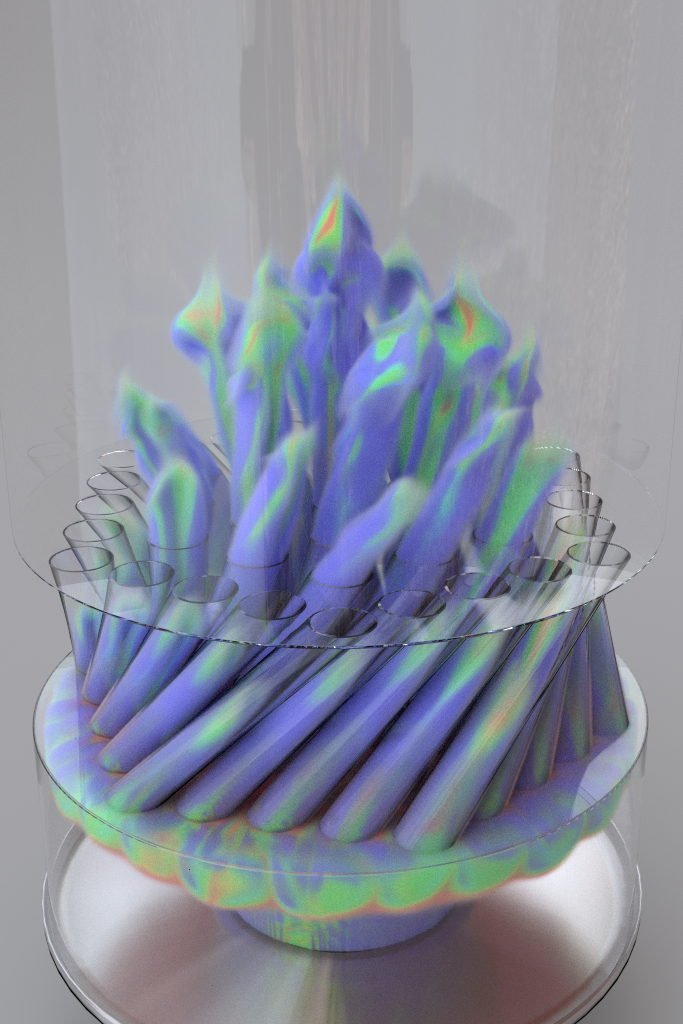
\includegraphics[width=.49\columnwidth]{images/DD/sieve_smoke_150_alternate.png} 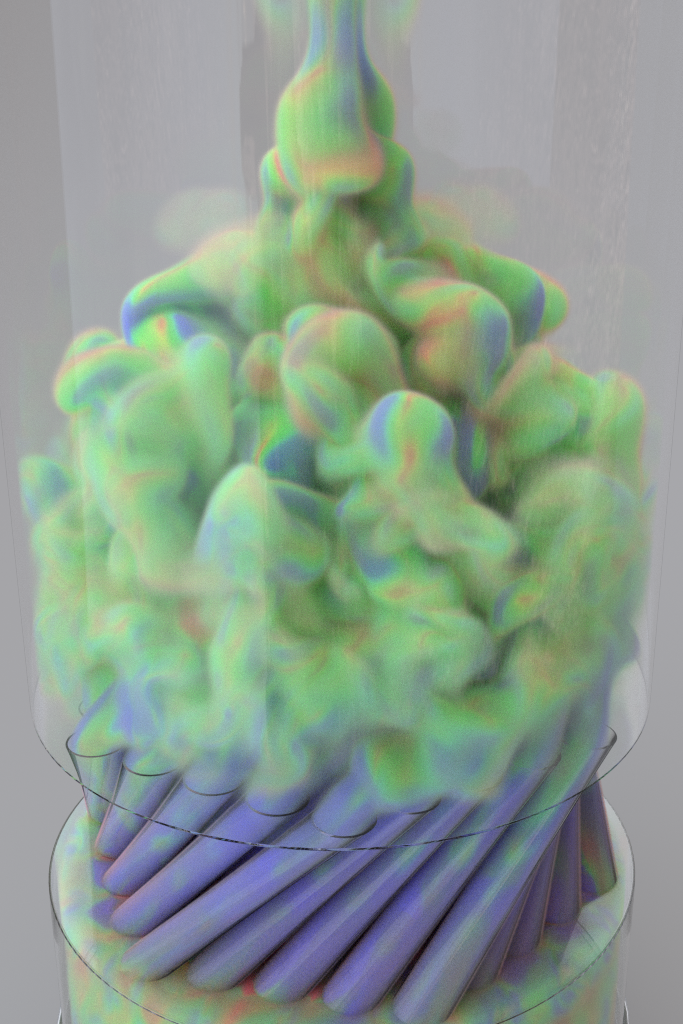
\includegraphics[width=.49\columnwidth]{images/DD/sieve_smoke_255_alternate.png}
\end{center}
\caption{Smoke injected from the bottom of a cylinder, and forced through a
  twisted bundle of cylindrical holes. Color corresponds to vorticity magnitude. Total 1.2B active cells, in a $1024^2\!\times\!2048$ grid.}
\label{fig:sieve}
\end{figure}


\subsection{Multigrid solver for the interface}
\label{sec:interface-multigrid-solver}

The Schur complement matrix $\Sigma$ is not only symmetric and positive definite, but it can further be shown that it is an \emph{elliptic} operator, as it is a
discretization of the continuous and elliptic \emph{Steklov-Poincar\'{e} operator} for the Poisson equation~[\cite{Smith:1996:DDP:238150}]. This suggests that a
multigrid solver (on the interface variables; separate from the multigrid cycles used to approximate the subdomain inverses) could be applicable.
%For such a multigrid scheme, we need a hierarchy of discretizations, a smoother, and appropriate transfer operations.
 The simplest technique for building the multigrid
hierarchy is to use Galerkin coarsening to construct the operator at each
resolution level. However, we do not pursue this option as it requires explicitly computing
the matrix $\Sigma$ at the finest level, which is a computationally expensive proposition. We propose a different conceptual construction of the operator hierarchy,
and design a smoother that can use them indirectly without assembling their explicit matrix form.


We construct the coarser level operators in the following fashion,
$\Sigma^{2h}=A_{\Gamma\Gamma}^{2h}-\sum_{i=1}^kA_{\Gamma
i}^{2h}(A_{ii}^{2h})^\varA{-1}A_{i \Gamma}^{2h}$, where the entire matrix
$A^{h}$ has first been coarsened down to $A^{2h}$ using trilinear interpolation, and
then the individual building blocks are harvested and reassembled for computing
$\Sigma^{2h}$.  While this may appear a plausible choice for the multigrid
hierarchy, and indeed our experiments show that this gives good convergence, the
intuition behind it comes from the following
observation. Suppose we constructed a multigrid hierarchy for the full problem $Ax=b$,
where the right hand side $b$ has non-zero entries \emph{only} on
the interface $\Gamma$, i.e., we are solving the following equation via
multigrid:
\begin{eqnarray}
\label{eqn:sigma-multigrid-intuition}
\begin{bmatrix}
A_{11} & & A_{1\Gamma} \\
& A_{22} & A_{2\Gamma} \\
A_{\Gamma 1} & A_{\Gamma 2} & A_{\Gamma\Gamma}
\end{bmatrix}
\begin{bmatrix}
x_1 \\
x_2 \\
x_\Gamma
\end{bmatrix}
=
\begin{bmatrix}
0 \\
0 \\
b_\Gamma
\end{bmatrix}
\end{eqnarray}

then the solution can be shown to satisfy $x_\Gamma=\Sigma^\varA{-1}b_\Gamma$. Let us further assume that our smoother routine was designed such that it completely
eliminated any residual of equations interior to the subdomains, leaving nonzero residuals only on interface degrees of freedom. We can then interpret our proposed
multigrid procedure, which operates solely on the interface, as algebraically
equivalent to a full-domain multigrid scheme used with a right hand side that is zero
anywhere outside the boundary, as in equation (\ref{eqn:sigma-multigrid-intuition}), combined with a smoother that annihilates residuals on
subdomain interiors.

The terms $\sum_{i=1}^k A_{\Gamma i}A_{ii}^\varA{-1}A_{i \Gamma}$ in the formula of $\Sigma$ correspond directly to this concept of subdomain-interior equations
being solved exactly, and used to eliminate those degrees of freedom from the dimensionality of $\Sigma$. A smoother that can operate on $\Sigma$ directly,
implicitly ensures that all equations in the interior of each subdomain are satisfied at all times. Finally, the restriction and prolongation operators for the
interface-based multigrid solver can be inferred from the transfer operators of the global problem. Note that, for the purposes of this section we depart from the
cell-centered perspective of grid values, as employed for example in the hierarchy construction by \cite{mcadams2010parallel},
and switch to viewing unknowns as stored in the nodes of the \emph{dual} of the typical MAC grid used for the Navier-Stokes discretization (i.e. pressure values
stored on \emph{nodes} of this new grid). We then coarsen the cells in the typical 8-to-1 fashion, using trilinear interpolation. This ensures that interface degrees
of freedom remain fully aligned across levels of the multigrid hierarchy, and that trilinear prolongation of a finer level's interface variables will only need
coarse interface variables as input. Although restriction \emph{into} coarse interface values technically touches interior values as well, the residuals of all such
interior equations will be zero (since the Schur complement operator assumes those equations fully satisfied). Thus the transfer operators we ultimately use in our
cycle are \emph{bilinear interpolation} along the aligned 2D interface surfaces at each level of the hierarchy.


\subsection{Smoothing the Schur-complement system}
\label{sec:schur-complement-smoother}

As previously shown, $\Sigma$ is a symmetric and positive definite matrix. Thus, in principle, damped Jacobi or Gauss-Seidel would have been convergent
smoothers. However, since we do not have access to the explicit matrix form of $\Sigma$, operations that would be required (for example, the diagonal elements of
$\Sigma$) are not readily available. Thus, we take a different approach of designing a smoother that can be iterated without an explicit construction of the matrix.
Using the definition of $\Sigma$, the system $\Sigma x_\Gamma=b_\Gamma$ can be rewritten as:
\begin{eqnarray}
\label{eqn:sigma-smoother-raw}
A_{\Gamma\Gamma}x_\Gamma=b_\Gamma+\sum_{i=1}^k A_{\Gamma i}A_{ii}^\varA{-1}A_{i \Gamma}x_\Gamma
\end{eqnarray}
We can use equation (\ref{eqn:sigma-smoother-raw}) to design a fixed-point
iteration as follows:
\begin{eqnarray}
\label{eqn:sigma-smoother-iteration}
A_{\Gamma\Gamma}x_\Gamma^{(n+1)}=b_\Gamma+\sum_{i=1}^k A_{\Gamma i}A_{ii}^\varA{-1}A_{i \Gamma}x_\Gamma^{(n)}
\end{eqnarray}
One may recognize the similarity of equation (\ref{eqn:sigma-smoother-iteration}) with the analogous matrix form $Dx_\Gamma^{(n+1)}\!\!=b_\Gamma+(L+U)x_\Gamma^{(n)}$
of the Jacobi iteration based on the decomposition $\Sigma=D\!-\!L\!-\!U$, should that have been explicitly available.
Instead of isolating just the diagonal part of $\Sigma$, our decomposition employs the entire 
$A_{\Gamma\Gamma}$ term. In the next section we provide a proof that this iterative scheme will always converge.

The iterative scheme in equation (\ref{eqn:sigma-smoother-iteration}) requires two basic blocks. First, given an already computed right hand side, solving for
$x_\Gamma$ requires solving a sparse symmetric and positive definite system. Since the matrix $A_{\Gamma\Gamma}$ is very sparse and structured, we use a sparse
Cholesky factorization using the Intel MKL PARDISO library, which we have found to be very well-performing especially due to the fact that the interface is
highly structured and admits a very effective nested bisection for reordering its degrees of freedom to maximize sparsity. Second, the right hand side requires the
inverse operator $A_{ii}^\varA{-1}$ for each subdomain. Again, our approach would be to use a Cholesky factorization of $A_{ii}$ (with appropriate reordering)
to solve the inversion problem using forward/backward substitution. Pseudocode for the smoother routine is given below:

\begin{algorithm}
\caption{Application of smoother routine. Input: $b_\Gamma,x_\Gamma^{(n)}$}
\label{alg:interface-smoother}
\begin{algorithmic}[1]
\FOR{$i=1\ldots k$}
\STATE Compute $y_i\leftarrow A_{i \Gamma}x_\Gamma^{(t)}$\COMMENT{sparse; fast}
\STATE Solve $z_i\leftarrow A_{ii}^\varA{-1} y_i$\COMMENT{PARDISO}
\STATE Compute $w_\Gamma^{(i)}\leftarrow A_{\Gamma i}z_i$\COMMENT{sparse; fast}
\ENDFOR
\STATE Compute $f_\Gamma=b_\Gamma+w_\Gamma^{(1)}+\ldots+w_\Gamma^{(k)}$
\STATE Solve $x_\Gamma^{(n+1)}\leftarrow A_{\Gamma\Gamma}^\varA{-1} f_\Gamma$\COMMENT{PARDISO}
\end{algorithmic}
\end{algorithm}

The matrix $A_{\Gamma\Gamma}$ in step 7 has $O(N^{2/3})$ nonzero entries, and we observed that with appropriate reordering (using PARDISO) the nonzero entries in the
Cholesky factors remain asymptotically well below $O(N)$. The subdomain matrices $A_{ii}$, however (step 3) contain on the aggregate $O(N)$ nonzero
entries, which will yield a strictly superlinear number of nonzero entries in their Cholesky factors, even with excellent reordering. We thus proceed to make one
last approximation, in the interest of reducing the dimensionality of these factors, as explained in the following section.

\subsection{Proof of convergence of the interface smoother}

Consider the fixed-point iteration
\begin{equation}
\label{eqn:jacobi-iteration}
\begin{array}{c}
A_{\Gamma\Gamma}\boldsymbol{x_\Gamma}^{(n+1)}=\boldsymbol{b_\Gamma}+\sum_{i=1}^k A_{\Gamma i}A_{ii}^\varA{-1}A_{i \Gamma}\boldsymbol{x_\Gamma}^{(n)} \vspace*{.05in}\\
\Rightarrow S_1\boldsymbol{x_\Gamma}^{(n+1)}=\boldsymbol{b_\Gamma}+S_2\boldsymbol{x_\Gamma}^{(n)}
\end{array}
\end{equation}
where $S_1=A_{\Gamma\Gamma}$ and $S_2=\sum_{i=1}^k A_{\Gamma i}A_{ii}^\varA{-1}A_{i \Gamma}$. Let $\boldsymbol{x_\star}$ be the exact solution
of this iterative scheme, i.e., $\boldsymbol{x_\star}$ satisfies the
equation
\begin{equation}
\label{eqn:jacobi-iteration-exact-solution}
S_1\boldsymbol{x_\star}=\boldsymbol{b_\Gamma}+S_2\boldsymbol{x_\star}
\end{equation}
Subtracting equation (\ref{eqn:jacobi-iteration-exact-solution}) from equation
(\ref{eqn:jacobi-iteration}) gives
$$
\label{eqn:jacobi-iteration-error}
S_1\boldsymbol{e}^{(n+1)}=S_2\boldsymbol{e}^{(n)} \Rightarrow \boldsymbol{e}^{(n+1)}=S_1^\varA{-1}S_2\boldsymbol{e}^{(n)}
$$
where $\boldsymbol{e}^{(n)}=\boldsymbol{x_\Gamma}^{(n)}-\boldsymbol{x_\star}$ is the error in the $n$-th iteration.
In order to show convergence of the iterative scheme in equation
(\ref{eqn:jacobi-iteration}), we need to show that the spectral radius of $S_1^\varA{-1}S_2$ is less than $1$.
Now,
$$
\Sigma=S_1-S_2 \Rightarrow S_1=\Sigma+S_2
$$
Since $S_2$ is symmetric and positive definite (SPD), $S_2^{1/2}$ is well-defined.
Noting that the two matrices $S_1^\varA{-1}S_2$ and
$S_2^{1/2}S_1^\varA{-1}S_2^{1/2}$ are related by a similarity transform (via
$S_2^{1/2}$), it follows that
$$
\begin{array}{l}
\rho(S_1^\varA{-1}S_2) = \rho(S_2^{1/2}S_1^\varA{-1}S_2^{1/2})=\rho\left[(S_2^\varA{-1/2}S_1S_2^\varA{-1/2})^\varA{-1}\right]  \vspace*{.03in} \\
\hspace*{.1in}= \rho\left[(S_2^\varA{-1/2}(\Sigma+S_2)S_2^\varA{-1/2})^\varA{-1}\right] = \rho\left[(I+S_2^\varA{-1/2}\Sigma S_2^\varA{-1/2})^\varA{-1}\right] \vspace*{.05in}  \\
\hspace*{.1in}= \frac{1}{\lambda_\texttt{min}\left(I+S_2^\varA{-1/2}\Sigma S_2^\varA{-1/2}\right)} = \frac{1}{1+\lambda_\texttt{min}\left(S_2^\varA{-1/2}\Sigma S_2^\varA{-1/2}\right)}
\end{array}
$$
Since $\Sigma$ is SPD and $S_2^\varA{-1/2}$ is symmetric, the matrix
$S_2^\varA{-1/2}\Sigma S_2^\varA{-1/2}$ is SPD, so $\lambda_\texttt{min}\left(S_2^\varA{-1/2}\Sigma S_2^\varA{-1/2}\right)>0$.
Thus, $\rho(S_1^\varA{-1}S_2)<1$.


\subsection{Adaptive approximation of subdomains}
\label{sec:adaptive-approximation}

\begin{figure}[t]
  \centering
\begin{overpic}[width=.49\columnwidth]{images/DD/uniform.png}
    \put(46,-6){(a)}
\end{overpic}
\begin{overpic}[width=.49\columnwidth]{images/DD/adaptive.png}
    \put(46,-6){(b)}
\end{overpic}
\vspace{0.5cm}
\caption{Comparison of (a) a uniform discretization of a subdomain interior and (b) our adaptive approximation in Section \ref{sec:adaptive-approximation}.}
\label{fig:adaptive-interior-subdivision}
\end{figure}

Another opportunity for a dimensionality-saving approximation can be exposed by analyzing the action of the operator $A_{\Gamma i}A_{ii}^\varA{-1}A_{i \Gamma}$ on a
vector $x_\Gamma$ (as used in equation \ref{eqn:sigma-smoother-iteration}). This matrix-vector multiplication can be equivalently interpreted as the
following process:
\begin{enumerate}
\item The value $x_\Gamma$ is used as a Dirichlet boundary condition in a \emph{Laplace} problem $A_{ii}\hat{x}_{ii}=A_{i \Gamma}x_\Gamma$, that computes a harmonic
  interpolant $\hat{x}_{ii}$ of $x_\Gamma$ in the interior of $\Omega_i$\added{ (moving Dirichlet conditions to the right-hand side yields the product $A_{i \Gamma}x_\Gamma$)}.
\item A global scalar field $\hat{x}$ is assembled by combining the values $x_\Gamma$ on the interface, with the harmonic interpolants $\hat{x}_{ii}$ from each
  subdomain.
\item The Laplacian $y=A\hat{x}$ of this interpolated result is computed. Naturally $y$ will be zero in the interior of each subdomain, as $\hat{x}$ was built as a
  harmonic interpolant in those locations. Nonzero values will result along the interface, however. It can be shown that the restriction $y_\Gamma$ of $y$ on the
  interface degrees of freedom is exactly what the Schur complement operator $y_\Gamma=\Sigma x_\Gamma$ computes. The contribution of each subdomain $\Omega_i$ to
  this result is exactly equal to $-A_{\Gamma i}\hat{x}_{ii}$. 
\end{enumerate}
Based on this interpretation, we observe that the harmonic interpolant $\hat{x}_{ii}$ in this process could be very well approximated by an \emph{adaptive}
tessellation of the subdomain interior, as shown in figure \ref{fig:adaptive-interior-subdivision}. Starting from the uniform grid spanning each subdomain (figure
\ref{fig:adaptive-interior-subdivision}a), we aggressively coarsen as we transition to regions farther towards the subdomain interior (figure
\ref{fig:adaptive-interior-subdivision}b). All our experiments have indicated that the quality of this approximation is excellent; remember that even if small errors
might be observed in the actual interpolants, deep inside the subdomains, only the Laplacian of the resulting interpolant \emph{on the interface} is ultimately
relevant. 

The performance implications of this approximation are substantial. When adaptively approximated using our aggressive coarsening in figure
\ref{fig:adaptive-interior-subdivision}, the actual degrees of freedom of the (octree-type) adaptive subdomain discretization enumerate in the same order of magnitude as
the interface variables in $\Gamma\cap\Omega_i$. In practical terms, this adaptive subdomain approximation translates to matrices $A_{i\Gamma}$, $A_{ii}$, $A_{\Gamma
  i}$ in Algorithm 2 being replaced by lower dimensionality, adaptive variants  $A^\ast_{i\Gamma}$, $A^\ast_{ii}$, and $A^\ast_{\Gamma i}$. Matrix $A^\ast_{i\Gamma}$
will is simply constructed from $A_{i\Gamma}$ by removing rows that correspond to interior nodes that have been coarsened away (or have become T-junctions); all such
rows would have been full of zeros in $A_{i\Gamma}$, since our coarsening scheme preserves the layer of nodes immediately adjacent to the interface at full
resolution (and those are the only interior nodes touched by the stencils of interface equations). Likewise for the transposes $A_{\Gamma i}$, $A^\ast_{\Gamma i}$ of
those matrices. Combined, all adapted interior matrices $A^\ast_{ii}$ have $O(N^{2/3})$ nonzero entries, and we observed that with proper reordering their Cholesky
factors remain clearly sublinear in their aggregate size, allowing us to run step 3 of Algorithm 2 (and the entire smoother) with asymptotic cost
safely below the $O(N)$ mark. 



\section{Implementation details}
\label{sec:implementation-details}


\begin{figure}[t!]
\begin{center}
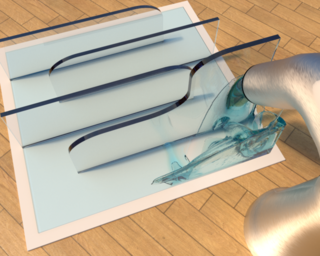
\includegraphics[width=.236\textwidth]{images/DD/snake_channel_060.png}
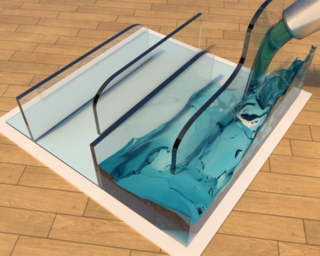
\includegraphics[width=.236\textwidth]{images/DD/snake_channel_180.png}
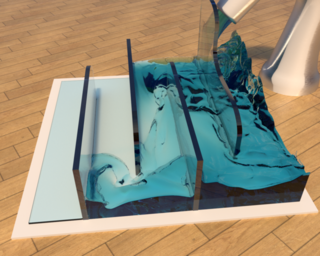
\includegraphics[width=.236\textwidth]{images/DD/snake_channel_320.png}
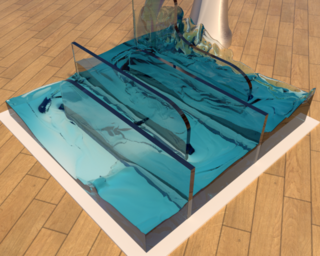
\includegraphics[width=.236\textwidth]{images/DD/snake_channel_540.png}
\end{center}
\caption{Free-surface simulation of water poured in a container with multiple interior walls causing the flow to meander around them. The frame shown in the right-most illustration corresponds to $114$ million active cells, in a $1024\times1024\times1024$ background grid.}
\label{fig:snake-channel}
\end{figure}

\textbf{Construction of adaptive operators} We construct the adaptively coarsened discretization of section \ref{sec:adaptive-approximation} based on a Galerkin
process. Let us consider the example of the finest level of the multigrid hierarchy. We define an interpolation operator $P^\ast_h$ that ``prolongates'' the adaptive
degrees of freedom $x^\ast$ into their trilinearly interpolated uniform counterparts $x=P^\ast_hx^\ast$ (this interpolation is conscious of any T-junctions). Thus,
the adaptive discretization of the Laplacian is simply computed as $A_h^\ast=(P^\ast_h)^TA_hP^\ast_h$. In fact, we never explicitly build the uniform matrix $A_h$,
but rewrite this equation as
$$
A_h^\ast=\sum_{a_{ij}\ne 0}a_{ij}\mathbf{p}_i\mathbf{p}_j^T
$$
where $a_{ij}=[A_h]_{ij}$, and $\mathbf{p}_k^T$ denotes the $k$-th row of $P^\ast_h$. This formulation allows us to construct the adaptive discretization directly
(by iterating over the uniform grid, and processing every spoke $a_{ij}$ of any stencil we encounter), without ever building the uniform matrix. Since our smoother
(Algorithm 2) never needs to use the \emph{uniform} subdomain discretization, we construct the adaptive discretizations of coarser levels of the hierarchy 
$A_h^\ast$, $A_{2h}^\ast$, $A_{4h}^\ast$, etc. by selective (Galerkin) coarsening of the immediately finer \emph{adaptive} discretization, rather than coarsening the
corresponding uniform discretization at that level into an octree.

\textbf{Avoiding nullspace issues} Global nullspace components (pockets of fluid with purely Neumann boundary conditions) are handled at the top-level PCG algorithm
via projection, as usual. In our smoother subroutine, we generally have the guarantee that the left-hand-side matrix $A_{\Gamma\Gamma}$ will be positive definite (it
is always symmetric), if the global matrix $A$ is definite too. However, it is possible for nullspace components to appear in the coarsened version of this matrix
$A_{\Gamma\Gamma}^{2h}$, $A_{\Gamma\Gamma}^{4h}$, as a result of the Galerkin procedure, in the vicinity of Neumann domain boundaries. To avoid this, we slightly
shift the eigenvalues of every coarsened discretization, say $A_{2h}^\ast$ by adding a minute multiple of the identity. The shifted matrix $A_{2h}^\ast+\epsilon I$
is practically spectrally equivalent to the original, and fully appropriate as a substitute in a multigrid hierarchy. Since we use direct solvers to invert
$A_{\Gamma\Gamma}$ in the smoother, conditioning is not an issue. Effectively, this eigenvalue shift will penalize solution components that lie in the nullspace to
be effectively equal to zero.

\textbf{Boosting accuracy} We use a high-order defect correction technique \cite{trottenberg:2001:multigrid} to allow our approximate inverse of a first-order
discretization to be used as a CG preconditioner for a higher order scheme. We structure our top-level PCG solver to implement matrix-vector multiply operations in
accordance with a second order accurate discretization of the Laplace operator \cite{Enright:2003:UTP}. Upon invocation of the preconditioner, however, we perform
the following steps: (i) We execute a few iterations of a Jacobi smoother, using the 2nd order operator, (ii) we then compute the residual, and multiply this with
our first-order preconditioner, and finally (iii) we again compute the residual $r$, write the error equation $Ae=-r$ using the second order operator, which we solve
using the same number of Jacobi iterations. We finally add the correction back to the result returned by the preconditioner. This operation, as described, preserves
the symmetry and definiteness of the preconditioner, and allows the first order method to be used as an effective preconditioner for the second-order problem (at the
comparably minimal expense of some additional smoothing effort near the high-order interface).

\textbf{Sparse grid storage}
 We used an ad-hoc sparse grid data structure to hold our grid data, for all
our examples which utilized highly irregular, sparsely populated grids.
 Our data structure partitions a virtual enclosing grid into rectangular blocks (of typical size $8^3$ voxels, in our examples), and stores them in a linearized array,
maintaining explicit pointers to the $26$ neighboring blocks to facilitate traversal during kernel invocation. This representation is reflected in both our CPU and GPU/Xeon Phi
implementations of all performance-sensitive kernels.

\begin{figure}[h]
\begin{center}
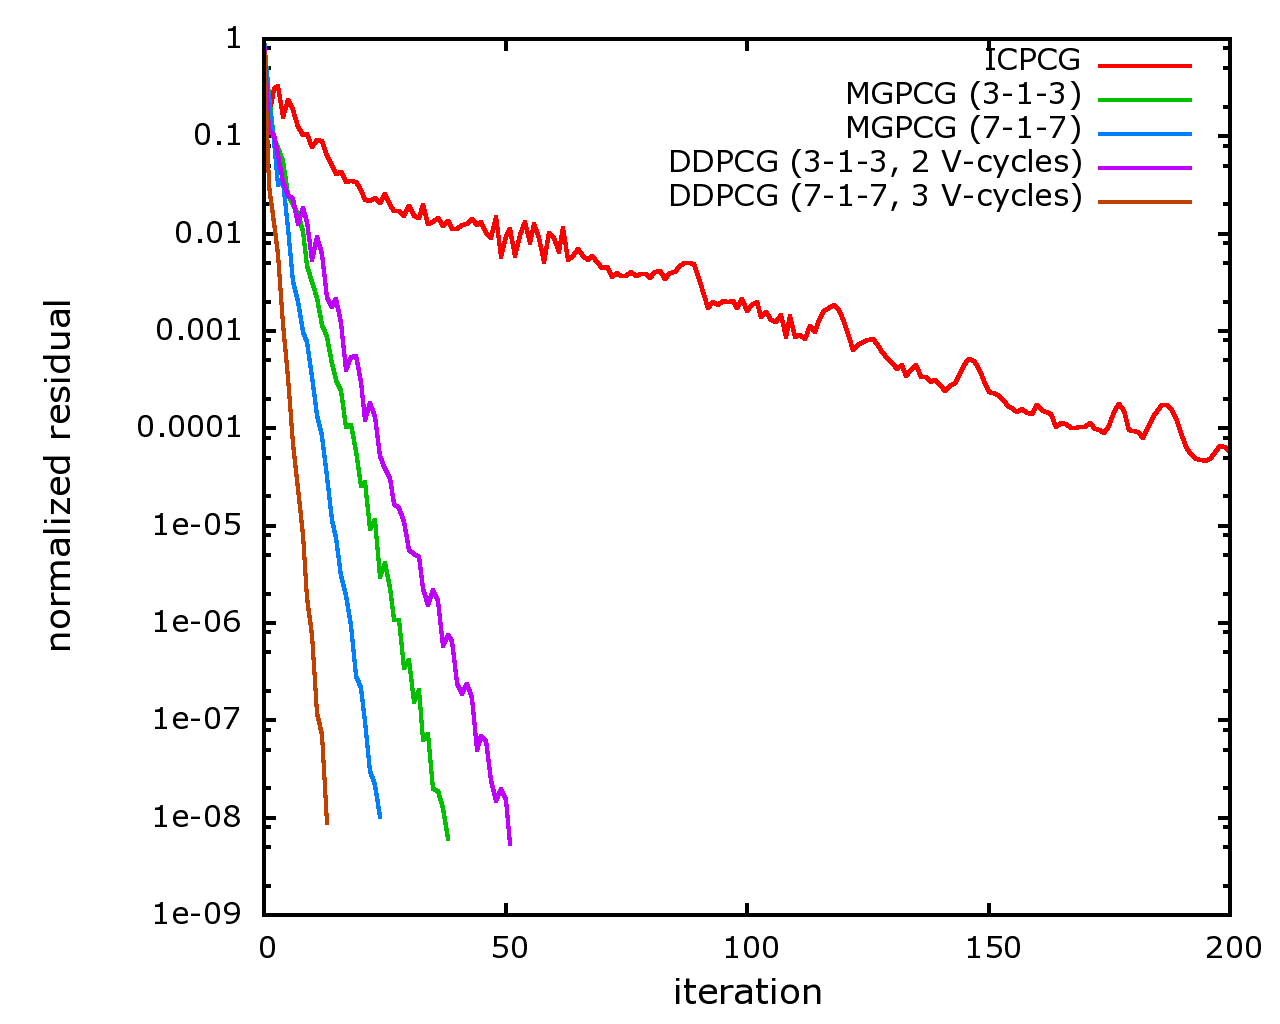
\includegraphics[width=0.48\columnwidth]{images/DD/convergence_plot.png}
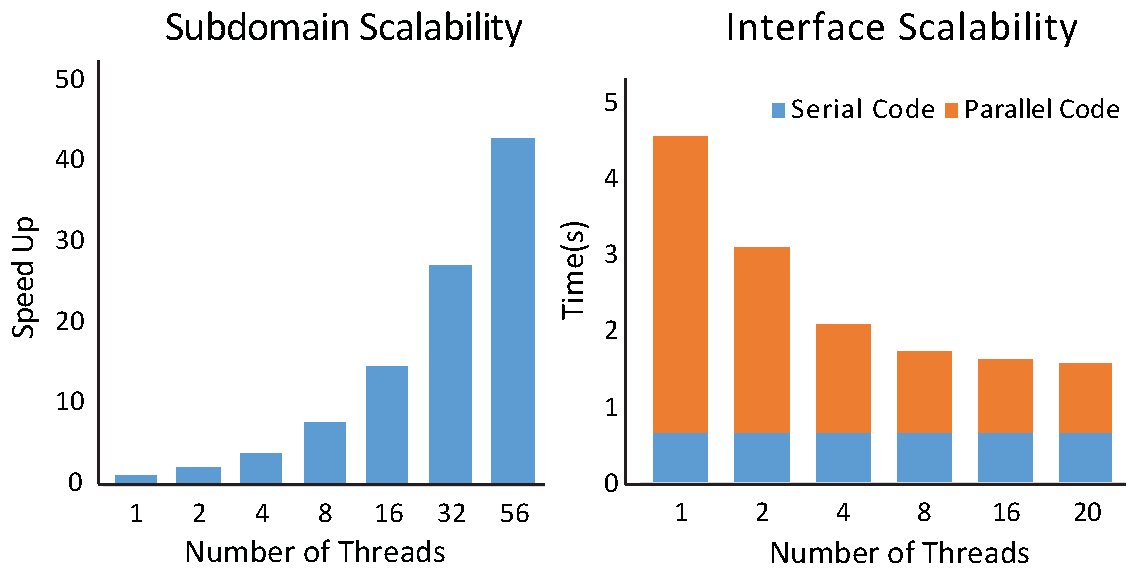
\includegraphics[width=0.48\columnwidth]{images/DD/scalability.pdf}
\end{center}
\caption{
\changed{(Top) convergence profiles for ICPCG, MCPCG and DDPCG (our method) from the water simulation of Figure \ref{fig:snake-channel}. The numbers ($B$-$I$-$B$) indicate
  multigrid smoothers that perform $B$ boundary sweeps, then $I$ interior sweeps, and $B$ more boundary sweeps at the end. V-Cycle counts in DDPCG reflect the number of cycles
  used in the approximate solution of each subdomain. (Bottom) Scaling of subdomain solvers (left; on Xeon Phi) and interface solver (right; on CPU) relative to the active cores/threads utilized.}
{ Convergence profiles for ICPCG, MGPCG (1 V-cycle, 3 boundary and 1 interior smoothing iteration), MGPCG (1 V-cycle, 7 boundary and 1 interior smoothing iteration), DDPCG (2
  V-cycles per subdomain, 3 boundary and 1 interior smoothing iteration), and DDPCG (3 V-cycles per subdomain, 7 boundary and 1 interior smoothing iteration).}
}
\label{fig:convergence-profiles}
\end{figure}


\section{Incompressible free surface flow}
\label{sec:free-surface}

We solve the incompressible Euler equations
$$
\vec{\boldsymbol{u}}_t+(\vec{\boldsymbol{u}}\cdot\nabla)\vec{\boldsymbol{u}} + \frac{\nabla p}{\rho} = \vec{\boldsymbol{f}}, \hspace{.4in}
\nabla\cdot\vec{\boldsymbol{u}} = 0
$$
using the splitting scheme as described in~\cite{Stam:1999:StableFluids}. Here,
$\vec{\boldsymbol{u}}=(u,v,w)$ is the velocity field vector, $\rho$ is the
fluid density, $p$ is the scalar pressure field, and
$\vec{\boldsymbol{f}}$ denotes external forces (such as gravity).
We discretize these equations on a MAC grid, where we first explicitly update
the advection terms
$$
\label{eqn:advection}
\frac{\vec{\boldsymbol{u}}^\star-\vec{\boldsymbol{u}}^n}{\Delta t}+(\vec{\boldsymbol{u}}\cdot\nabla)\vec{\boldsymbol{u}} = \vec{\boldsymbol{f}}
$$
using a semi-Lagrangian scheme~\cite{Selle:2008:MacCormack} and then solve for the
pressure via a Poisson equation
$$
\nabla\cdot\frac{\nabla p}{\rho}=\frac{\nabla\cdot\vec{\boldsymbol{u}}^\star}{\Delta t}
$$
in order to update the intermediate velocity as follows
$$
\frac{\vec{\boldsymbol{u}}^{n+1}-\vec{\boldsymbol{u}}^\star}{\Delta t}+\frac{\nabla p}{\rho}=0
$$
For tracking the free surface, we generally follow~\cite{Enright:2002:ARC} using the
level set advection of~\cite{Enright:2005:FAS}, the
reinitialization scheme of~\cite{Losasso:2005:SATLMIF}, velocity extrapolation method of~\cite{Adalsteinsson:1999:FCEVLS},
and a second order accurate pressure discretization of~\cite{Enright:2003:UTP}.

\begin{figure*}[t]
\begin{center}
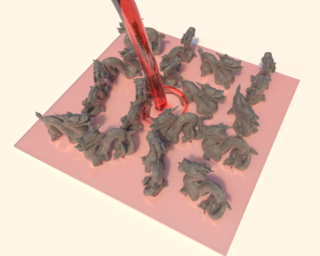
\includegraphics[width=.240\textwidth]{images/DD/dragons_028.png} 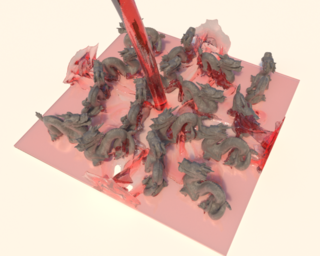
\includegraphics[width=.240\textwidth]{images/DD/dragons_050.png} 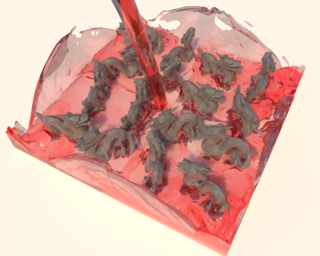
\includegraphics[width=.240\textwidth]{images/DD/dragons_115.png} 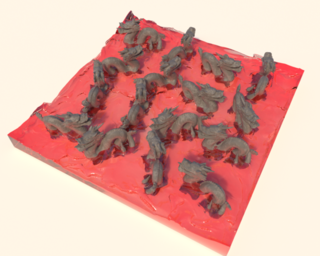
\includegraphics[width=.240\textwidth]{images/DD/dragons_220.png}
\end{center}
\caption{Water poured in a pool with multiple immersed objects. Second figure from the right shows $70$M  active cells, in a $1024^2\!\times\!512$ grid.}
\label{fig:free-surface-flow}
\end{figure*}

\section{Examples and performance benchmarks}
\label{sec:results}

We demonstrate the effectiveness of our preconditioner through several examples.
Figure~\ref{fig:DD-teaser} illustrates two smoke simulations with more than one billion of active degrees of freedom, each. 
Figure~\ref{fig:flasks} shows a network of interconnected vessels where smoke enters from the lower
left corner and exists from the upper right corner. Our solver is able to
capture the correct incompressible behavior in relatively few iterations with
four subdomains.  Figure~\ref{fig:free-surface-flow} shows an example where
water is poured in a pool with multiple immersed objects, creating complex
Neumann interfaces. Figure~\ref{fig:snake-channel} shows an example where water flows in
a channel with multiple interior walls, which cause the flow to meander around
them. Figure~\ref{fig:performance-results} provides a breakdown of individual kernels of our Schur Complement solver for all these examples, along with timings for alternative
solvers, detailed in the following section.\added{ We note that no vorticity confinement was used in our smoke examples. Finally, in the interest of efficiency we used as high of a
  CFL number as our examples could tolerate -- sometimes leading to minor loss of detail}.


\section{Discussion}
\label{sec:discussion}

\paragraph{Evaluation of convergence and scaling}

In our benchmarks, we compared the convergence behavior of our Schur-Complement Domain Decomposition preconditioned CG \emph{(``DDPCG'')} with a standard Incomplete Cholesky
preconditioner \emph{(``ICPCG'')} \cite{Foster:2001:PAO}, and a standard Multigrid-Preconditioned CG algorithm \emph{(``MGPCG'')} \cite{mcadams2010parallel}. For
the multigrid option, specifically, we note that although we did not experiment with improved CPU-based versions of MGPCG that take extra steps to better capture the topology of
the domain on coarser levels of the multigrid hierarchy \cite{Westermann:2014:LiquidAdaptiveHexahedral}, we invested a significant effort to optimize the stock MGPCG to the
absolute best of our capacity, both on the CPU as well as on the accelerator cards  -- this was a natural
step to take, as the multigrid kernels used in MGPCG are re-used in the subdomain solver of our own DDPCG method. We produced two, heavily optimized MGPCG implementations:
One designed to run exclusively on the CPU, and one designed to run \emph{homogeneously} 
on just a single GPU, for problems that are small enough to fit entirely in GPU memory. There is only one algorithmic difference between the two implementations: The pure-CPU MGPCG
was set up to solve the coarsest level of the multigrid hierarchy using ICPCG -- this was done to improve the convergence behavior at the bottom of the multigrid cycle, which
was crucial in obtaining acceptable performance at our examples with more than a billion degrees of freedom (without requiring an extremely deep, and occasionally inaccurate
V-cycle). The GPU-native implementation of MGPCG used a large number of smoother applications at the bottom of the V-cycle (which was effective for its smaller problem size), to
avoid using Incomplete Cholesky on the GPU. We benchmarked the pure-CPU MGPCG solver on the faster (dual socket) of our two test platforms.

In all our examples, the ICPCG solver exhibited dramatically slower convergence performance than both MGPCG, and our proposed DDPCG method, often needing more than an order of
magnitude of iterations higher than DDPCG to reach comparable performance. We were unable to use ICPCG for our largest of examples with billions of cells, as the footprint of the
explicitly constructed matrices would cause it to run out of memory. For our smallest examples, even each iteration of our heterogeneous DDPCG actually required less time than one
CPU-based ICPCG iteration. As a consequence, we did not find ICPCG to be a competitive alternative. 

On the other hand, the convergence behavior of MGPCG remained competitive in several of our smaller-size examples. We should point out that the behavior of DDPCG is tunable;
investing more V-cycles in the independent subdomain solves, or additional multigrid iterations in the interface solve can boost its convergence efficiency. We found MGPCG to be
most competitive with our DDPCG technique in the context of our smaller examples, especially the free-surface water simulations. This is attributed to the prominence of Dirichlet
boundary conditions in those scenarios, which dramatically improves the efficacy of smoothing boundary regions, which is essential for multigrid to behave favorably as a
preconditioner \cite{mcadams2010parallel}. On average, across the various frames of the water simulations (Figures
\ref{fig:snake-channel},\ref{fig:free-surface-flow}) MGPCG would converge in no more than $1.5$x-$3$x the number of iterations required by our tuned DDPCG, while in the smoke
simulation of Figure \ref{fig:flasks}, MGPCG required approximately $2$x-$2.5$x more iterations than DDPCG. In terms of run time, however, the findings paint a quite different
picture. The smaller two of our examples (Figures \ref{fig:flasks}, \ref{fig:free-surface-flow}) were compact enough to fit on just a single GPU card, where a single iteration of MGPCG
was between $5$x-$8$x times faster than a DDPCG iteration. Thus, in spite of the moderately slower convergence of MGPCG, its faster per-iteration cost on the homogeneous,
single-GPU implementation makes it preferable to DDPCG by a factor of $3$x-$5$x. Incidentally, the geometry of the smoke example in Figure \ref{fig:flasks} led to another
interesting observation: Although the narrow cylindrical connectors between the glass spheres allowed for a small interface between subdomains used in our solver (and a
reduction in CPU computation cost), the same geometry traits increased the approximation error induced by our adaptive coarsening of the subdomain interiors, increasing the
required iterations for PCG convergence.

The situation is dramatically different for our larger simulation examples, which cannot be solved with MGPCG on a single accelerator card. For those examples, the only practical
alternative was to run MGPCG homogeneously on the CPU. In this context, we observed that each iteration of our DDPCG method was within $20\%$ of the cost of a CPU-only MGPCG
iteration. However, for the large-scale examples, dominated by Neumann boundary conditions, we observed MGPCG requiring up to $5$x more iterations for convergence, leading to a
$3.5$x-$4.5$x performance benefit of DDPCG versus the CPU-only MGPCG. We conclude that for small problem sizes, in the order of $100$M degrees of freedom or less, a
\emph{homogeneous GPU} implementation of MGPCG is the preferred solver, provided that the problem can fully fit in GPU memory. For problem sizes that do not fit completely in GPU
memory, DDPCG appears to be consistently superior to CPU-based MGPCG, with the performance gap becoming larger as the resolution increases.

\begin{figure}[t!]
\begin{center}
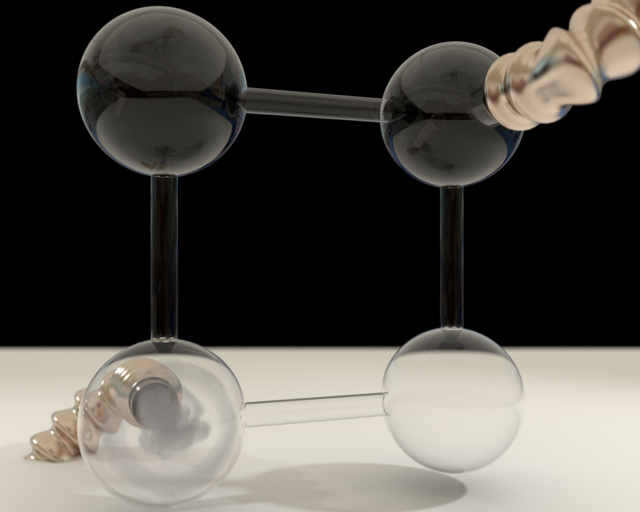
\includegraphics[width=.24\columnwidth]{images/DD/flasks_050.png} 
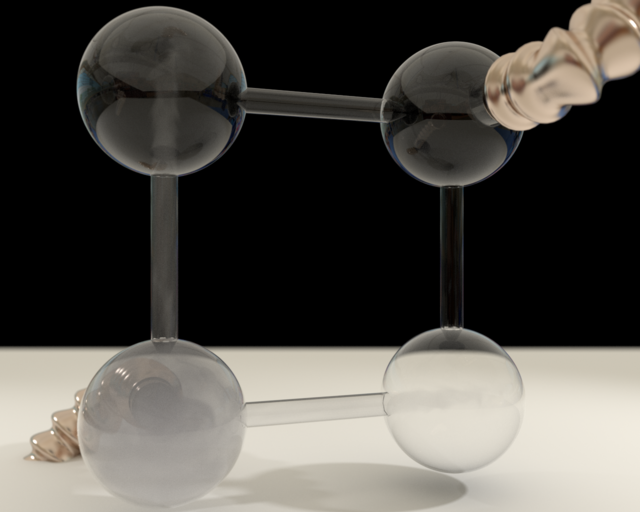
\includegraphics[width=.24\columnwidth]{images/DD/flasks_200.png} 
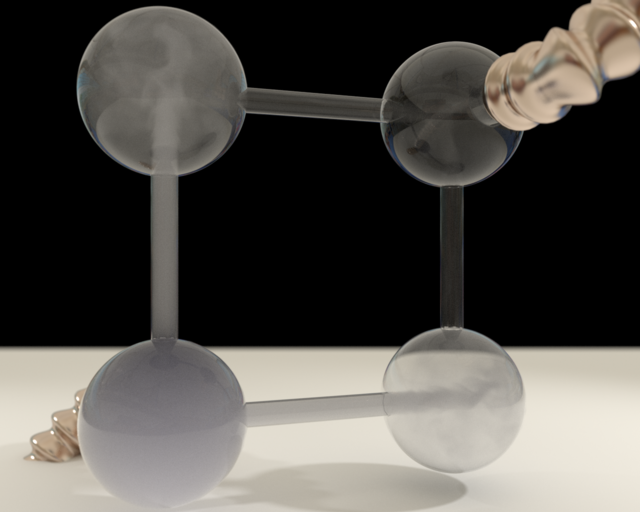
\includegraphics[width=.24\columnwidth]{images/DD/flasks_500.png} 
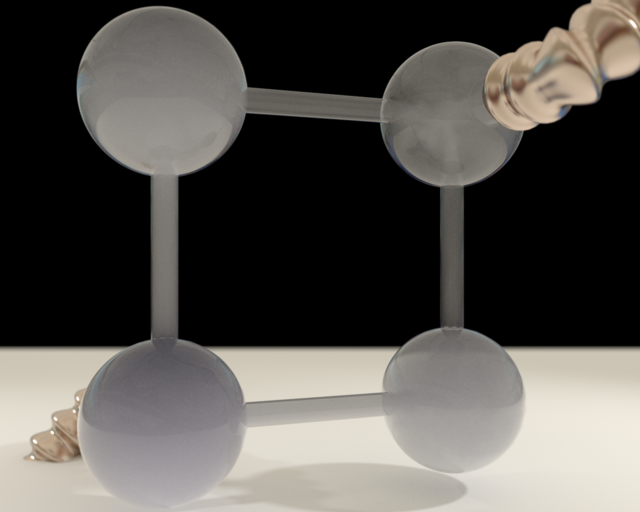
\includegraphics[width=.24\columnwidth]{images/DD/flasks_800.png} 
\end{center}
\caption{Smoke flow in a network of interconnected vessels simulated using a $1024^2 \times512$ background grid and $42$ million active cells. The computational domain was divided into four subdomains. The proper flux is observed both in the inlet and the outlet of the flow.}
\label{fig:flasks}
\end{figure}

\paragraph{Limitations and future work}

The most fundamental limitation of our proposed method is that, in order for its scaling benefits to take effect, it needs to be applied to a problem of adequately
large size. In designing our (GPU-hosted) multigrid cycle for the
solution of the subdomain problems, we made a conscious choice to keep the design of this solver as simple as possible, approximating the domain at voxel-accuracy at
every level, and not enacting any remedies for topological inconsistencies, such as regions merging or small Neumann gaps disappearing after coarsening. This was
done in the interest of simplicity, to facilitate low-level optimizations of the solver components. It is quite likely that topology-conscious coarsening schemes
\cite{Westermann:2014:LiquidAdaptiveHexahedral} could further improve the convergence properties of this component, and the balance between enacting such
improvements and retaining opportunities for aggressive optimization certainly merits investigation. Finally, one should not discount the software engineering
challenges that are still associated with developing numerical software that is as inherently heterogeneous as our solver. The established programming
paradigms that are available for \emph{homogeneous} thread-based parallel development (e.g. OpenMP) are arguably much more accessible to the non-expert
developer. Given the precedent of CUDA, and the growing presence of heterogeneity in modern systems, we hope that programming abstractions for these platforms
will continue to evolve. 

The scope of our work was specifically restricted to the design and optimization of the pressure Poisson solver on a heterogeneous computer. We also specifically targeted fluid
simulation on \emph{uniform} grids in the development of our solver. Although extending the concepts of our solver to an adaptive discretization is certainly possible from an
algebraic perspective, we feel that a careful investigation is warranted to make sure that 
the complexity of work that needs to happen on the interface region remains comparatively lower. This aspect, as well as practices for efficient dynamic partitioning
of temporally changing adaptive grids would be an exciting topic for continued investigation. 

A very interesting venue for future work might focus on extending our technique to deeper hierarchies of heterogeneous platforms, using for example clusters of
network-interconnected GPU-accelerated nodes. The same way that we used a multigrid cycle to approximate a subdomain solver, one could envision using our entire
preconditioner as the approximate solver for a subdomain assigned to each cluster node, which is internally subdivided to use GPU accelerations as we currently
do. Although bandwidths of network interconnects would be even slower than that of PCIe, due to economy of scale the relevant asymptotics (relative size of
interfaces vs. entire grid) could remain favorable. Finally, emerging GPU architectures and technologies (stacked memory, integration of CPU and GPU) might
facilitate programming in a homogeneous model (using capabilities such as unified memory spaces), but non-homogeneity in memory bandwidth is almost certain to
persist in some form (cores having significantly higher bandwidth to their ``local'' region of memory). We feel that the adaptation of solver concepts to such
architectural traits is an exciting research thread.

\begin{figure*}[t]
\begin{center}
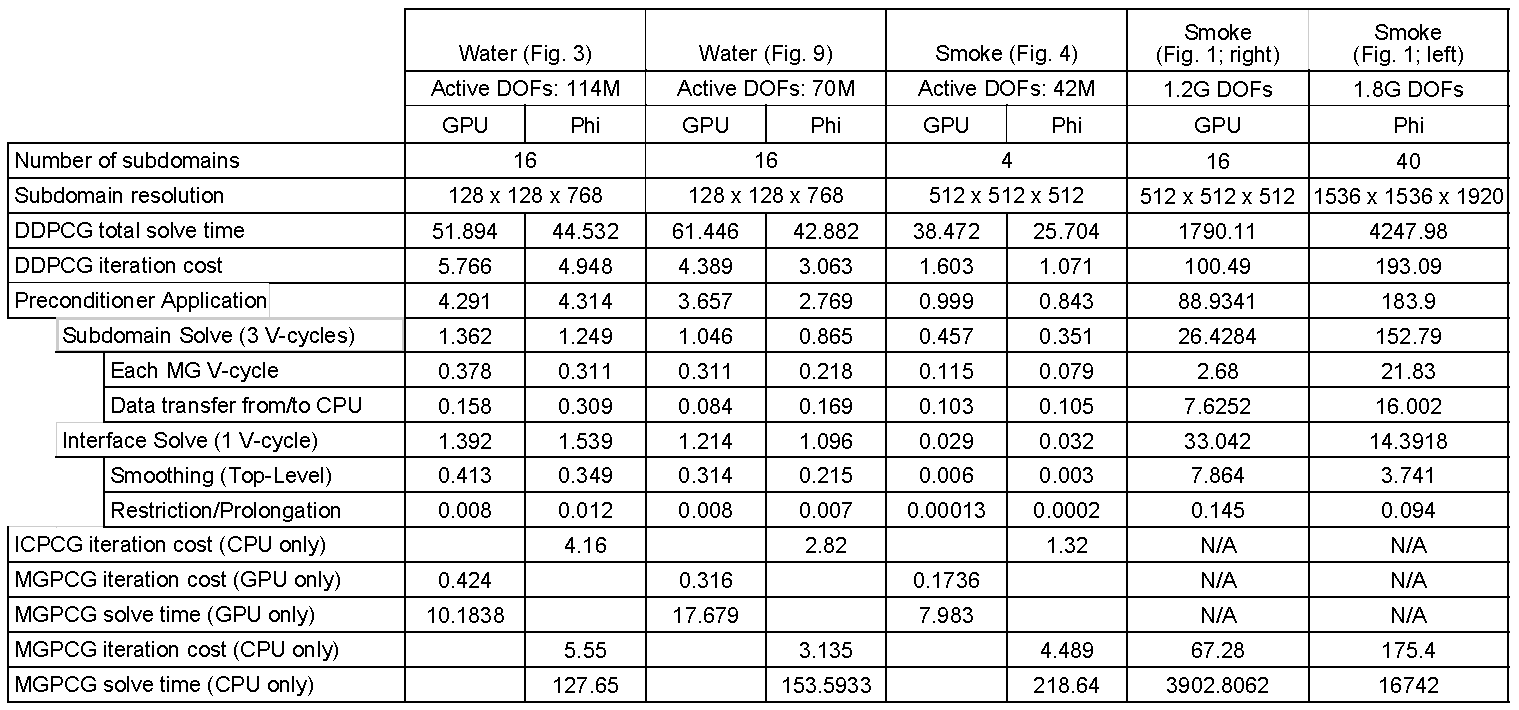
\includegraphics[width=.94\textwidth]{images/DD/performance_results.pdf}
\end{center}
\caption{Timing information for four examples. \textbf{All run times cited are in seconds}. Our ``GPU'' platform is an Intel Xeon
E5-1650v3 CPU equipped with two NVidia GTX Titan X GPUs and 128GB RAM, while our ``Phi'' platform is an Intel Xeon E5-2650v3 CPU equipped with six Intel Xeon Phi 31S1P cards.
\added{The row labeled \textsf{Preconditioner Application} reflects the preconditioning cost for a single PCG iteration.}
}
\label{fig:performance-results}
\end{figure*}


\chapter{Narrow-Band Topology Optimization on a Sparsely Populated Grid} 
\label{Chapter:Elasticity}
In the context of designing efficient solver, topology optimization, as an application, creates very interesting challenges to the numerical solvers. It desires high resolution, for many interesting details only emerges in high resolution simulation. It generates sparse domain, as in many scenarios only a fraction($<5\%$) of domain is filled in the final solution. It also creates high contrast ($1:10^{-9}$) material distributions. 

In this chapter, I present a design of efficient linear elasticity solver that is tailored for high resolution and sparse domain. Regarding the high contrast material distribution, I will demonstrate how it impairs the multi-linear multigrid solver's convergence rate, which inspired a design of stencil-aware interpolation scheme that drastically improves convergence rate in those situations.
\section{Topology Optimization Overview}
\begin{wrapfigure}{R}{0.45\textwidth}
\centering
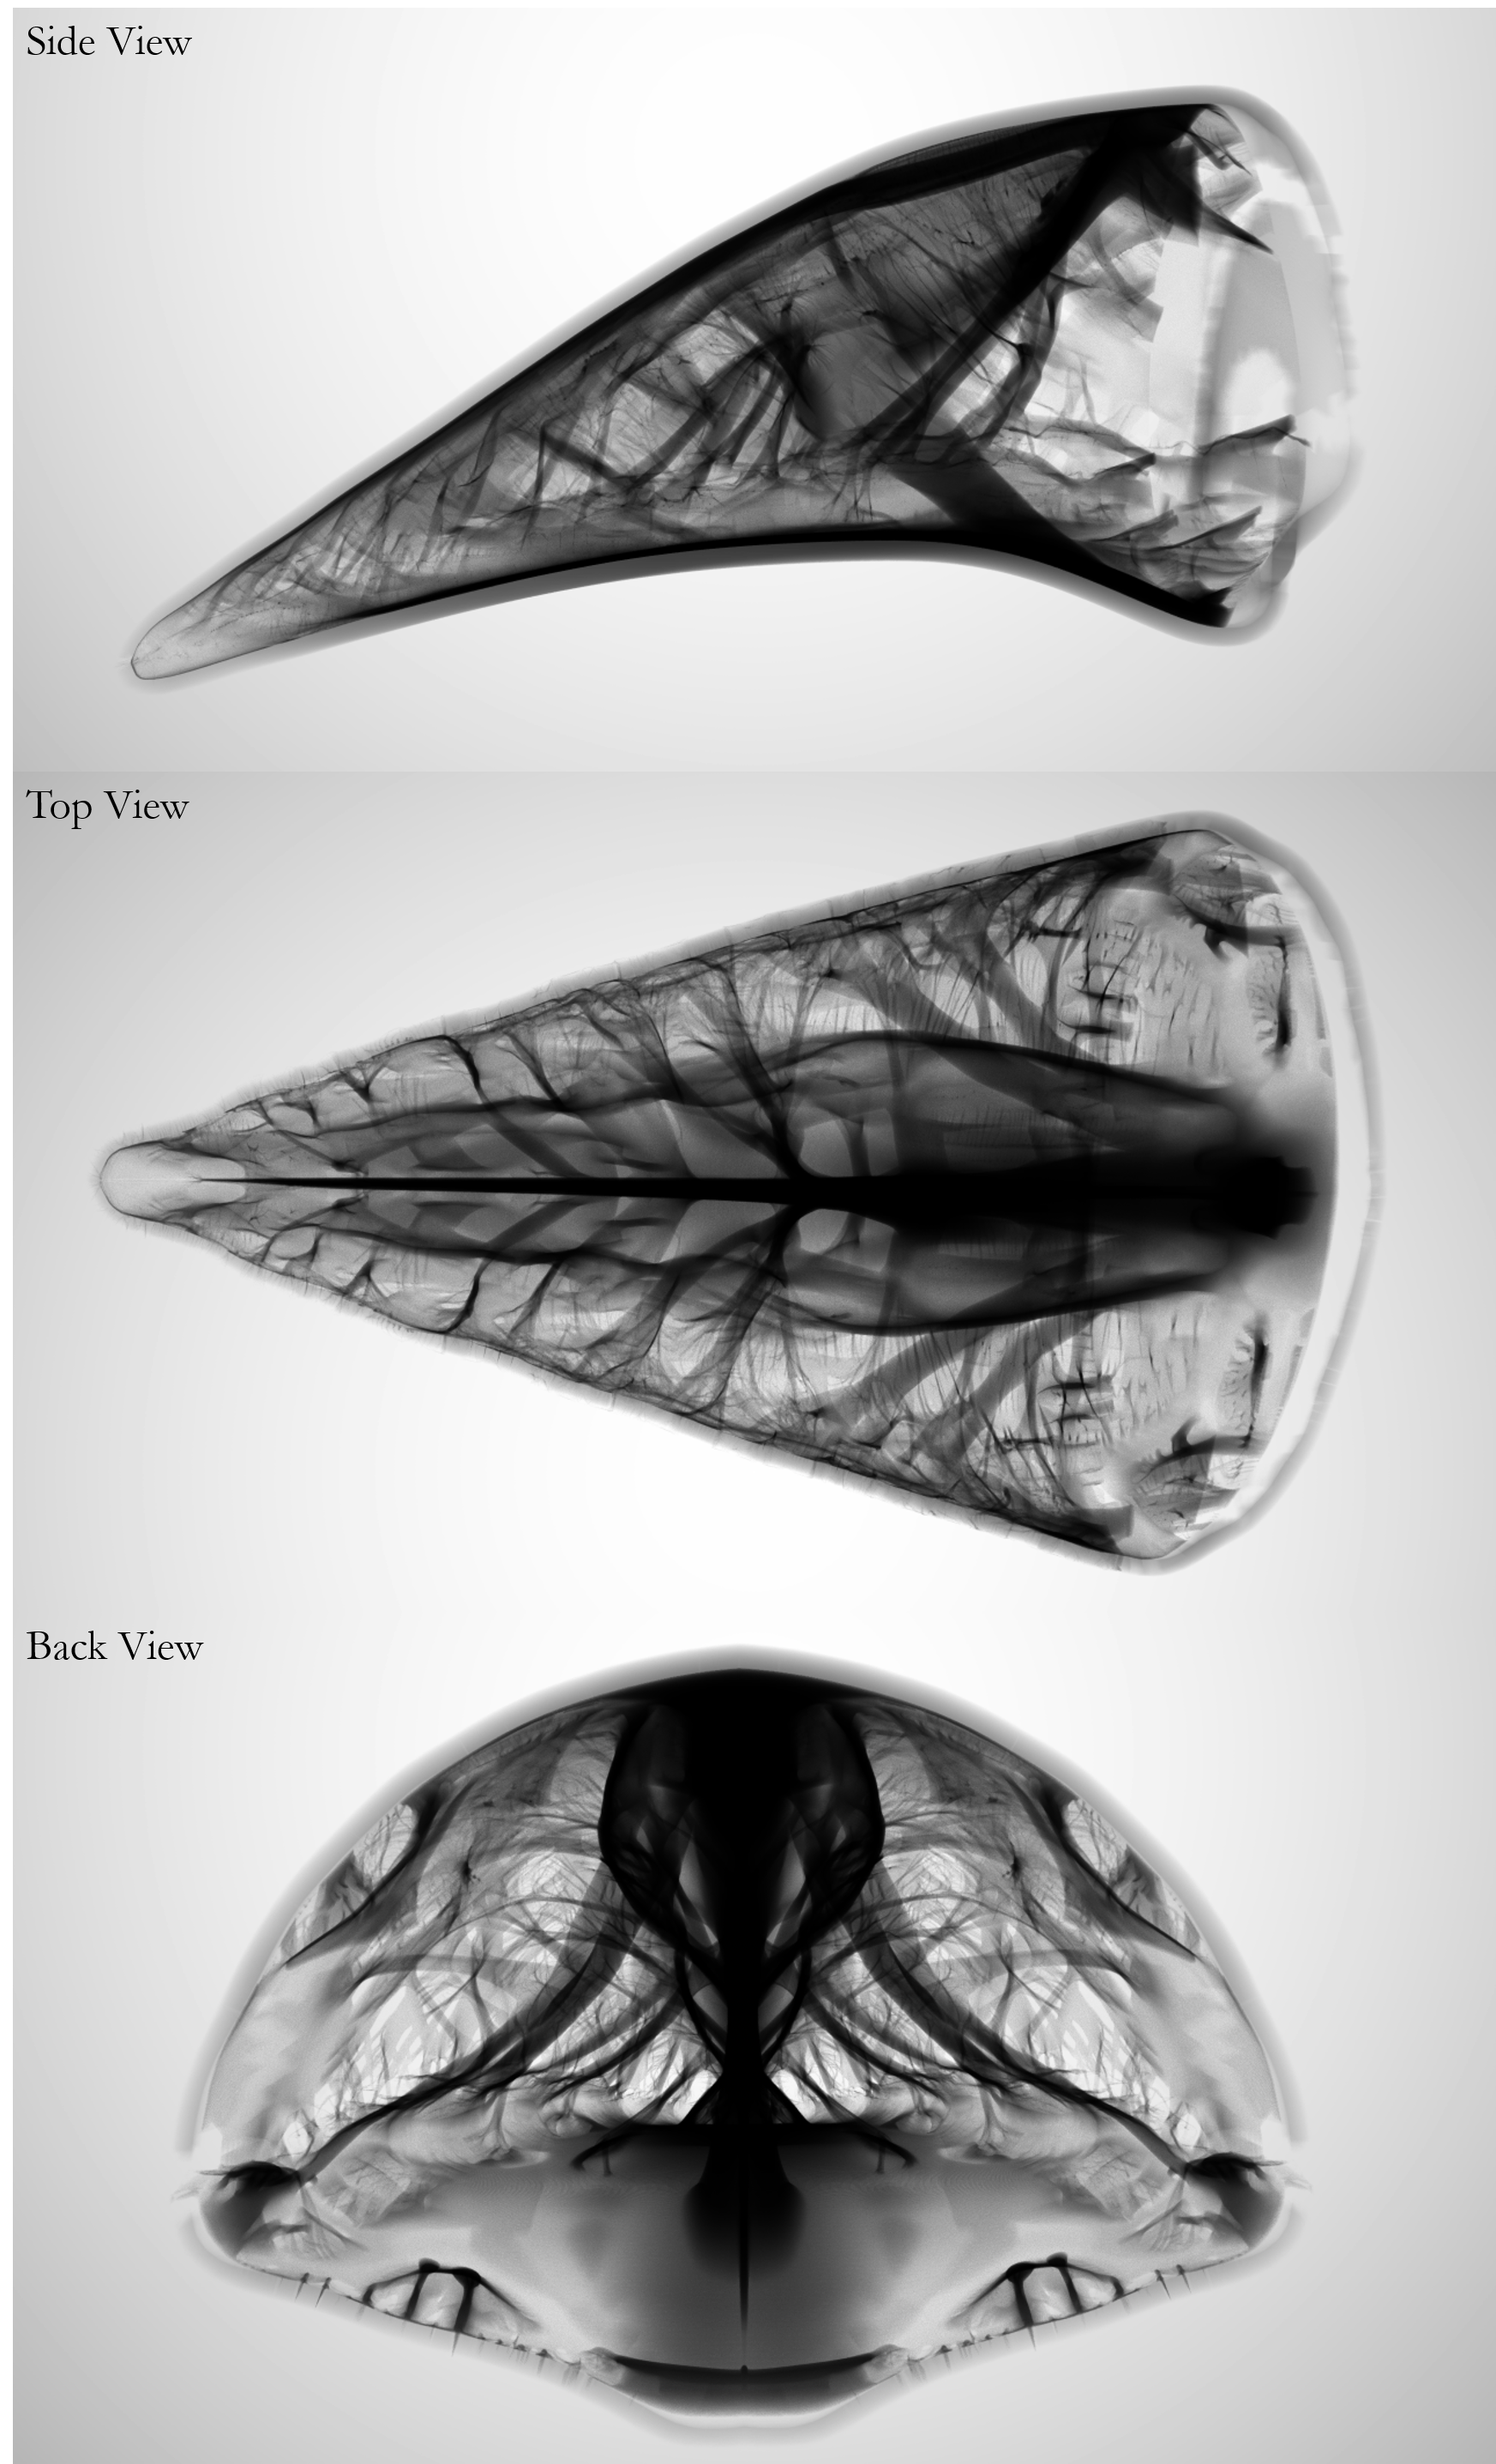
\includegraphics[width=0.42\textwidth]{images/TopOpt/beak_teaser}
\caption{The interior structures supporting the shell of a bird beak generated using our narrow-band topology optimization algorithm with $1,040,875,347$ (1.04 billion) active FEM voxels. The resolution of the background grid is $3000 \times 2400 \times 1600$. The three figures show the volumetric rendering of the same structure from different views.}
\label{fig:beak}
\end{wrapfigure}
Topology optimization aims to solve the problem of distributing materials in a given domain that minimizing the structural compliance or other objectives to given load(s).
It has demonstrated its efficacy in creating mechanical designs with complex structures and extreme properties in various engineering problems (see \cite{rozvany2009critical}, \cite{sigmund2013topology}, \cite{deaton2014survey} for surveys).
Starting from a volumetric domain that is uniformly filled with material, a standard topology optimization algorithm iteratively removes and redistributes material to develop a structure that minimizes a design objective (e.g., structural compliance), given the prescribed target volume and boundary conditions.  

However, due to the limitations of the previous computational frameworks, it is challenging to perform a standard topology optimization algorithm to emerge and evolve these thin and sparse features.
For example, to model the evolution of a thin sheet at the length scale of ten micrometers within a centimeter cube, it requires an FEM solver discretized on a $1000^3$ Cartesian grid. 
This grid resolution amounts to the order of magnitude of one billion active elements.

Recent advances in supercomputing provide some solutions that overcome this challenge.
For example, \cite{Aage2017GigavoxelCM} ran a parallel topology optimization program on a cluster with 8000 cores for days and obtained the structure of an airplane wing with the computational domain filled with 1.1 billion voxels.
A variety of novel, intricate, and multi-scale structures naturally emerge from the super-resolution computations.
This result is impressive, yet the limited accessibility and high cost of the supercomputing resources impede the use of such numerical approaches in a broader range of research and engineering applications. 
New computational tools, which are easy to access, efficient to run, and able to solve super-resolution systems, are needed in the scientific community.

\section{Main Contributions}
We propose a new computation framework that combines a sparse representation in conjunction with a highly optimized elastic multigrid solver for topology optimization, which delivers a significant leap in solving super-resolution problems from the prior state-of-the-art results.
Our framework has enabled the simulation of a sparsely populated computational domain on the level of billion active grid voxels on a single workstation. 
By examining the simulation results at such scale, we identify and analyze new challenges that have not been addressed, or even observed, in the previous research on elastic deformation simulation and topology optimization, such as poor asymptotic convergence of standard Galerkin-coarsened multigrid algorithm and the algorithmic limits of floating-point precision.

To address these scale-dependent challenges, we combined design practices and algorithmic interventions on data structures, numerical methods, and parallel solver implementations.
First, our framework is centered around a sparsely populated grid data structure, which allows the dynamic allocation of the degrees of freedom within a narrow band around the structure.  
This data structure combines the benefits of sparse storage, implicit topology representation, and the performance potential of high-throughput stream processing.
We have observed and demonstrated numerically that the elements with high structural sensitivities, which are essential for developing the structure towards its optimal topology, tend to bundle within a narrow band around the structure during evolution. 
In contrast, the vast bulk of void regions far from the structure contribute little to the total structural compliance, but they are the primary source of the computational cost in a dense discretization.
Therefore, the computation can be dramatically reduced by using a dynamically allocated sparse discretization, i.e the narrow-band representation.

In addition to the narrow-band representation, we developed a novel mixed-precision multigrid solver that is capable of solving FEM discretized linear elasticity in the order of billion elements on a single workstation.
By proposing an SPGrid-optimized matrix-free formulation for data storage and a novel mixed-precision computation, the solver can meet the memory storage and bandwidth demands of a multiprocessor workstation while maintaining high accuracy.
Also, our vectorized multigrid solver takes advantage of the AVX512 instruction set on the Intel Skylake-X/SP architecture in order to further enhance performance.

We summarize the main contributions of our work as follows:
\begin{itemize}
\item We demonstrate an ensemble of data structures, numerical schemes, and implementation best practices to perform topology optimization with the highest resolution (over one billion voxels) on a single shared-memory multiprocessor.
\item We propose a sparse, adaptive topology optimization framework where simulation of elastic deformation is restricted to a narrow band surrounding the high-density region.
\item We demonstrate the capacity of our framework to obtain a variety of complex thin and codimensional features, such as thin films and beams, that previous approaches might suppress.
\end{itemize}
\section{Method Overview}
Our sparse topology optimization framework consists of three key components: a sparse grid structure, a high-resolution multigrid FEM solver, and a narrow-band and unbounded structure optimizer. 
First, we briefly introduce the sparse paged structure (SPGrid) \cite{setaluri2014spgrid} as the base data structure to track the optimizing structures (Section \ref{sec:topopt_spgrid}). 
Next, we discuss our multigrid FEM solver for computing large-scale elastic systems on SPGrid in Section \ref{sec:topopt_multigrid}. 
Finally, in Section \ref{sec:topopt_result}, we provide method validations with respect to both the multigrid solver.

\section{Sparsely Populated Grid Structure}\label{sec:topopt_spgrid}
The Sparsely Populated Grid (SPGrid) data structure \cite{setaluri2014spgrid}, in comparison to other sparse  data structures, leverages the virtual memory system to allocate a very large virtual memory address span, corresponding to a sparsely populated background grid, while only materializing in physical memory the parts of this grid that are active. The allocation unit in SPGrid is a \emph{block}, a rectangular region of the Cartesian grid that is made contiguous in memory address space by virtue of a space-filling traversal scheme; The size of SPGrid blocks is chosen to be a multiple of a 4KB, i.e. the size of a physical memory page. SPGrid stores a number of data channels, which have similar sparsity pattern and corresponding indexing, in the same allocation block. Using the SPGrid data structure enables us to compute effectively on a sparsely populated domain with effective bandwidth comparable to a cache-optimized, dense uniform grid. In our multigrid FEM solver, we utilized the flexibility of SPGrid's block size, and chose a block size of $4\times 4\times 8$, tailored for vectorization as described in Section \ref{sec:topopt_multigrid}.
\section{Multigrid Solver}\label{sec:topopt_multigrid}
Our topology optimization framework utilizes a numerical solver for a lattice-based Finite Element Method (FEM) discretization of linear elasticity, with spatially varying material
parameters. In order to accommodate the large resolutions targeted by our method, we employ a solver based on the Multigrid-Preconditioned Conjugate Gradients (MGPCG)
algorithm. Algebraically, our methodology is similar to prior formulations of multigrid-preconditioned solvers [\cite{wu2016,dick2011real}], in employing a hexahedral discretization of
the linear elasticity operator, leveraging Galerkin coarsening to generate coarse level operators, and using a symmetric V-cycle as a preconditioner for Conjugate Gradients.
We deviate from standard practices as documented in prior work by way of design choices, data structures, and parallelization practices including: 
\begin{itemize}
\item A matrix-free implementation of the finest-level elasticity operator tailored for the SPGrid sparse storage structure.
\item A bandwidth-saving construction of the Galerkin coarsened operator at each level, which avoids streaming through explicitly-built matrices as input any only relies on
material properties at the finest level.
\item Storage of the explicitly formed coarse grid operators in a novel, SPGrid-specific banded sparse matrix format.
\item A modified eight-color Gauss-Seidel smoother designed to optimize memory bandwidth utilization and SIMD efficiency.
\item A mixed-precision implementation of MGPCG, which combines the accuracy of double-precision arithmetic with the storage saving
of single-precision representations.
\end{itemize}

\paragraph{Matrix-free design of finest level operator.} Due to the size of the simulation domains we target, economy in
memory footprint is essential to our approach. An explicit matrix storage at any level of the discretization would
necessitate 243 scalar coefficients per lattice node, consisting of 27 spokes of $3\times 3$ matrices. This number excludes
any compaction afforded by storing only the symmetric half of the operator, but also does not account for any additional
storage of matrix indices (e.g. in compressed sparse row format), or explicit topology storage of the computational
domain (e.g.  explicit hexahedral mesh). 

The SPGrid data structure provides the abstraction of a sparsely populated grid, without the need to explicitly
encode the connectivity of hexahedral simulation elements (e.g. as in an explicit mesh structure), as it is implied by
the background uniform grid topology. Although our computational domain is embedded in a large background regular grid
(up to the resolution of $3000\times 2400\times 1600$), its active cells in our simulation are only a sparse subset (up to 1.04 billion active cells, in our tests). The SPGrid structure allows us to directly store these active cells,
their material parameters as well as their nodal forces and displacements in a
sparsely populated grid. 

At the finest level, we
implemented a numerical kernel that computes the elastic forces resulting from the elasticity operator, for all nodes of a
given $4\times 4\times 8$ block of the SPGrid structure; this kernel is designed to be free of write-dependencies, hence
all blocks can be processed in parallel on different threads.

Consider a single grid cell with nodal displacements $\{\mathbf{u}_i\}_{i=1}^8$. We denote by $\{\mathbf{f}_i\}_{i=1}^8$
the nodal forces produced by the elastic response of the same cell, which can be expressed as 
$\mathbf{f}_i = \sum^8_{j = 1} \mathbf{K}_{ij} \cdot \mathbf{u}_j$. Each $\mathbf{K}_{ij}$ in this expression is a
$3\times 3$ matrix; we store these coefficients in a $8\times 8\times 3\times 3$ tensor $\mathcal{K}$, whose elements
are given by $\mathcal{K}_{ijvw}=[\mathbf{K}_{ij}]_{vw}$. This tensor is given as a linear combination of two canonical
tensors $\mathcal{K}^\mu$ and $\mathcal{K}^\lambda$\changed{}{ based on the Lam\'{e} coefficients}, corresponding to the stiffness matrices computed for
$(\mu,\lambda)=(1,0)$ and $(\mu,\lambda)=(0,1)$ respectively. \changed{It should be noted that $\mathcal{K}^\mu$ and
$\mathcal{K}^\lambda$ can either be computed by analytic integration of the linear elastic potential trilinear element}{They can be computed either by analytic integration of the linear elastic trilinear element},
or an eight-point Gauss quadrature rule. Ultimately, the elemental stiffness
tensor is expressed as $\mathcal{K}=\mu\mathcal{K}^\mu+\lambda\mathcal{K}^\lambda$. 
We use the notation $\mathcal{C}(i)$ for the set of eight cells incident to node $i$, while $\mathcal{V}(c)$ denotes the eight vertices at the corners of cell $c$. We can then express the total force on node $i$ as:
$$
\mathbf{f}_i = \sum_{c \in \mathcal{C}(i)} \sum_{j\in \mathcal{V}(c)} (\mu^{(c)} \cdot \mathbf{K}^\mu + \lambda^{(c)} \cdot \mathbf{K}^\lambda)_{i^{(c)}j^{(c)}} \cdot \mathbf{u}_j
$$
where $\mu^{(c)},\lambda^{(c)}$ are the parameters of cell $c$, and $1\leq i^{(c)},j^{(c)}\leq 8$ are the local indices of nodes $i,j$ as vertices of cell $c$. 
This operation can be trivially vectorized; let $\underline{\mathbf{f}}:=(f_{(p,q,r)},f_{(p,q,r+1)},\ldots,f_{(p,q,r+7)})$ be a SIMD vector of eight forces on nodes that are sequential along the $z$-axis, while $\underline{\mu}^{(c)}, \underline{\lambda}^{(c)}$ are the parameters of a cell neighbor for each of the eight sequential grid indices, and finally, $\underline{\mathbf{u}}_j$ the set of eight sequential nodal neighbors at a specific offset direction. The previous operation is then expressed as:
\begin{equation}
\underline{\mathbf{f}} = \sum_{c \in \mathcal{C}(i)} \sum_{j\in \mathcal{V}(c)} (\underline{\mu}^{(c)} \cdot \mathbf{K}^\mu + \underline{\lambda}^{(c)} \cdot \mathbf{K}^\lambda)_{i^{(c)}j^{(c)}} \cdot \underline{\mathbf{u}}_j .
\label{eqn:elasticity-stencil}
\end{equation}
We note that a SIMD line need not be structured strictly along a sequence of nodes aligned along the $z$-axis (or any other single axis); a rectangular arrangement, e.g. eight nodes straddling a $2\times 4$ rectangle along the $y$- and $z$-axes would work in exactly the same fashion. From a programming standpoint, equation (\ref{eqn:elasticity-stencil}) indicates that SIMD vectors of each Lam\'{e} parameter are scaled with a constant coefficient (a single multiply instruction, with embedded broadcast, in the AVX2 and AVX512 instruction sets), and multiply the respective neighboring displacements $\underline{\mathbf{u}}_j$ (a fused multiply-add operation) to compute a term contributing to
the nodal force $\underline{\mathbf{f}}$. With the increased number (32) of available registers in AVX512, we have verified that the entire stencil application can be executed with $2\times
24^2$ multiply and $2\times 24^2$ fused multiply-add instructions (FMA) without any register spilling, and enough distance between operation dependencies to allow the full throughput of \changed{2}{two}
FMA instructions per cycle in Skylake-X/SP\footnote{Intel Xeon Gold 6140 processor (18 cores at 2.30 GHz) with $192$ GB memory.} (approximately 1200 cycles for the stencil application on one 16-wide SIMD line).

\paragraph{Modifications to the SPGrid structure} In order to accommodate the SIMD-heavy stencil computations in our elasticity operator, we enacted two crucial modifications/enhancements of the baseline implementation \textsf{(http://www.cs.wisc.edu/\char`~sifakis/SPGrid.html)} of the SPGrid structure of \cite{setaluri2014spgrid}. The first of those, is a vectorized load routine, with a compile-time stencil offset, as in:
\begin{shaded}
\texttt{template <int di,int dj,int dk,class SPG\char`_array>}\\
\texttt{\char`_\char`_m512 VectorGet<di,dj,dk>(SPG\char`_Array a,int64\char`_t offset)}
\end{shaded}
where a 16-entry SIMD width in single-precision has been used, as an AVX512 example. The offset given as argument is presumed aligned at SIMD-width granularity, while a stencil offset 
$\texttt{(di,dj,dk)}$ is given as a compile-time argument. Using these semantics, grid data at a given stencil ``spoke'' (from an aligned baseline vector address) can be loaded for an entire SIMD line, as illustrated in Figure\ref{fig:simd_get}.
\begin{figure}[h] 
\center
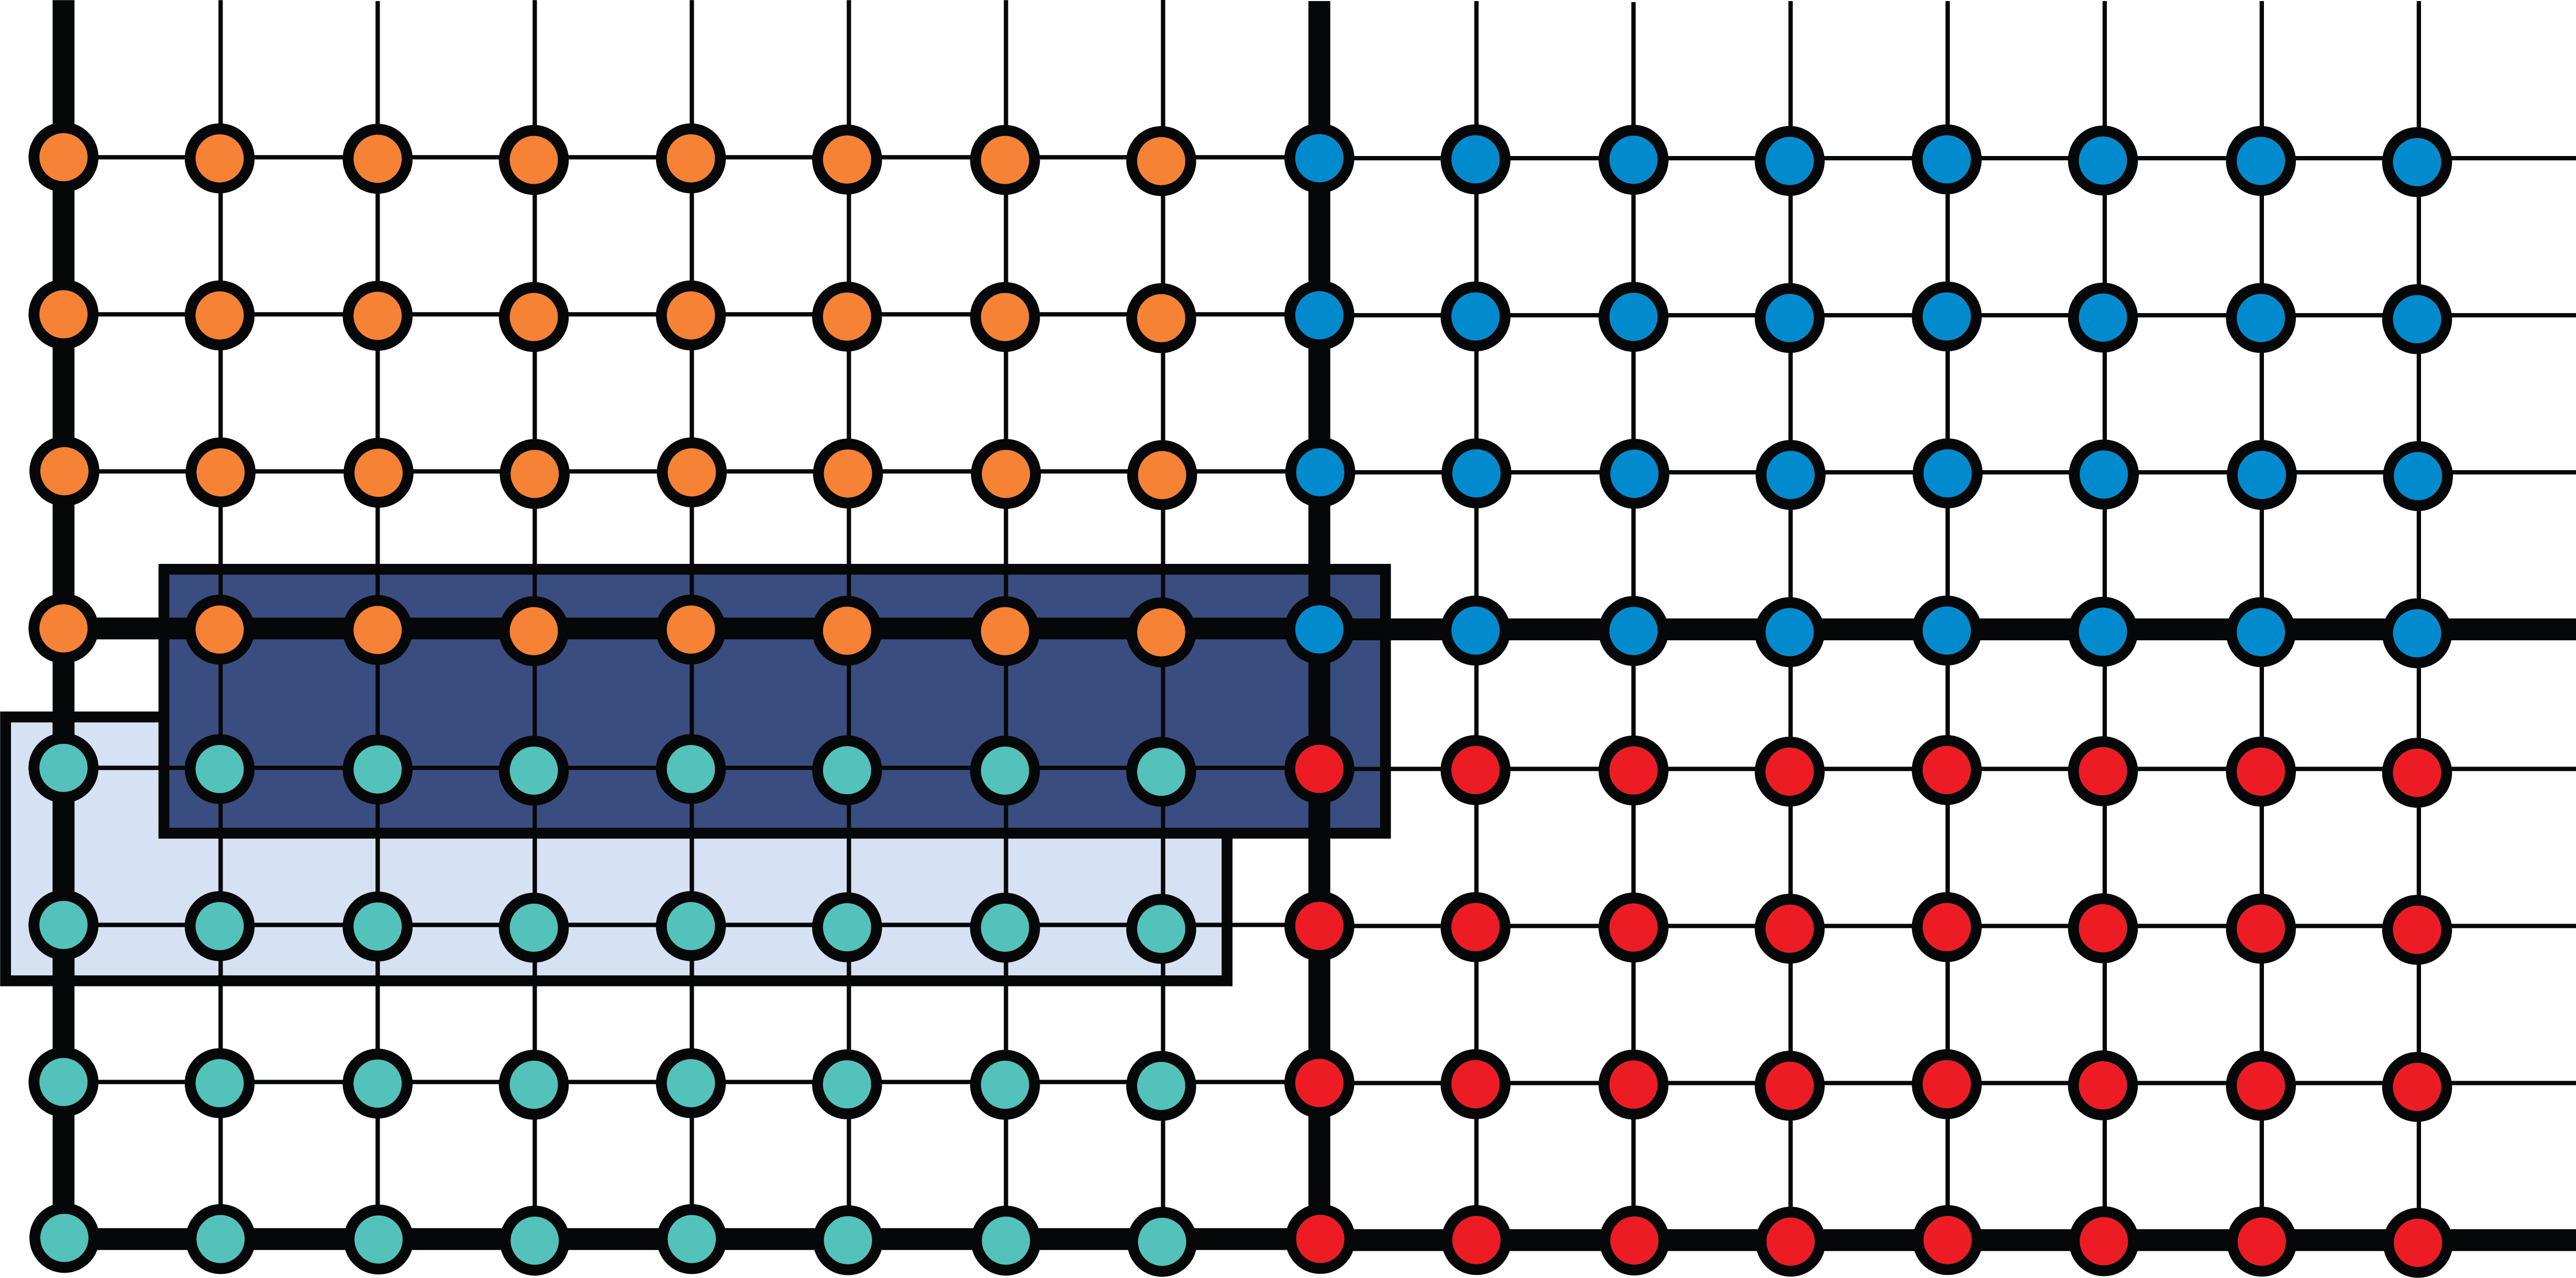
\includegraphics[width=.5\textwidth]{images/TopOpt/SIMD_Get}
\caption{The $\texttt{offset}$ passed to $\texttt{VectorGet}$ points to an sequence of SPGrid entries with SIMD-width alignment (light blue box). Using a stencil offset, e.g., shifts the region to be loaded by $\texttt{VectorGet}$, as shown in the dark blue box. The data of this shifted box may originate in several distinct SPGrid blocks (indicated by different node colors).}
\label{fig:simd_get}
\end{figure}
\noindent Even though the stencil shift might cause data to originate from different SPGrid blocks, the fact that such shift is known at compile time allows significant optimizations that avoid expensive gather operations and minimize address translations. 

The second SPGrid modification was the relaxation of the design restriction in \cite{setaluri2014spgrid} that each SPGrid block be sized to exactly 4KB (the size of a virtual memory page). Our solver used a total of $128$ bytes for all variables stored at each grid index, leaving the block size to just $2\times 4\times 4$ when a 4KB block size is used. We found it more effective to be able to use a larger block size, namely $4\times 4\times 8$ in order to (a) minimize the number of SIMD stencil accesses that straddle multiple blocks, and simplify implementation of $\texttt{VectorGet}$, and (b) allow an adequate number of nodes to be present per-block, to ensure that even after eight-coloring (as required by our smoother, described later in this section), the nodes on each color are a multiple of the SIMD width, even on AVX512 systems. We include source code for both proposed SPGrid modifications, as a supplement to our paper. As an indication of performance, we have achieved an effective bandwidth of $17.45$ GB/s for our multiply kernel.


\paragraph{Efficient Galerkin Coarsening.} In the construction of the multigrid hierarchy, we used the Galerkin coarsening method, computing the coarse grid operator as 
$\mathbf{K}^{c} = \mathbf{P}^T \cdot \mathbf{K}^{f} \cdot \mathbf{P}$, where $\mathbf{P}$ is the prolongation matrix and $\mathbf{K}^{f}$ the fine grid operator. At all but the two finest
levels, we can afford to store the coarsened operator explicitly, as the reduced dimensionality of the coarse grid allows us to do so at one-eighth of the memory footprint that such
matrix would have occupied at the finer level. Our construction of $\mathbf{K}^{c}$ is tailored around the following implementation objectives:
\begin{itemize}
\item Neither $\mathbf{K}^{f}$ or $\mathbf{P}$ are presumed available in matrix form.
\item The rows of $\mathbf{K}^{c}$ should be computed independently, to avoid write hazards.
$^\dagger$\item We seek the flexibility to compute $\mathbf{K}^{c}$ at \emph{any} coarse level directly from the material parameters at the finest level, without depending on operators
  at intermediate levels.
\end{itemize}

\begin{wrapfigure}{r}{.35\textwidth}
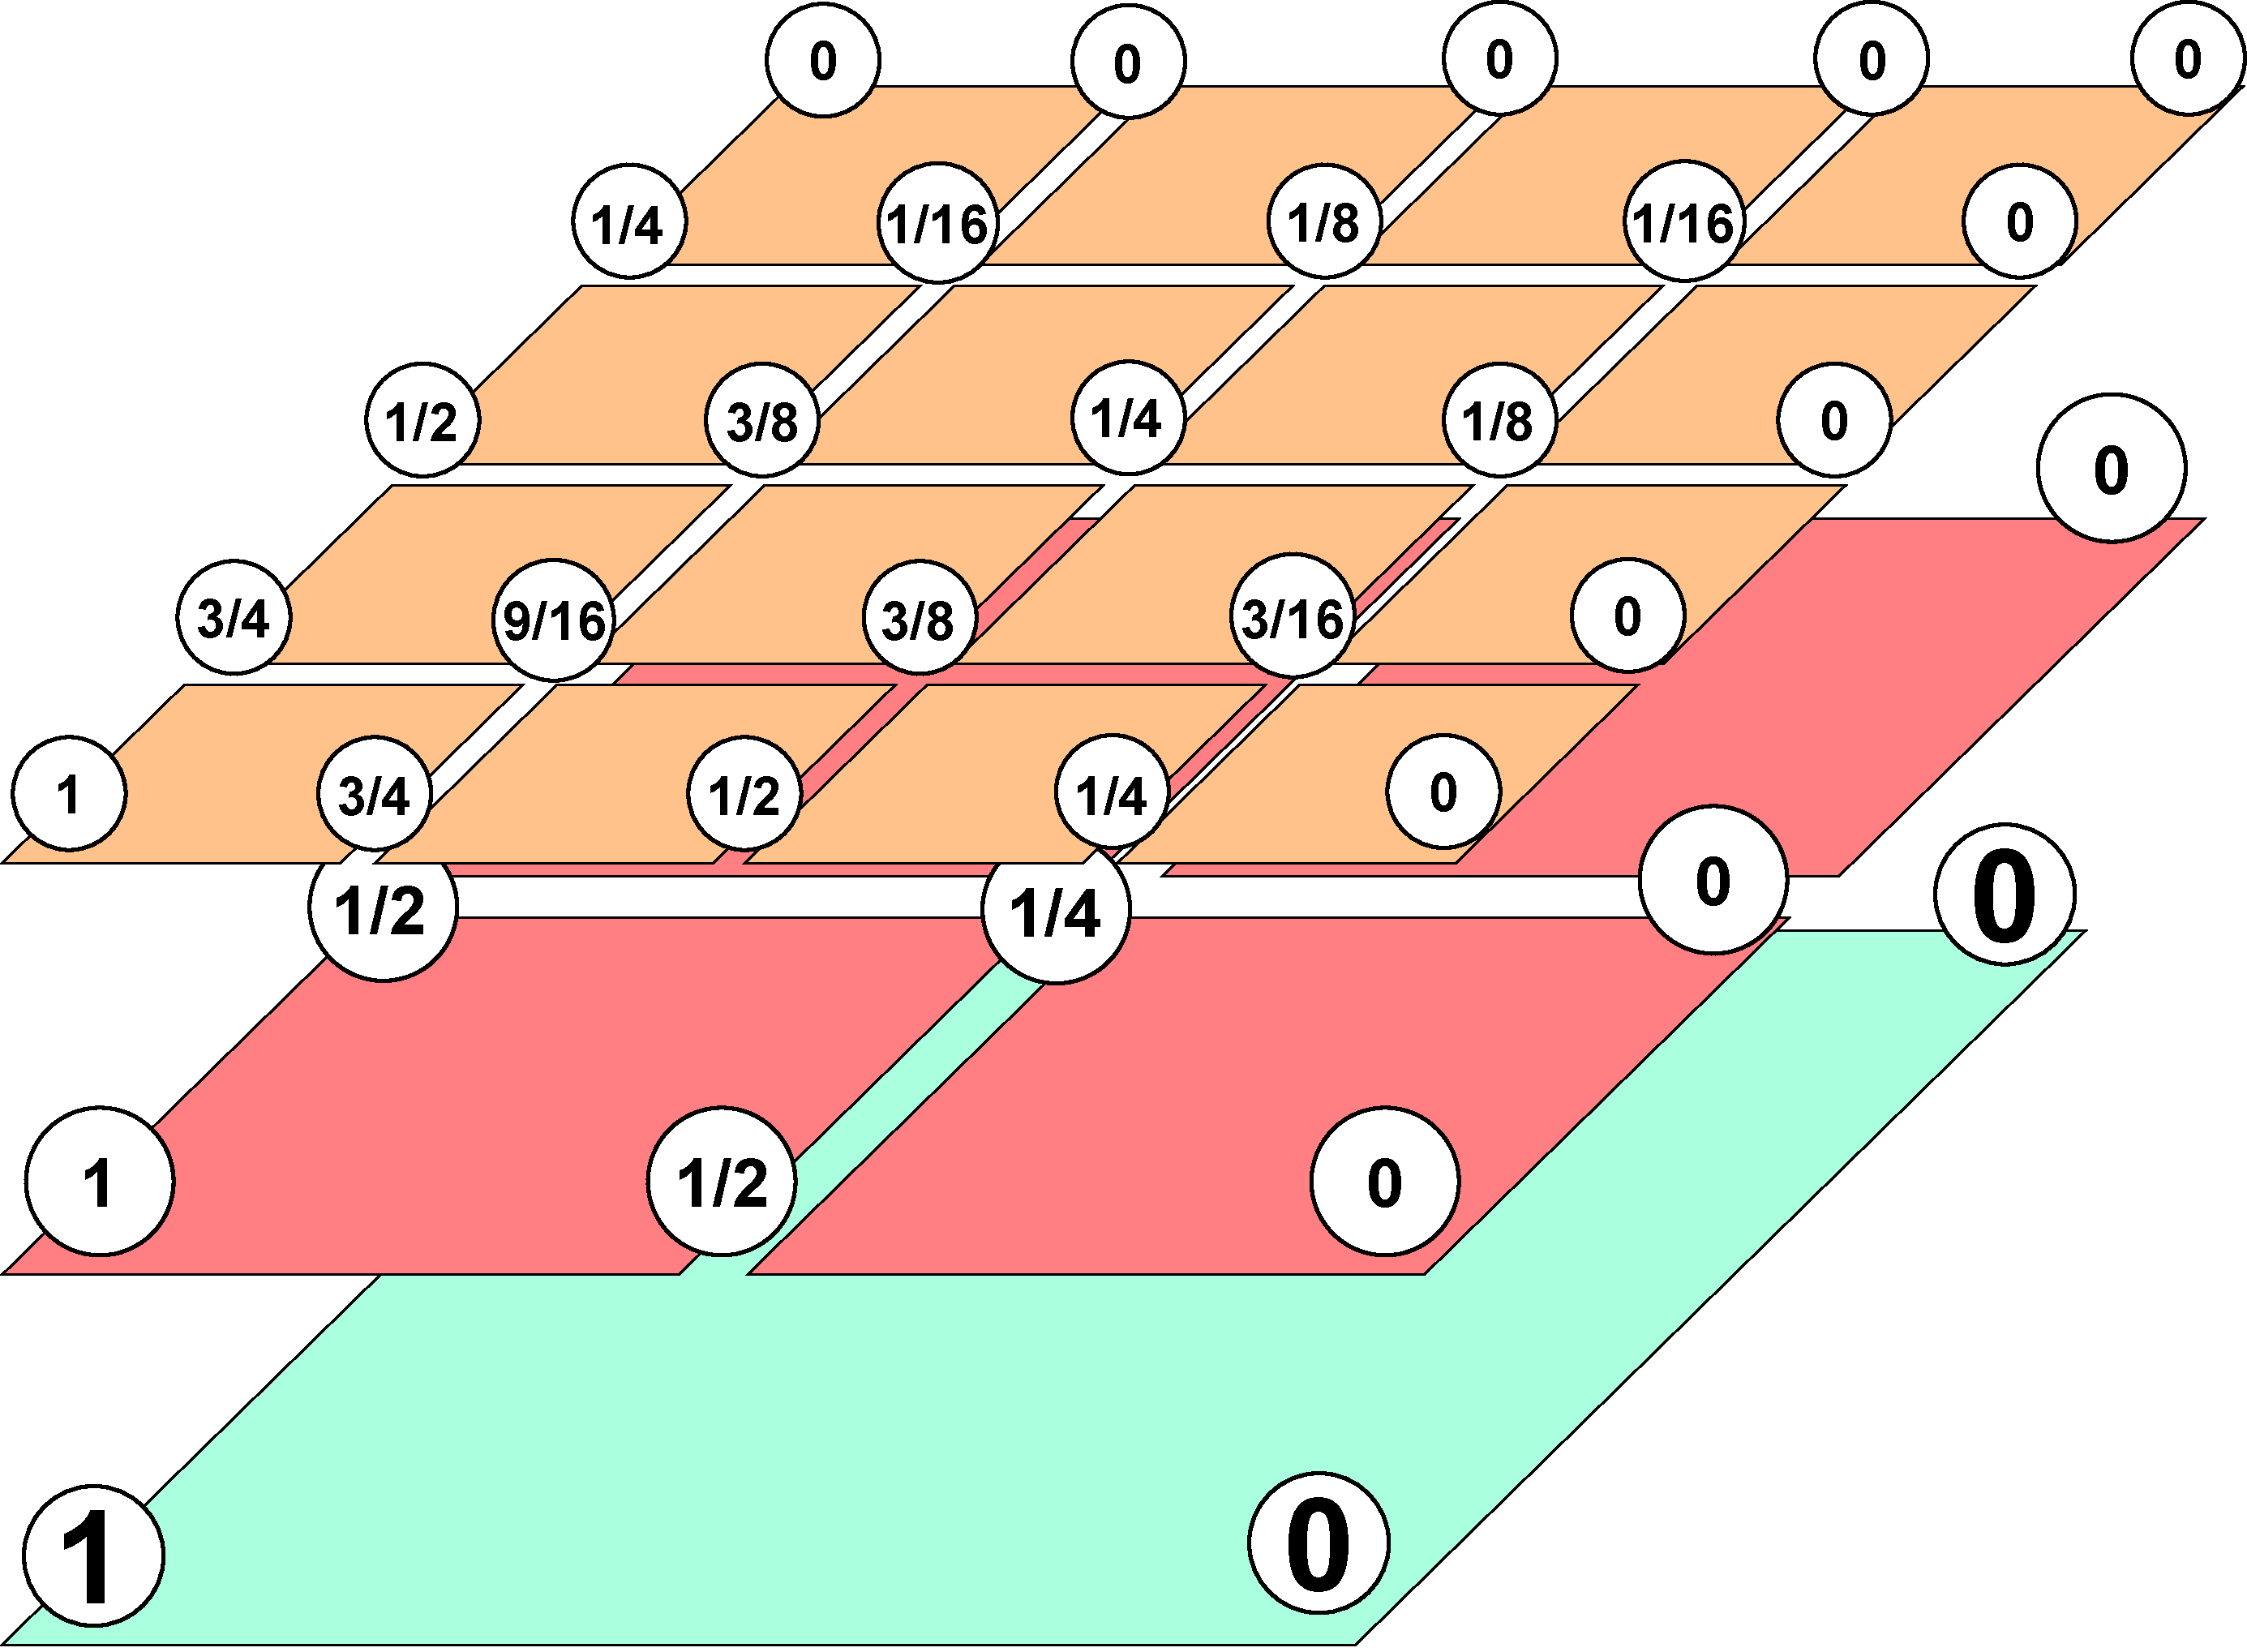
\includegraphics[width=.3\textwidth]{images/TopOpt/prolongation_v2}
\caption{Two successive prolongation operations on a Kronecker delta function during Galerkin coarsening of a coarse cell, illustrated in 2D.}
\label{fig:prolongation}
\end{wrapfigure}

Let us consider the specific example of constructing the operator $\mathbf{K}^{4h}$ at two levels coarser from the finest grid:
\begin{equation}
\mathbf{K}^{4h}=\mathbf{P}_{4h\rightarrow 2h}^{T}\mathbf{P}_{2h\rightarrow h}^{T}\mathbf{K}^h\mathbf{P}_{2h\rightarrow h}\mathbf{P}_{4h\rightarrow 2h}
\label{eqn:galerkin}
\end{equation}
The coefficients of the $i$-th row of this matrix (or equivalently, the $i$-th column, due to symmetry) are given by the action $\mathbf{K}^{4h}\mathbf{e}_i$ of this operator on the
basis vector $\mathbf{e}_i$. Equation (\ref{eqn:galerkin}) suggests that this action can be computed by successively prolongating $\mathbf{e}_i$ to the finest level, applying the
fine-grid operator $\mathbf{K}^{h}$, and restricting the result back to the coarse grid. 
We perform this operation separately on each of the eight cells (at level $4h$) incident on node $i$,
as illustrated in Figure~\ref{fig:prolongation}. The input to this process is a discrete Kronecker delta, shown as the input coefficients to the coarsest level. 
We can use an eight-wide SIMD register to store all eight nodal values of this
coarse cell. We have implemented a routine $\textsf{ProlongateCell()}$ that interpolates this eight-value SIMD register into eight more eight-wide registers corresponding to the nodal values of
the child cells at the immediate finer level. This routine is called recursively to prolongate all the way to the finest level. At that point, a routine $\textsf{CellMultiply()}$ is used
to compute the force response of each individual fine cell to these prolongated nodal displacements (using the material properties at the finest level). 
A routine $\textsf{RestrictCell()}$ implements the adjoint of the prolongation operation by collecting force contributions from fine child cells to their coarser parent. Since these routines are
called recursively, all SIMD vectors are stack-allocated and can be effectively cached.
As an indicator of performance, the construction of the entire operator hierarchy in our 1.04\changed{B}{ billion-}voxel example (Figure \ref{fig:beak}) requires 113.9 seconds using AVX512 instructions, which is a very small fraction of the MGPCG cost at this resolution.


\paragraph{Sparse Matrix Storage} The storage of the Galerkin-coarsened matrix needs to be handled as to exploit sparsity, facilitate the application of the smoother routine,
and allow a direct solver (in our case, Intel MKL PARDISO) to be used for solving the problem at the coarsest level of the hierarchy. Given that the topology of the background is a regular
Cartesian lattice, we use a band-storage approach, where the 243 nonzero coefficients associated with the stencil each node (a $3\times 3$ matrix for every spoke of a 27-connected
$3\times 3\times 3$ stencil) are stored into a secondary SPGrid structure. We supplement these 243 scalars with a bit field,
indicating whether each stencil spoke is structurally present in our discretization. This representation allows straightforward implementation of the smoother routine, and can be easily
converted to compressed sparse row (CSR) format for usage in direct solvers like PARDISO. In this conversion, the only serial operation is the calculation of linearized indices, and the necessary
allocated length of each compressed row; the data transfer into the CSR coefficient buffer is performed in parallel over SPGrid blocks.

\paragraph{Optimization of the relaxation routine} In order to balance convergence efficiency with parallelization potential, we employ an eight-color Gauss-Seidel (GS) routine, as other
authors have similarly adopted in prior work \cite{wu2016}, with the slight modification that we collectively update all three collocated degrees of freedom at each grid node, by inverting
the $3\times 3$ diagonal block of the stiffness matrix corresponding to that node. A drawback of combining the eight-color GS smoother with a SIMD implementation is the suboptimal
utilization of memory bandwidth, as each SIMD vector will require data that is consistently discontinuous in memory (Figure \ref{fig:gs_blocks}, left). Such scattered memory assess is
particularly wasteful for modern hardware which always performs load operation from memory at cache-line granularity. In order to circumvent the need for such scattered data access, we
preemptively transpose the data in each SPGrid block as to reorder the indices of each color to be consecutive in memory (Figure \ref{fig:gs_blocks}, right/bottom). We observe that applying the
same stencil offset to the nodes of one color always leads to nodes of a different yet consistent color (e.g., in Figure \ref{fig:gs_blocks}, applying a (+1,+1) offset to a yellow node
always leads to a red node). As a consequence, after the described transposition, applying the colored GS smoother on each individual color can be performed by a straightforward
application of the $\texttt{VectorGet}$ routine to the transposed data. Each SPGrid block is transposed back to the original ordering at the end of the application of the
relaxation routine. We have observed an effective bandwidth of up to $68$ GB/s (out of maximum $128$ GB/s) on a Skylake-SP platform for the eight-color GS routine.


\begin{figure}[t] 
\begin{subfigure}[b]{.5\textwidth}
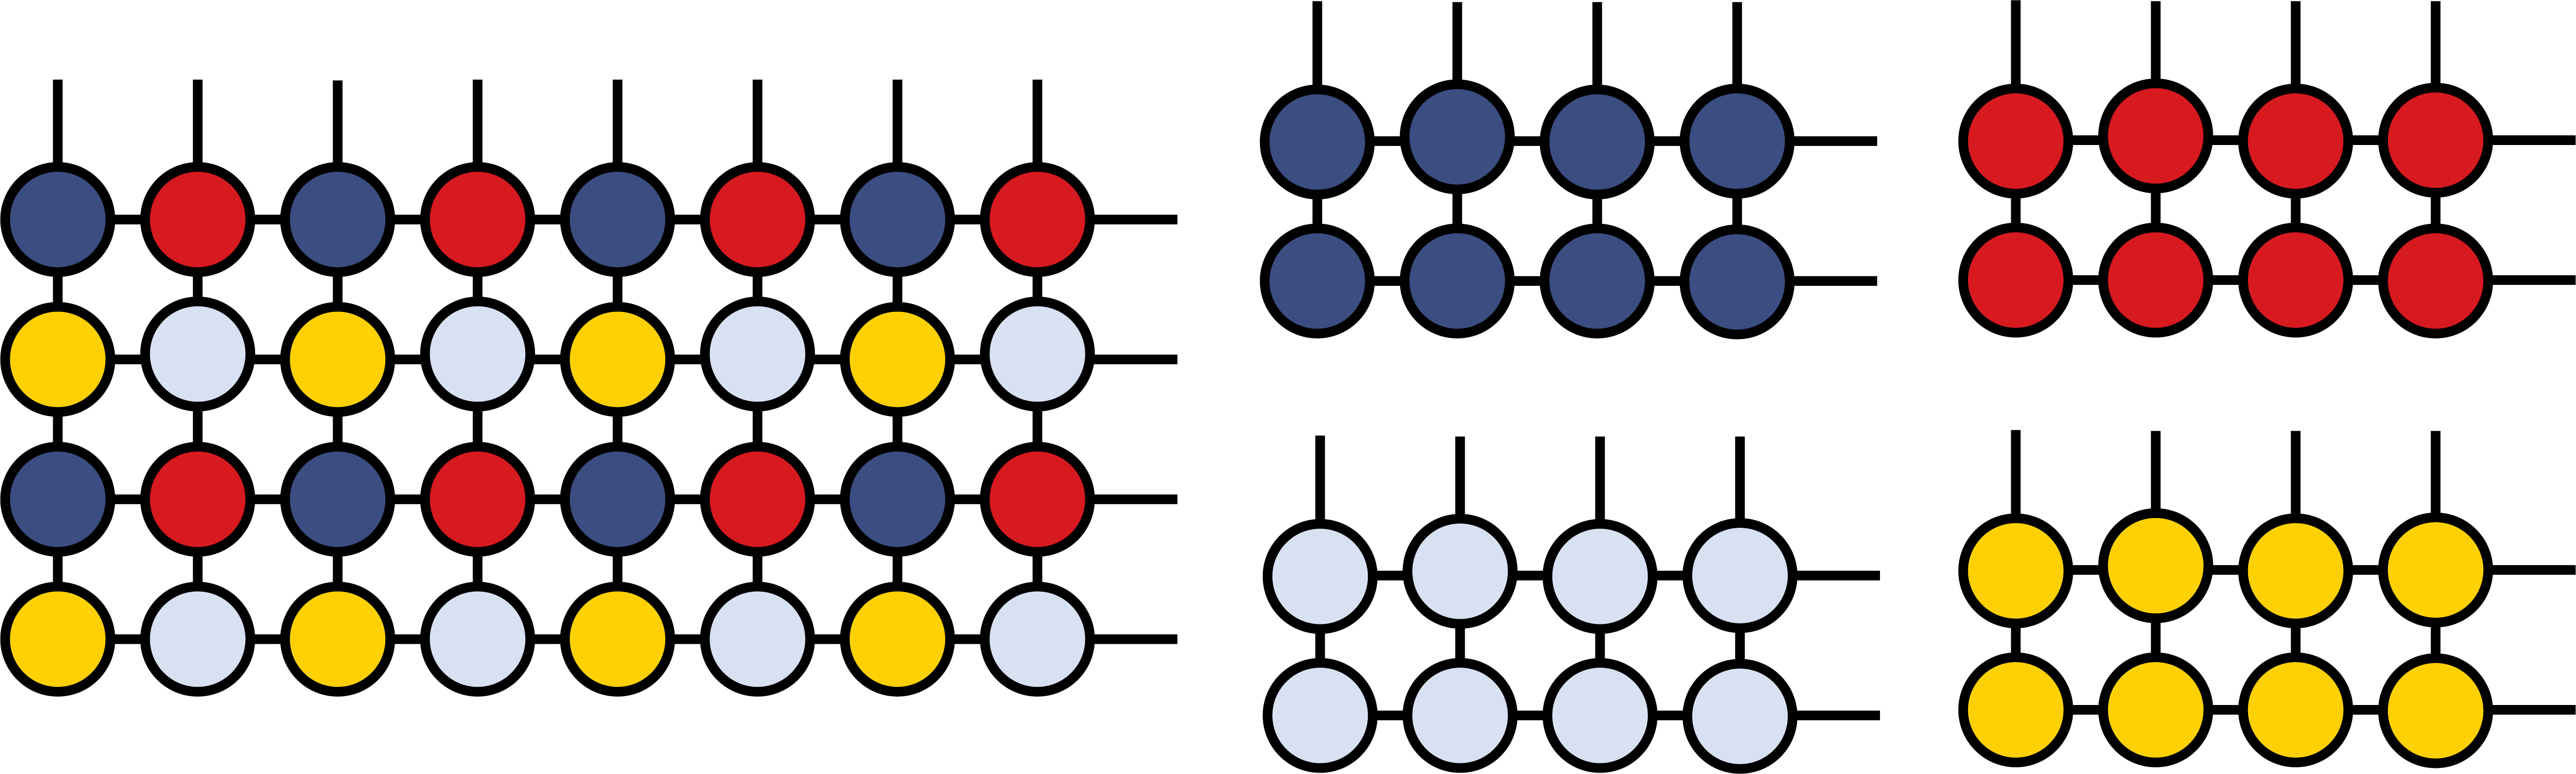
\includegraphics[width=0.9\textwidth]{images/TopOpt/GS_Grid}\\
\end{subfigure}
\begin{subfigure}[b]{.5\textwidth}
\raisebox{0.8cm}{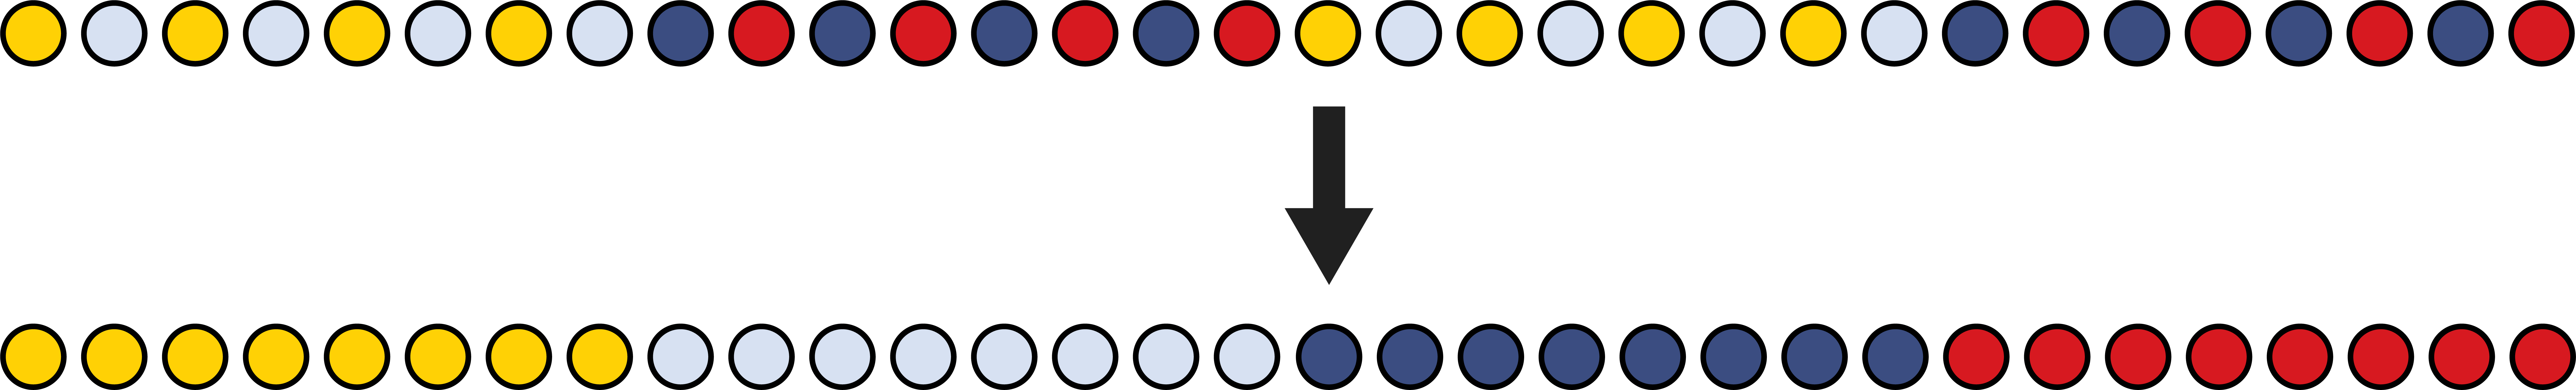
\includegraphics[width=0.9\textwidth]{images/TopOpt/GS_Grid_Linear}}
\end{subfigure}
\caption{Left: a SPGrid block of 4x8 in which the nodes are ordered lexicographically, Right: the transposed colored storage enables efficient vectorization for Gauss-Seidel iteration.
Bottom: Transposition operation of a SPGrid block illustrated in a linear memory layout.}
\label{fig:gs_blocks}
\end{figure}

\paragraph{A mixed-precision MGPCG solver} The linear systems arising from the equations of elasticity in our large-scale topology optimization tasks impose a unique set of
challenges to the numerical algorithms used. Due to both the sheer size of the computational domains we seek to accommodate, and the large contrast of material stiffness values used in
different regions of the simulated domain, we often encounter situations where an MGPCG solver using single-precision (32-bit) floating-point arithmetic cannot sustain satisfactory
convergence, or even instances where the solver will plainly diverge. There are also scenarios where single precision will have catastrophic consequences on our solver, when
Galerkin-coarsened matrices will be reported as effectively ``singular'' by direct solvers (i.e. MKL PARDISO) if constructed to single precision. We note that the frequency of incidence
of such issues was dramatically increased, in our experience, when dealing with domains in excess of $10^8$ voxels, while lower-resolution problems would be significantly more resilient.

An MGPCG solver implemented natively in double precision was fully effective for all the examples in our paper. However, using double precision would double our memory footprint, which
was a significant concession given our pursuit of exceptionally high-resolution domains. We thus designed a variant of such solver that used a carefully crafted mix of single- and
double-precision arithmetic, which we have found to produce results of effectively identical accuracy as a native double-precision solver. Consider the main loop of a 
preconditioned conjugate gradients algorithm, as captured in the following pseudocode:
\begin{figure}[h]
\center
\fbox{
\begin{minipage}{5.5cm}
\vspace*{-.2in}
\begin{align}
\mbox{\textbf{for}}\ \ k=1:N\hspace*{-.3in}\nonumber\\
\color{blue}{\mathbf{q}_k} &\leftarrow \color{purple}{\mathbf{A}}\color{blue}{\mathbf{p}_k}\label{eqn:op-multiply} \\
\color{blue}{\alpha_k} &\leftarrow \color{blue}{\mathbf{r}_k}^{\color{black}{T}} \color{blue}{\mathbf{z}_k} \color{black} / \color{blue}{\mathbf{p}_k}^{\color{black}{T}} \color{blue}{\mathbf{q}_k}\nonumber \\
\color{purple}{\mathbf{x}_{k+1}} &\leftarrow \color{purple}{\mathbf{x}_{k}} \color{black}{+} \color{blue}{\alpha_k} \color{blue}{\mathbf{p}_k}\label{eqn:x-acc}\\
\color{blue}{\mathbf{r}_{k+1}} &\leftarrow \color{blue}{\mathbf{r}_{k}} \color{black}{-} \color{blue}{\alpha_k} \color{blue}{\mathbf{q}_k}\nonumber\\
\color{blue}{\mathbf{z}_k} &\leftarrow \color{purple}{\mathbf{M}^{-1}}\color{blue}{\mathbf{r}_k} \label{eqn:preconditioner}\\
\color{blue}{\beta_k} &\leftarrow \color{blue}{\mathbf{z}_{k+1}}^{\color{black}{T}}\color{blue}{\mathbf{r}_{k+1}} \color{black} / \color{blue}{\mathbf{z}_{k}}^{\color{black}{T}}\color{blue}{\mathbf{r}_{k}} \nonumber\\
\color{blue}{\mathbf{p}_{k+1}} &\leftarrow \color{blue}{\mathbf{z}_{k+1}} \color{black}{+} \color{blue}{\beta_k} \color{blue}{\mathbf{p}_k}\nonumber
\end{align}
\end{minipage}
}
\end{figure}
Our modifications which yield a mixed-precision implementation are summarized as follows:
\begin{itemize}
\item Vectors $\mathbf{r},\mathbf{q},\mathbf{z}$ and $\mathbf{p}$ (colored blue, above) are persistently stored in single-precision floating-point variables. 
\item The solution $\mathbf{x}$ is stored in double precision. The accumulation operation in (\ref{eqn:x-acc}) is also performed in double precision.
\item The operator application in line (\ref{eqn:op-multiply}) is performed in double precision (the single-precision input $\mathbf{p}$ is up-cast to double precision prior to the multiplication). The result of the operator application is then truncated to single precision and stored into $\mathbf{q}$.
\item The multigrid V-cycle used as the preconditioner $\mathbf{M}^{-1}$ in line (\ref{eqn:preconditioner}) is modified as follows: The smoother at the finest level uses double precision
  for the application of the operator, just as in line (\ref{eqn:op-multiply}), although inputs and outputs are stored in single-precision. Every level of the V-Cycle other than the
  finest uses double-precision arithmetic entirely.
\end{itemize}
\begin{figure*}[t!]
\includegraphics[width=1\linewidth]{images/TopOpt/wing}
\caption{An optimized interior supporting structure of part of a wing is generated using our algorithm on a $1696\times 342\times1971$ grid ($402$ M active voxels).}
\label{fig:wing}
\end{figure*}
Using this mixed-precision approach, the memory footprint of our solver is further reduced, providing a significant boost in the maximum resolution we can accommodate for a given amount of physical memory (128 bytes/node suffice to store all variables necessary for the MGPCG solver as well as the minimum compliance optimizer). Our results and validation section provides experimental evidence indicating that this mixed-precision approach yields almost identical accuracy of final
results in all our tests.

\section{Multigrid Solver Validation}\label{sec:topopt_result}

Algorithmically, our implementation of the solver is a standard multi-linearly interpolated Garlerkin-coarsened Multigrid preconditioned conjugate gradient method. At early topology optimization iterations or small domains, such method proves to have fast asymptotic convergence. But in our examples, especially the bird beak Figure \ref{fig:beak} and the wing Figure \ref{fig:wing}, the high variation of material spatial distribution has challenged the convergence of the multigrid solver as shown by Figure \ref{fig:convergence_bird} (left). Thiner features resulted from Higher resolution, can significantly impact the convergence of multigrid as indicated in Figure \ref{fig:convergence_bird} (right).
\begin{figure}[t]
\includegraphics[width=1\linewidth]{images/TopOpt/Convergence_test}	
\caption{(Left) Convergence comparison of the bird beak example of different resolutions at the last topology optimization iteration.  (Right) Convergence comparison of the one-billion-voxel bird beak example at different topology optimization iterations. All residuals reported in this work are $L_{\infty}$ norm across all active cells, normalized relative to the $L_{\infty}$ norm of the load.}
\label{fig:convergence_bird}
\end{figure}

Besides convergence, the high resolution has also pushed the numerical limited of floating point. To validate our mixed precision scheme, we have conducted the following tests, both on analytical structures and the structures naturally emerged from topology optimization: 1. The last iteration of the bird beak example; 2. The last iteration of the wing example; 3-8. Homogeneous and isotropic cantilever beams of different length with one side fixed and the other side loaded with a uniform downward force. 


Table \ref{tab:mix_precision} shows the final residual of five different precision schemes: 1. Full double precision; 2. Only solution vector and computation are in double precision, the mix precision scheme we used in our topology optimization; 3. Only solution vector is in double precision; 4. Only computation is in double precision; 5. All in float precision. The results shows that under all examples our proposed mix precision scheme(column 2) can reduce the residual to an order of magnitude close to the double precision. Due to the fact that at high resolutions, cells that are far from Dirichlet boundaries have large displacements but yet only small strains. This loss of precision leaves it insufficient to use single precision for the solution vector. As shown in (column 4 and 5), using single precision for solution can result in inaccurate computation of strain and final residual. Similarly, using single-precision multiply will not be able to compute search direction to sufficient accuracy, conjugate gradient, in this case, will halt due to a detected singularity (column 3 and 5). 

\newpage
\begin{table*}
\centering
\tiny
\caption{The final residuals of different precision scheme after the same number of iterations. Test cases include bird beak, plane wing, and cantilever beam (CB) with different resolutions. The final residuals are recomputed based on solution vectors. All tests are scaled to initial residual infinity norm of 1. From the left to right, the 5 schemes are: 1. Full double precision; 2. Only solution vector and computation are in double precision; 3. Only solution vector is in double precision; 4. Only computation is in double precision; 5. All in float precision. SINGULAR indicates conjugate gradients have halted due to detected singularity.}
{
\begin{tabularx}{.95\linewidth}{l@{\hskip3.5pt}lXXXXX}
\toprule
	Example			& Double Precision 	& Mix Precision	\newline (double multiply) 	& Mix Precision \newline (single multiply) & Single Precision \newline (double multiply) & Single Precision \newline (single multiply) \\
  	\midrule
	Bird beak	& 	9.192e-5	& 	9.063e-5	& 	1.969e-4 	& 	6.846e+0 	&	7.611e+0 	\\
    Wing		&	8.968e-5	&	1.815e-4	&	SINGULAR	&	1.850e+1	& 	SINGULAR	\\
    CB (32x32x32)	&	7.942e-6	&	7.942e-6	& 5.827e-5	& 2.259e-5	&	5.827e-5	\\
    CB (32x32x64)	&	8.217e-6	&	8.218e-6	& 5.773e-5	& 4.905e-5	&	6.019e-5	\\
    CB (32x32x128)	&	8.207e-6	&	8.208e-6	& 1.041e-3	& 1.018e-4	&	1.041e-3	\\
    CB (32x32x256)	&	9.322e-6	&	9.321e-6	& 6.295e-3	& 1.934e-4	&	6.295e-3	\\
    CB (32x32x512)	&	4.506e-6	&	4.508e-6	& SINGULAR	& 3.990e-4	&	SINGULAR	\\
    CB (32x32x1024)&	5.237e-6	&	5.242e-6	& SINGULAR	& 7.043e-4	&	SINGULAR	\\
    \midrule
\end{tabularx}
}
\label{tab:mix_precision}
\end{table*}


\chapter{Stencil Aware Galerkin Coarsened Multigrid for Linear Elasticity} 
\label{Chapter:BBMG}
In Chapter~\ref{Chapter:Elasticity}, we have examined an efficient implementation of a standard multilinear Galerkin coarsened multigrid preconditioned conjugate gradient algorithm for linear elasticity. In figure~\ref{fig:convergence_bird}, we have observed that with the increasing of resolution (left), and domain complexity(right). The MGPCG convergence is severely impaired. In this chapter, as a continuation to  Chapter~\ref{Chapter:Solver}, we will examine the design of a stencil aware Galerkin coarsened multigrid and its efficacy when solving complex domains in comparison to multilinear interpolated Galerkin coarsened multigrid.
\section{Selection of Coarse Grid Nodes and Prolongation Operator Sparsity}
\label{sec:p_sparsity}
In this chapter, I will present a multigrid method for solving linear elasticity problems discretized with 3D eight-node brick elements on a Cartesian grid. Therefore, the position of node $(i,j,k)$ in undeformed space $\mathbf{X}$, can be written as:
$$
\mathbf{X}(i,j,k) = (i*h,j*h,k*h), (i,j,k) \in G^0
$$
Here, $h$ is the element length. $G^0$ is the finest level discretization.We wish to maintain the regularity across all levels. Therefore, we can write the position of node $(i,j,k)$ in undeformed space $\mathbf{X}$ at level 1 as:
$$
\mathbf{X}(i,j,k) = (i*2h,j*2h,k*2h), (i,j,k) \in G^1
$$
And so on for the coarser levels. Now that we have selected the coarse grid degrees of freedom, a proper prolongation operator is required for building the multigrid hierarchy. Given that the finest level operator $\mathbf{L}^0$ has a regular $27$ point stencil sparsity, we wish that all coarse level operators $\mathbf{L}^c$ shares the same sparsity. Here I will propose a sparsity pattern for the prolongation operator that guarantees such property, though it is not the only one that satisfies, but it is most commonly used, and fits well with the methods for computing the prolongation operator in the next sections.
\begin{enumerate}
\item If a fine node $f$ is coincide with a coarse node $c$ in undeformed space, $P_{fc^*} = 0$, if $c^* \neq c$
\item If a fine node $f$ lies on a coarse element edge in undeformed space. If coarse node $c_1$ and $c_2$ define this edge, $P_{fc^*} = 0$, if $c^* \neq c_1$ and $c^* \neq c_2$, Figure~\ref{fig:neighbor_ring}.
\item If a fine node $f$ lies on a coarse element face in undeformed space. If coarse node $c_1$, $c_2$, $c_3$, and $c_4$ define this face, $P_{fc^*} = 0$, if $c^* \neq c_p$, $\forall c_p \in \{c_1,c_2,c_3,c_4\}$.
\item If a fine node $f$ lies on a coarse element center in undeformed space. If coarse node $c_1$, $c_2$, $c_3$, $c_4$, $c_5$, $c_6$, $c_7$, and $c_8$ define this coarse element, $P_{fc^*} = 0$, if $c^* \neq c_p$, $\forall c_p \in \{c_1,c_2,c_3,c_4,c_5,c_6,c_7,c_8\}$.
\end{enumerate}
 Note that these rules create same coarse nodes and prolongation operators that is of exact same sparsity as a standard multilinearly interpolated prolongation operators in Chapter~\ref{Chapter:Elasticity}.
\section{Building Prolongation Operator Using Local Problems}
\subsection{Define Local Matrix}
In section~\ref{sec:Convergence_Metric}, we stated that the quality of the prolongation operator can be measured by two metrics:
 \begin{equation}
M_1(\mathbf{Q},\mathbf{e}) := \frac{<(\mathbf{I}-\mathbf{Q})\mathbf{e}, (\mathbf{I}-\mathbf{Q})\mathbf{e}>}{<\mathbf{L}\mathbf{e},\mathbf{e}>}
\end{equation}
\begin{equation}
M_2(\mathbf{Q},\mathbf{e}) := \frac{<\mathbf{L}(\mathbf{I}-\mathbf{Q})\mathbf{e}, (\mathbf{I}-\mathbf{Q})\mathbf{e}>}{<\mathbf{L}\mathbf{e},\mathbf{e}>}
\end{equation}
Here we take $\mathbf{Q}$ as:
$$
  \mathbf{Q} = \left[ \begin{array}{cc}
    \mathbf{0} & \mathbf{P}_{cf} \\
    \mathbf{0} & \mathbf{I}_c
  \end{array}\right]\\
$$
But both measurement requires the global operator $\mathbf{L}$. In work \cite{brezina2001algebraic}, an alternative local operator $\mathbf{L}_i$ is proposed. $\mathbf{L}_i$ is the sum of the element stiffness matrix adjacent to a given fine node $i$.
\begin{equation}
\mathbf{L}_i = \sum_{\alpha\in \mathcal{T}_i} L_\alpha
\label{equ:local_matrix}
\end{equation}
$L_\alpha$ is the elemental stiffness matrix of element $\alpha$, $\mathcal{T}$ is one ring neighborhood, illustrated in Figure~\ref{fig:neighbor_ring}.
\begin{figure}[t]
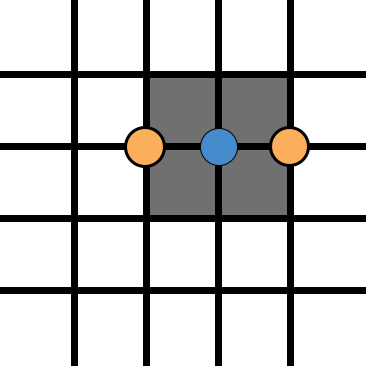
\includegraphics[width=4cm]{BBMG/neighbor.png}
\centering
\caption{A neighborhood of a given fine node, shaded in blue, in Cartesian discretization. The neighboring cells of the given node is shaded in gray. In this case, we are interpolating the fine node values from the given coarse nodes, shaded in yellow.}
\label{fig:neighbor_ring}
\end{figure}
The localized measurement $M_{i,1}$ and $M_{i,2}$ can then be defined as:
 \begin{equation}
M_{i,1}(\mathbf{Q},\mathbf{e}) := \frac{<\epsilon_i\epsilon^T_i(\mathbf{I}-\mathbf{Q})\mathbf{e}, \epsilon_i\epsilon^T_i(\mathbf{I}-\mathbf{Q})\mathbf{e}>}{<\mathbf{L}_i\mathbf{e},\mathbf{e}>}
\end{equation}
\begin{equation}
M_{i,2}(\mathbf{Q},\mathbf{e}) := \frac{<\mathbf{L}_i\epsilon_i\epsilon^T_i(\mathbf{I}-\mathbf{Q})\mathbf{e}, \epsilon_i\epsilon^T_i(\mathbf{I}-\mathbf{Q})\mathbf{e}>}{<\mathbf{L}_i\mathbf{e},\mathbf{e}>}
\end{equation}
Here $\epsilon_i$ is a vector, that its entries satisfies:
$$
\epsilon_i(j) = \delta_{ij} 
$$
$\delta$ is the Kronecker delta. If we denote the set of projection operators $\mathbf{Q}$ that satisfies those sparsity conditions stated in section~\ref{sec:p_sparsity} as $\mathcal{Z}_i$. The $i$th row if $\mathbf{Q}$ is then:
$$
\mathbf{q}^T_i = \epsilon^T_i\mathbf{Q}
$$
 Then finding the prolongation operator for a given fine node $i$ can be expressed as the following min-max problem:
 \begin{align}
 K_{i,p} = \min_{q_i \in \mathcal{Z}_i} \max_{\mathbf{e}\perp \text{Null}(\mathbf{L}_i)} M_{i,p}(\mathbf{q}_i,\mathbf{e})\nonumber\\
 \text{subject to } (\epsilon_i - \mathbf{q}_i) ^ T \mathbf{e} = 0\text{, }\forall \mathbf{e} \in \text{Null}(\mathbf{L}_i) \label{equ:local_metric}
 \end{align}
 The condition in equation~\ref{equ:local_metric}, states that the prolongation operator must correctly interpolate local null space. For Poisson problems, the nullity of the local matrix is only 1. But for elasticity problems the nullity of the local matrix is drastically raised to 6 in 3D. Three degrees of displacements and three degrees rotations. 
 \subsection{Computation of the Prolongation Operator}
 For the local problem defined above with fine node $i$, we denote the set of nodes included in this local problem as $\mathcal{N}_i$. We write $c$ as the coarse nodes that fine node $i$ is interpolated from. $f$ as the fine nodes from $\mathcal{N}_i$. $n_c$ is the size of the set $c$, and $n_f$ is the size of the set $f$. Then we can write the local matrix $L_i$ as:
 $$
\mathbf{L}_i = \begin{bmatrix} 
 \mathbf{L}^{(1)}_{ff} & \mathbf{L}^{(1)}_{fc} \\
 \mathbf{L}^{(1)}_{cf} & \mathbf{L}^{(1)}_{cc}
 \end{bmatrix}
 $$
 for metric $M_{i,1}$, and:
  $$
 \mathbf{L}^2_i = \begin{bmatrix} 
 \mathbf{L}^{(2)}_{ff} & \mathbf{L}^{(2)}_{fc} \\
 \mathbf{L}^{(2)}_{cf} & \mathbf{L}^{(2)}_{cc}
 \end{bmatrix}
 $$
 for metric $M_{i,2}$. If we place node $i$ as the first of all the nodes $f$. we can replace $\epsilon_i$ with $\epsilon_1$ in the two local metrics. 
 
\begin{lem}\label{lemma:q_existance}There exits $\mathbf{q}_i \in \mathcal{Z}_i$, such that $\epsilon_1 - \mathbf{q}_i \in \text{Range}(\mathbf{L}^p_i)$ if and only if
$$
\hat{\epsilon}_1 \in \text{Range}(\mathbf{L}^{(p)}_{ff})
$$
$\hat{\epsilon}_1$ is the first canonical basis vector of length $n_f$. $p = 1\text{ or }2$.
\end{lem}
Lemma~\ref{lemma:q_existance} simply state that there exists an interpolation that interpolates null space correctly, if the fine node $i$ does not have a zero diagonal.
\begin{theorem}
\label{theo:p_solution}
If $\hat{\epsilon}_1 \in \text{Range}(\mathbf{L}^{(p)}_{ff})$, than $K_{i,p} = \infty$. If $\hat{\epsilon}_1 = \mathbf{L}^{(p)}_{ff} \hat{\delta}_1$, then the unique solution of equation~\ref{equ:local_metric} is given by
\begin{equation}
\mathbf{q}_i^* = \left(\begin{array}{c}0 \\ -\mathbf{L}^{(p)}_{cf}\hat{\delta}_1\end{array}\right)  \in \mathcal{Z}
\end{equation}
and $K_{i,p} = <\hat{\epsilon}_1,\hat{\delta}_1>$, for $p = 1\text{ or }2$.
\end{theorem} 
First part of Theorem~\ref{theo:p_solution} states that if there is no solution exists, multigrid can not converge for the error mode containing node $i$. From Lemma~\ref{lemma:q_existance}, there is no solution if node $i$ has zero diagonal. Therefore any error modes that has a non-zero error for node $i$, is in the null space of the original matrix, then there is no solution to the original matrix.

Second part of Theorem~\ref{theo:p_solution}, states how we can compute the prolongation operator:
\begin{align*}
\hat{\epsilon}_1 &= \mathbf{L}^{(p)}_{ff}\hat{\delta}_1\\
\hat{\delta}_1 &= (\mathbf{L}^{(p)}_{ff})^{(-1)}\hat{\epsilon}_1\\
\mathbf{q}_i^* &= (\mathbf{e}^T_i\mathbf{Q})^T\\
&= \mathbf{Q}^T\epsilon_i \\
&= \left(\begin{array}{c} 0 \\ \mathbf{P}^T_{fc}\epsilon_i\end{array}\right) \\
&= \left(\begin{array}{c}0 \\ -\mathbf{L}^{(p)}_{cf}\hat{\delta}_1\end{array}\right) \\
\mathbf{P}^T_{fc}\epsilon_i &=  -\mathbf{L}^{(p)}_{cf}\hat{\delta}_1 \\
&= -\mathbf{L}^{(p)}_{cf}(\mathbf{L}^{(p)}_{ff})^{-1}\hat{\epsilon}_1
\end{align*}
$\mathbf{P}^T_{fc}\epsilon_i$ is a row of the prolongation operator. A practical way for computing it when using metric $M_{i,1}$, is to set the coarse nodes in the local problem as Dirichlet. By setting each degrees of freedom $j$ with value of $1$, i.e. a Kronecker delta. Solving the local problem, the value(s) of the DOF of fine node $i$ is then the entry $\epsilon^T_i\mathbf{P}_{fc}\epsilon_j$.
Here each row of the prolongation operator is the harmonic extension of a canonical basis vector.
If reader are interested in the proof of Lemma~\ref{lemma:q_existance} and Theorem~\ref{theo:p_solution}, I refer reader to \cite{brezina2001algebraic}. Here, I will only use the result and viewing their implications. Furthermore, it is worth noting that in work \cite{henson2001element}, an alternative formulation of equation~\ref{equ:local_metric} in the perspective of energy minimization was proposed, upon which work \cite{dohrmann2007interpolation} was based. As it is unimportant for the derivation of our method, I will omit that formulation here.
\section{Multigrid Method with Augmented Variables}
Condition of equation~\ref{equ:local_metric}, states that prolongation operator must correctly interpolate error vectors $\mathbf{e}$ that are in the Null space of the local matrix $\mathbf{A}_i$. Here I will give without prove that standard multi-linear interpolation satisfies this condition for both elasticity and Poisson problems, as it is used for homogeneous problems and proven to be effective. In section~\ref{sec:p_sparsity}, a sparsity condition for the prolongation operator was imposed to guarantee the sparsity of the coarse level operators. Considering Figure~\ref{fig:neighbor_ring}, that the fine node is interpolated from the edge adjacent two coarse nodes. For 3D elasticity, the two coarse nodes provides 6 equations in solving the local prolongation operator. Note that the Nullity of $\mathbf{A}_i$ is also 6. Which means there is only one prolongation operator satisfies the condition of equation~\ref{equ:local_metric}, and we know that the standard multi-linear interpolation satisfies this condition. Therefore:
\begin{lem}\label{lemma:linear_best} 
 Multi-linear interpolation is the \textbf{only} interpolation that can capture error vectors in the null space of local matrix $\mathbf{A}_i$ for fine nodes that are interpolated from only two coarse nodes in 3D elasticity problems.
\end{lem}
Given that the largest $M_{i,p}$ is the upper bound for the multigrid convergence rate, which means it is very difficult to improve the convergence over multi-linear interpolated multigrid while maintaining our sparsity constraints for the prolongation operator. In work \cite{dohrmann2007interpolation}, similar observations were made. By introducing additional degrees of freedom in the coarse grids, better solutions to equation~\ref{equ:local_metric} can be achieved. 
\subsection{Introducing Linearized Rotational Degrees of Freedom}
Similar to \cite{dohrmann2007interpolation}, we introduced linearized rotational degrees of freedom to the coarse grid to improve the quality of the prolongation operator. But different from it, given that our top level operator is matrix free as stated in chapter~\ref{Chapter:elasticity}, we can easily compute the element matrix on the top level and therefore avoiding the local null space analysis suggested in \cite{dohrmann2007interpolation}. First, I will introduce the additional linearized rotational DOF and their physical interpolation, then an algorithm will be provided for computing the solution given by theorem~\ref{theo:p_solution} with the extended DOF.
\begin{figure}[t]
\includegraphics[width=5cm]{BBMG/rotation.png}
\centering
\caption{A 2D example of a rotational degree of freedom $\theta$ and its physical interpolation in the case of interpolation fine node, marked blue, that is aligned with a coarse cell edge from two adjacent coarse nodes, marked yellow. Letters are associated names for the nodes. The solid lines indicates the deformed cells. The doted lines illustrated the undeformed cells.}
\label{fig:rotation_2D}
\end{figure}
Figure~\ref{fig:rotation_2D} illustrates the deformation created by the rotation DOF $\theta_L$ of node \textit{L} in 2D. The rotational degrees of freedom associated with node \textit{L}, namely $\theta_L$, is viewed influence the horizontal, and only the horizontal displacement of nodes \textit{LT} and \textit{LB}. If we write the the coarse DOF of node \textit{L}, displacements and rotation, denoted $\mathbf{u}^c_L$ for the local problem as:
$$
\mathbf{u}^c_L = \left(\begin{array}{c}u^c_L(x) \\ u^c_L(y) \\ u^c_L(\theta) \end{array}\right)
$$
The superscript $^c$ here indicates the DOF live on the coarse grid. Accordingly, the fine DOF of nodes \textit{LT}, \textit{L}, and \textit{LB}, then can be computed accordingly:
\begin{align*}
 \mathbf{u}^f_{LT} &= \left(\begin{array}{c} u^c_L(x) - u^c_L(\theta)h \\ * \end{array}\right) \\
 \mathbf{u}^f_{L} &= \left(\begin{array}{c} u^c_L(x) \\ u^c_L(y) \end{array}\right) \\
 \mathbf{u}^f_{LB} &= \left(\begin{array}{c} u^c_L(x) + u^c_L(\theta)h \\ * \end{array}\right) 
\end{align*}
$h$ is the cell width. The symbol $*$ indicates that this DOF is not fixed for the local problem for interpolating the fine grid node values $\mathbf{u}^f_{C}$. Similarly we can write the right side nodal values as:
\begin{align*}
 \mathbf{u}^f_{RT} &= \left(\begin{array}{c} u^c_R(x) - u^c_R(\theta)h \\ * \end{array}\right) \\
 \mathbf{u}^f_{R} &= \left(\begin{array}{c} u^c_R(x) \\ u^c_R(y) \end{array}\right) \\
 \mathbf{u}^f_{RB} &= \left(\begin{array}{c} u^c_R(x) + u^c_R(\theta)h \\ * \end{array}\right) 
\end{align*}
So if we rearrange the local matrix in equation~\ref{equ:local_matrix}, so that nodal values $\mathbf{u}^f_{C}$ first, then the other undetermined(or free) nodal values, and last, the eight determined nodal values we write as vector $\mathbf{u}^f_{D}$: 
$$
\mathbf{u}^f_{D} = \left(\mathbf{u}^f_{LT}(x), \mathbf{u}^f_{LT}(x), \mathbf{u}^f_{LT}(y), \mathbf{u}^f_{LB}(y),\mathbf{u}^f_{RT}(x), \mathbf{u}^f_{RT}(x), \mathbf{u}^f_{RT}(y), \mathbf{u}^f_{RB}(y)\right)
$$
We denote the rearranged local matrix as: 
 \begin{equation}
 \label{equ:matrix_split}
\mathbf{L}_i = \begin{bmatrix} 
\mathbf{L}_{ff} & \mathbf{L}_{fd} \\
\mathbf{L}_{df} & \mathbf{L}_{dd}
\end{bmatrix}
\end{equation}
 Here $\mathbf{L}_{dd}$ is a $8\times8$ matrix, $\mathbf{L}_{ff}$ is of dimension $10\times10$. Based on theorem~\ref{theo:p_solution}, the free fine nodal DOF vector $\mathbf{u}^f$ of size $10$ can than be computed as:
 \begin{equation}
 \mathbf{u}^f = -(\mathbf{L}_{ff})^{-1}\mathbf{L}_{fc}\mathbf{u}^f_D
 \end{equation} 
 Given that each component in vector $\mathbf{u}^f_{D}$ can be computed from $\mathbf{u}^c_L$ and $\mathbf{u}^c_R$ using a linear transformation. We can construct a transformation matrix $T$, s.t.:
   \begin{equation}
   \mathbf{u}^f_D = \mathbf{T} \mathbf{u}^c
   \end{equation}
   The local prolongation operator is therefore:
 \begin{equation}
 \mathbf{P}_i = -(\mathbf{L}_{ff})^{-1}\mathbf{L}_{fd}\mathbf{T}
 \label{equ:edge_P_2D}
 \end{equation}
The first two rows of  $\mathbf{P}_i$ is the prolongation operator for the fine node $i$. By using $\mathbf{L}_i$ instead of $\mathbf{L}^2_i$, our local convergence metric is therefore $M_{1,q}$. 
\subsection{Interpolation of Cell Centered Nodes in 2D}
Now that, we have interpolated the fine nodes that are aligned with the coarse cell edges. The next step is interpolating the fine nodes that are located in the center of the coarse cells, Figure~\ref{fig:embedded_interpolation}
\begin{figure}[t]
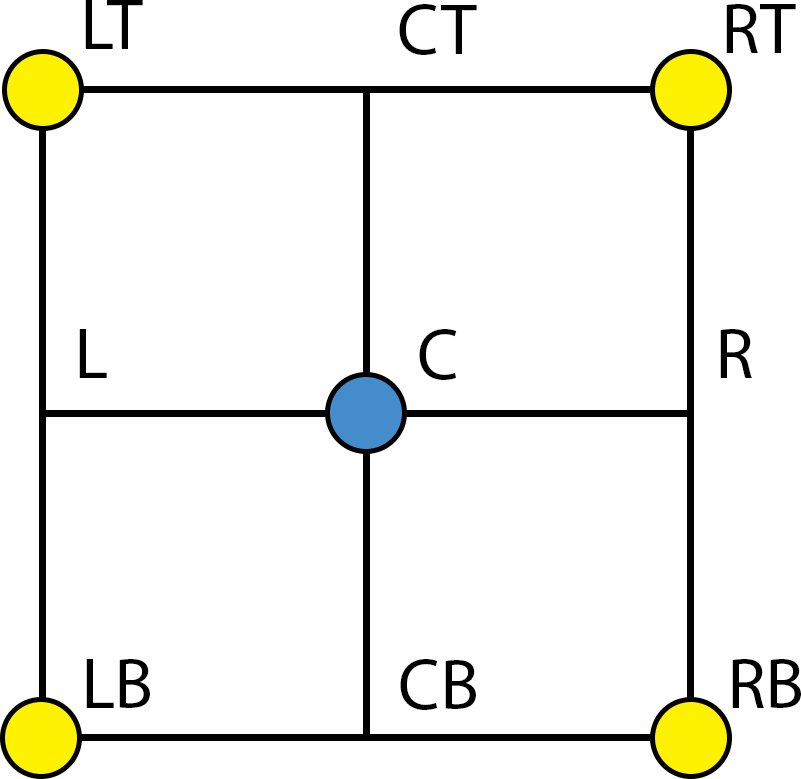
\includegraphics[width=5cm]{BBMG/Embeded_Interpolation}
\centering
\caption{Interpolation of a fine node, blue, that is in the center of a coarse cell. The coarse nodes are shaded in yellow. Each node is given a name.}
\label{fig:embedded_interpolation}
\end{figure}
Notice here that node \textit{CT} can be interpolated from node \textit{LT} and \textit{RT}. Similarly to node \textit{L},  \textit{R}, and \textit{CB}. As a matter of facts, that all the 8 neighbors of node \textit{C} can be interpolated. So, we can prolongate the node \textit{C} that has zero residual at the fine level. If $i$ is the index of node \textit{C}, and $\mathcal{N}_i$ is the set of nodes that are adjacent to node $i$, i.e.:
$$
\mathcal{N}_i = \{\textit{LB},\textit{CB},\textit{RB},\textit{L},\textit{R},\textit{LT},\textit{CT},\textit{RT}\}
$$
We can solve value of node $i$, denoted as $\mathbf{u}^f_i$ as:
\begin{equation}
\mathbf{L}_{ii}\mathbf{u}^f_i + \sum_{j \in \mathcal{N}_i}\mathbf{L}_{ij}\mathbf{P}_j\mathbf{u}^c = 0 
\end{equation}
Here $\mathbf{P}_j$ is the $j$th rows of the prolongation operator that computes the nodal values of $j$. In 2D, it is $2$ rows, and in 3D, it is three rows. So $\mathbf{P}_j\mathbf{u}^c$ computes the nodal value vector $\mathbf{u}^f_j$. $\mathbf{L}_{ij}$ is the stencil coefficient coupling node $j$ and $i$. It is a $2 \times 2$ matrix in 2D and $3 \times 3$ matrix in 3D. Therefore we can write the solution to $\mathbf{u}^f_i$ as:
\begin{equation}
\mathbf{u}^f_i = -\sum_{j \in \mathcal{N}_i}(\mathbf{L}_{ii})^{-1}\mathbf{L}_{ij}\mathbf{P}_j\mathbf{u}^c
\end{equation}
Therefore the prolongation operator for node $i$, $\mathbf{P}_i$ is then:
\begin{equation}
\mathbf{P}_i = -\sum_{j \in \mathcal{N}_i}(\mathbf{L}_{ii})^{-1}\mathbf{L}_{ij}\mathbf{P}_j
\label{equ:p_cell_center}
\end{equation}
\subsection{Interpolation of Fine Nodes that Coincide with a Coarse node in 2D}
This as the simplest case, same as a standard multi-linear interpolation, the fine node displacement are injected from the corresponding coarse node, while the rotational DOF are ignored.
\section{Rotational Degrees of Freedom in 3D}
Fine nodes in 3D can be categorized into 4 types as stated in section~\ref{sec:p_sparsity}:
\begin{enumerate}
\item coincide with a coarse node
\item lies on a coarse cell edge center
\item lies on a coarse cell face center
\item lies on a coarse cell cell center
\end{enumerate}
For case 1 and case 4, the expressions for computing prolongation operator are identical for 2D and 3D. I will focus case 2 and 3, as they are similar to 2D and yet require special treatment. 
\subsection{Interpolating Fine Nodes that Lies on a Coarse Cell Edge Center}
The prolongation operator can be computed with the same formula as equation~\ref{equ:edge_P_2D} as in the 2D case, but the rearrangement of the local matrix is different. Consider a one ring neighborhood of a fine node $i$, $\mathcal{N}_i$ that contains 26 nodes. Without loss of generosity, we assume node $i$ lies on a coarse node edge aligned with the x axis. Therefore if the node $i$ has geometric index $(x_i, y_i, z_i)$ in the Cartesian grid. We are interpolating its value from node $c_1$ with geometric $(x_i - 1, y_i, z_i)$ and node $c_2$ with geometric $(x_i + 1, y_i, z_i)$. If we denote the DOF of the coarse nodes are:
$$
\mathbf{u}^c = \left(\begin{array}{c}u_x\\u_y\\u_z\\r_x\\r_y\\r_z\end{array}\right)
$$
$\mathbf{u}^c_1$ is the vector of nodal values for node $c_1$ and $\mathbf{u}^c_2$ is the vector of nodal values for node $c_2$. The fine node DOF at geometric index $(x_i - 1, y_i, z_i)$ and $(x_i + 1, y_i, z_i)$ is then computed my injection:
 \begin{equation}
 \mathbf{u}^f(x_i - 1, y_i, z_i) = \begin{bmatrix} 
 1 & 0 & 0 & 0 & 0 & 0\\
 0 & 1 & 0 & 0 & 0 & 0\\
 0 & 0 & 1 & 0 & 0 & 0 \end{bmatrix} \mathbf{u}^c_1
 \end{equation}
 Similarly $\mathbf{u}^f(x_i + 1, y_i, z_i)$ can be computed. Now regarding the rotational DOF of a given coarse node, they influence only the fine nodes in $\mathcal{N}_i$ that are connected to the coarse node through an edge and that is not the center fine node $i$. For instance, rotational DOF of node located at coarse node $c_1$ with geometric index $(x_i + 1, y_i, z_i)$, influence the following $4$ fine nodes in $\mathcal{N}_i$.
 \begin{equation}
 \mathcal{R}_1 = \{(x_i - 1, y_i+1, z_i),(x_i - 1, y_i-1, z_i),(x_i - 1, y_i, z_i+1), (x_i - 1, y_i, z_i-1)\}
 \end{equation}
$\mathcal{R}_1$ is the set of nodes influence by rotational DOF of node $c_1$. Similarly we can define $\mathcal{R}_2$. Given the symmetry, without loss of generality, pick node $(x_i - 1, y_i - 1, z_i)$ as an example we can set its nodal value in the local problem as. The vector between the node $(x_i - 1, y_i, z_i)$ and $(x_i - 1, y_i - 1, z_i)$ is $(0,-h,0)$. Again $h$ here is the cell size. If the rotational DOF are $(r_x,r_y,r_z)$. Then we can write the linearized rotational matrix as:
\begin{equation}
\mathbf{R}^c_1 = \begin{bmatrix} 
0 & -r_z & r_y\\
r_z & 0 & -r_x \\
-r_y & r_x & r_z
\end{bmatrix}
\end{equation}
Then displacement of node $(x_i - 1, y_i - 1, z_i)$ caused by the rotation around the coarse node is then:
\begin{equation}
\mathbf{R}^c_1  \left[\begin{array}{c} 0\\-h\\0\end{array}\right] = \left[\begin{array}{c} hr_z\\0\\-hr_x\end{array}\right]
\end{equation}
Here the $2$nd dimension of the displacement is not influence by the rotation of the coarse node. Therefore we set it as an free variable. Now we can write the displacement of node $(x_i - 1, y_i - 1, z_i)$ on the fine grid as:
 \begin{equation}
 \mathbf{u}^f(x_i - 1, y_i, z_i) = \begin{bmatrix} 
 1 & 0 & 0 & 0 & h & 0\\
 * & * & * & * & * & *\\
 0 & 0 & 1 & 0 & -h & 0 \end{bmatrix} \mathbf{u}^c_1
 \end{equation}
 $*$ here means that DOF is set to be a free variable. Now that we have prescribed a selection of fine node DOF in the local problem, we can rearrange the local matrix $\mathbf{L}_i$ similar to equation~\ref{equ:matrix_split}, and compute the prolongation operator similar to equation~\ref{equ:edge_P_2D}.
% \include{motivation/motivation}
% \include{related/related}

%% etc, etc.

%% Do you have appendices?  If so, add them here, just like chapters.
% \begin{appendices}
% \include{backmatter/appendix1}
% \end{appendices}

%% Are you a big nerd with a colophon?  Add it here.
\begin{colophon}
\svnidlong{$LastChangedBy$}{$LastChangedRevision$}{$LastChangedDate$}{$HeadURL: http://freevariable.com/dissertation/trunk/frontmatter.tex $}
\vcinfo{}

This template uses Gyre Pagella by default.  (I used Arno Pro in my dissertation.)

Feel free to give me a shout-out in your colophon or acks if this template is useful for you.  Good luck!

\end{colophon}

%% McBride is a very nice style (some version is included in this distribution)
\bibliographystyle{mcbride}
\bibliography{dissertation}

%% Want an index?  Neither did I.
%\printindex

\end{document}
